%!TEX TS-program = xelatex 
%!TEX encoding = UTF-8 Unicode

\documentclass[School=Princeton]{Dissertate}

\RequirePackage{settings}

% \newglossaryentry{compiler}{
%     name={compiler},
%     description={A program that translates a programming language into another}
% }

% \newglossaryentry{primitive type}{
%     name={primitive type},
%     description={A type that cannot be inspected further}
% }

\newglossaryentry{metaprogramming}{
    name={metaprogramming},
    description={Writing programs that inspect existing programs or generate new programs}
}

\newglossaryentry{shallow embedding}{
    name={shallow embedding},
    description={A description of an object language that uses the semantics of the host language to implement corresponding features}
}

\newglossaryentry{deep embedding}{
    name={deep embedding},
    description={A description of an object language where the syntax tree of the object language is data in the host language}
}

\newglossaryentry{FFI}{
    name={foreign function interface (FFI)},
    description={A multilanguage programming style in which one language imitates the calling conventions of the other languages so that the two languages can call each other. Consists of \gls{foreign function}s and \gls{foreign type}s}
}
\newcommand{\ffi}{\glslink{FFI}{foreign function interface}}
\newcommand{\FFI}{\glslink{FFI}{FFI}}

\newglossaryentry{boxed}{
    name={boxed},
    description={A value that is represented in memory with indirection, such as a pointer into a separate data structure that holds information}
}

\newglossaryentry{unboxed}{
    name={unboxed},
    description={A value that is represented without a memory indirection, as a nonpointer}
}

\newglossaryentry{boxity}{
    name={boxity},
    description={Whether a value is \emph{\gls{boxed}} or \emph{\gls{unboxed}}}
}

\newglossaryentry{inductive type}{
    name={inductive type},
    description={A generalized version of algebraic data types, used for defining custom data types in Coq}
}

\newcommand{\constructor}{\glslink{data constructor}{constructor}}
\newcommand{\Constructor}{\glslink{data constructor}{Constructor}}
\newglossaryentry{data constructor}{
    name={data constructor},
    description={The only way of creating a value of an inductive type. Also simply referred to as ``constructor"}
}

\newglossaryentry{type constructor}{
    name={type constructor},
    description={The name of a type, with no arguments applied, such as \vec{} for the vector type}
}


\newcommand{\parametrized}{\glslink{parameter}{parametrized}}
\newglossaryentry{parameter}{
    name={parameter},
    description={An argument to the inductive type constructor that cannot vary between data constructors of that type}
}

\newcommand{\indices}{\glslink{index}{indices}}
\newglossaryentry{index}{
    name={index},
    description={An argument to the inductive type constructor that can vary between data constructors of that type}
}

\newcommand{\header}{\glslink{header-memory}{header}}
\newglossaryentry{header-memory}{
    name={header (memory)},
    description={An extra field where metadata about whatever comes afterwards can live}
}

\newcommand{\glue}{\glslink{glue code}{glue}}
\newglossaryentry{glue code}{
    name={glue code},
    description={Functions that help programmers inspect, construct, or call one language's values from another language. For CertiCoq's generated glue code, see \autoref{glue}}
}

\newcommand{\tinfo}{\glslink{thread info}{\bn{tinfo}}}
\newglossaryentry{thread info}{
    name={thread info},
    description={A C \kw{struct} that holds the necessary information for the CertiCoq runtime to work, such as the call stack, the location of the \gls{CertiCoq heap}, and the location of the next allocatable spot in that heap. Often shortened to \tinfo{} when used in code}
}

\newglossaryentry{CertiCoq heap}{
    name={CertiCoq heap},
    description={The region in memory the CertiCoq runtime primarily operates on, and is garbage collected by the CertiCoq runtime}
}
\newglossaryentry{C heap}{
    name={C heap},
    description={The region in memory outside of the \gls{CertiCoq heap}. Memory management of this region is the user's responsibility}
}

\newglossaryentry{tag}{
    name={tag},
    description={The index of a constructor in the inductive type definition. Not the same thing as an \gls{ordinal}}
}

\newglossaryentry{ordinal}{
    name={ordinal},
    description={The index of a constructor within the constructors of that inductive type with the same \gls{boxity}. Not the same thing as a \gls{tag}}
}

\newglossaryentry{closure}{
    name={closure},
    description={The value form of a function in a functional programming language. It consists of a function and an environment, where the environment contains values for the free variables in the function body}
}

\newglossaryentry{locally nameless}{
    name={locally nameless},
    description={A representation for variables where free variables are represented as names, while bound variables are represented as de Bruijn indices}
}

% \renewcommand{\quote}{\glslink{quotation}{quote}}
\newcommand{\quoting}{\glslink{quotation}{quoting}}
\newcommand{\reification}{\glslink{reification}}
\newglossaryentry{quotation}{
    name={quotation},
    description={Converting a Coq expression into a syntax tree representing the expression. It is a method of \gls{reification}}
}
\newglossaryentry{reification}{
    name={reification},
    description={The act of representing a piece of code as data, or as a first-class object. \Gls{quotation} is an example of \gls{reification}}
}
\newcommand{\unquote}{\glslink{unquotation}{unquote}}
\newcommand{\unquoting}{\glslink{unquotation}{unquoting}}
\newcommand{\reflection}{\gls{reflection}}
\newglossaryentry{unquotation}{
    name={unquotation},
    description={Converting a syntax tree representing the Coq expression into the actual Coq expression represented by the tree. It is a method of \gls{reflection}}
}
\newglossaryentry{reflection}{
    name={reflection},
    description={The act of converting data, or a first-class object, into code. \Gls{unquotation} is an example of \gls{reflection}}
}

\newglossaryentry{Gallina}{
    name={Gallina},
    description={The language of terms in Coq. Also see \gls{Ltac} and \gls{Vernacular}}
}
\newglossaryentry{Ltac}{
    name={Ltac},
    description={The language of tactics in Coq. Explained in more detail in \autoref{ltac}. Also see \gls{Gallina} and \gls{Vernacular}}
}
\newglossaryentry{Vernacular}{
    name={Vernacular},
    description={The language of commands in Coq. Also see \gls{Gallina} and \gls{Ltac}}
}

\newglossaryentry{source language}{
    name={source language},
    description={The language a compiler translates from}
}
\newglossaryentry{target language}{
    name={target language},
    description={The language a compiler translates to}
}
\newglossaryentry{host language}{
    name={host language},
    description={The language the compiler is implemented in}
}
\newglossaryentry{object language}{
    name={object language},
    description={A language the compiler implements. Both the \glslink{source language}{source} and \gls{target language}s are object languages in a compiler}
}
\newglossaryentry{meta language}{
    name={meta language},
    description={For a compiler context, see \gls{host language}. For a \gls{metaprogramming} system: the language the user would write code in, as opposed to the \gls{object language} of the generated code}
}

\newglossaryentry{primitive}{
    name={primitive},
    description={The simplest building block of a programming language, not defined in terms of other types or values in the same language. We consider \gls{foreign function}s and \gls{foreign type}s \gls{primitive}s of a language as well}
}
\newglossaryentry{foreign function}{
    name={foreign function},
    description={A function that is implemented in a different language than the primary programming language}
}
\newglossaryentry{foreign type}{
    name={foreign type},
    description={A type whose values are defined in a different language than the primary programming language}
}

\newglossaryentry{functional model}{
    name={functional model},
    description={A program written in Coq that implements the same function we want to prove algorithms about. It is often easier to use a \gls{functional model} as an intermediate step in proving that an imperative program satisfies a high-level specification. We can prove separately that the \gls{functional model} satisfies high-level specification, and that the imperative program implements the same thing as the functional model~\cite{appel2020floating, appel2022coq}}
}
\hyphenation{meta-pro-gram-ming}
\hyphenation{Certi-Coq}
\hyphenation{Meta-Coq}
\hyphenation{func-tion}
\hyphenation{spec-i-fi-ca-tion}
\hyphenation{Veri-FFI}

% \usepackage{draftwatermark}

\begin{document}

% the front matter
% Some details about the dissertation.
\title{Foreign Function Verification Through Metaprogramming}
\author{Joomy Korkut}
\advisor{Andrew W. Appel}

% ... about the degree.
\degree{Doctor of Philosophy}
\field{Computer Science}
\degreeyear{2024}
\degreemonth{November}
\department{Computer Science}

% ... about the candidate's previous degrees.
\pdOneName{B.A.}
\pdOneSchool{Wesleyan University}
\pdOneYear{2017}

\pdTwoName{M.A.}
\pdTwoSchool{Wesleyan University}
\pdTwoYear{2018}
\maketitle
\copyrightpage
\newpage
\abstractpage
\tableofcontents
%\authorlist
% \listoffigures
% \dedicationpage
\acknowledgments

\doublespacing

% \pagenumbering{arabic}
% \setcounter{page}{1}

% https://github.com/suchow/Dissertate/issues/20
\renewcommand*{\chapterheadstartvskip}{\vspace*{-2.5in}}


% include each chapter...
\setcounter{chapter}{0}  % start chapter numbering at 1
\setcounter{page}{9}  % start chapter numbering at 1
\chapter{Introduction}
\label{introduction}

\epigraph{A bird may love a fish but where would they build a home together?}{Tevye, Fiddler on the Roof (play by Joseph Stein, 1964)}

If you have ever visited a bilingual household, you may have heard people mix languages. For example, remarks like ``\textit{Oy vey}, I can't \textit{schlep} all the way to New Jersey!" would not be unusual in a household where both English and Yiddish are spoken. The main reason for this switch of languages within a single sentence is the desire for higher expressive power. There is no good English translation for \textit{oy vey}, and ``have a tedious and exhausting trip" is a mouthful, while \textit{schlep} is easy to say. By using phrases and words from another language, one can articulate ideas more effectively or efficiently!

A similar need arises in programming languages as well.
When a single language is not sufficiently expressive or when it lacks certain capabilities, programmers turn to additional languages whose features can be used within the first language. Programs written in this way are referred to as \emph{multilanguage programs}~\cite{matthews2008meaning}.
Another compelling reason to opt for multilanguage programs is code reuse. If you already have a substantial portion of your program written in another language, it is practical to simply call that code from your primary language, use its results, and call it a day. Consequently, almost all programs in the modern software world are multilanguage programs, as it helps save both time and money.
\newpage

In contrast to how modern software is written, efforts to formally verify software predominantly concentrate on specifying and proving the correctness of programs composed in a single language.
The question of how to verify multilanguage programs has attracted great theoretical interest~\cite{ahmed2015verified, patterson2017, patterson2022, patterson2023}, but when I embarked on this dissertation  these solutions had not yet been implemented in a real programming language setting.
Since then, some projects have addressed this question for a setting where the higher-level language is restricted~\cite{cheung2022, gueneau2023melocoton}. In this dissertation, I will address this question for a setting where the higher-level language is a full, dependently typed, purely functional programming language called Coq, and the lower-level language is C. My dissertation does not constitute a complete answer to this question, but it provides a road map for one and introduces mechanisms that automate some steps in the process.

In this dissertation, I present a framework in which CertiCoq~\cite{certicoq}, a verified compiler from Coq to C, implemented and verified in Coq, can be used to implement a \ffi{} that allows verification of \gls{foreign function}s. I will explain how we generate C \gls{glue code} about Coq inductive types and functions, how we generate separation logic specifications about the \gls{glue code}, how to use the generated \gls{glue code} in our \gls{foreign function}s, how we generate separation logic specifications about the \gls{foreign function}s in relation to their \gls{functional model}, and finally how we generate axioms that can rewrite propositions about opaque \gls{foreign function}s. All the separation logic specifications and proofs in this dissertation are written in Coq, using the Verified Software Toolchain (VST)~\cite{appel2014program}.

This dissertation, however, does not provide a mechanized proof that the axioms we generate about \gls{foreign function}s are justified by the soundness of the VST system. This thesis also does not attempt to provide an overall proof of correctness for code generation that includes \gls{foreign function}s~\cite{belanger2019verified}. These points are left as future work, and we believe these are achievable goals.

While the methods we discuss in this dissertation are described for a \ffi{} to C, the methods themselves are language-agnostic. One can apply the same methods to build a \ffi{} on top of a CertiCoq backend for a different language. One such backend already exists for WebAssembly~\cite{meier2023certicoq}, and others may be implemented in the future. Our \gls{glue code} generation, \constructor{} and \gls{foreign function} description generation, and specification generation can be used for a future \ffi{} project for these backends.

% Of course, \FFI{}s have been around since 1958~\cite{fortran2},

% maybe something about linking being around in the 40s? I think the linkers book mentions this.


\section{Contributions}

From a more technical standpoint, the main contributions of this dissertation consist of:
\begin{enumerate}
\item a \ffi{} that allows dependently typed \gls{foreign function}s\\ (\autoref{usage})
\item type-specific representation predicates of Coq values for the CertiCoq compiler \\(\autoref{predicatedefns})
\item techniques in MetaCoq that allow generation of representation predicates (\autoref{predicategen})
\item a novel way to \glslink{reification}{reify} Coq types, which is a hybrid of deep and shallow embedding of Coq types, augmented by annotations of each component (\autoref{reified})
\item a method for generating VST function specifications from constructor descriptions and \gls{foreign function} descriptions (\autoref{ctorspecs} and \autoref{primspecs})
\item a method for generating rewrite principles about the \gls{foreign function}s based on their \gls{functional model}s (\autoref{modelspec})
\item examples of \gls{foreign function}s and \gls{foreign type}s for Coq, including effectful programs, expressed through monads (\autoref{examples}).
\end{enumerate}

If you want to compile, try, or use the code described in this dissertation, everything is available online. The verified compiler from Coq to C discussed in this thesis, CertiCoq, is available at \url{https://github.com/CertiCoq/certicoq}. The proof library about its \ffi{}, VeriFFI, is available at \url{https://github.com/CertiCoq/VeriFFI}.


% Andrew's note:
% Perhaps you can add a 7th contribution; let's discuss this.   After my discussions with Bas Spitters about his WASM back-end for CertiCoq, I strongly suspect that your constructor-descriptions (etc.) and other things you're describing in Chapter 5, you have done in a way that is immediately applicable to any low-level language, including C and WASM.   So you could perhaps count this as a contribution, that is, identifying a language-independent way of describing language embeddings of Coq types and function-specs.
% \begin{savequote}[75mm]
%  Here, we seek equipment to tame this gorgon’s head with reflection.
% \qauthor{\citet{chapman2010gentle}}
% \end{savequote}

\chapter{Background}
\label{background}

\epigraph{Here, we seek equipment to tame this gorgon’s head with \gls{reflection}.}{\citet{chapman2010gentle}}

\section{CertiCoq}

Traditionally, a compiler is a program that reads code in the \emph{\gls{source language}} from a file, translates it to the \emph{\gls{target language}}, and writes the resulting code to a file. The language the compiler itself is implemented in is called the \emph{\gls{host language}}.
The host and source languages are often different languages. For example, the Elm and PureScript compilers are implemented in Haskell. For some compilers, the host and the source languages are the same, and they can compile themselves, these are called \emph{self-hosting compiler}s. The Glasgow Haskell Compiler~\cite{jones1993glasgow,marlow2004glasgow}, the Rust compiler~\cite{matsakis2014rust}, and more recently the Idris 2 compiler~\cite{brady2021idris} are examples of such compilers.

Let us take a look at how CertiCoq fits into this general picture. Colloquially CertiCoq is called ``a compiler for Coq in Coq''~\cite{certicoq}, yet the input method and the pipeline of CertiCoq differ from traditional compilers. As opposed to most compilers, CertiCoq is not an independent program; it was implemented as a Coq plugin. It does not take a file as an input; it takes a definition name and runs as a command in a Coq session:

\newcommand{\listsum}{\hyperref[code:listsum]{\fn{list\_sum}}}
\vspace{.1in}
\begin{SaveVerbatim}{E}
\kw{Definition} \listsum{}\label{code:listsum} : \ty{nat} :=
  \fn{List.fold_left} (\kw{fun} \bn{x} \bn{y} => \bn{x} \fn{+} \bn{y}) (\fn{List.repeat} \dt{1} \dt{100}) \dt{0}.
\end{SaveVerbatim}
\tocoq{\UseVerbatim{E}}

\begin{SaveVerbatim}{E}
\listsum{} is defined.
\end{SaveVerbatim}
\fromcoq{\UseVerbatim{E}}

\vspace{.1in}

\begin{SaveVerbatim}{E}
\kw{CertiCoq Compile} \listsum{}.
\end{SaveVerbatim}
\tocoq{\UseVerbatim{E}}

\begin{SaveVerbatim}{E}
\kw{list_sum.c} is generated.
\end{SaveVerbatim}
\fromcoq{\UseVerbatim{E}}




% \begin{Verbatim}
% \kw{Definition} \fn{list_sum} : \ty{nat} :=
%   \fn{List.fold_left} (\kw{fun} \bn{x} \bn{y} => \bn{x} \fn{+} \bn{y}) (\fn{List.repeat} \dt{1} \dt{100}) \dt{0}.
  
% \kw{CertiCoq Compile} \fn{list_sum}.
% \end{Verbatim}

Notice how the user first creates a Coq definition, and then a special \gls{Vernacular} command takes the name of this definition and compiles it. Can we call this compiling Coq? What does it mean to compile Coq anyway?

The part of Coq that we will consider consists of three languages: \textbf{\gls{Gallina}}, the term language based on the Calculus of Inductive Constructions~\cite{coquand1988inductively}, \textbf{\gls{Ltac}}, the domain-specific language for proofs and decision procedures, and \textbf{\gls{Vernacular}}, the collection of commands through which we can send queries and requests to the Coq system. These languages can even appear in the same definition. Here is an example that creates the natural number $2$, accompanied with a proof that $2$ is less than $5$:

\begin{Verbatim}
\kw{Definition} \fn{less_than_5} : \ty{sig} (\kw{fun} (\bn{n} : \ty{nat}) => \bn{n} \ty{<} \dt{5}).
\kw{Proof}. \tc{exists} \dt{2}. \tc{auto}. \kw{Defined}.
\end{Verbatim}

Here, \kw{Definition} is a \gls{Vernacular} command for making a new definition. The type of this definition is a function application term in \gls{Gallina}, that states that the definition is a sigma type (i.e.\ a dependent pair) containing a \ty{nat} and a proposition that \ty{nat} is less than \dt{5}. 
In the next line, that is followed by the \kw{Proof} \gls{Vernacular} command, which signals that the definition will be written in \gls{Ltac}. Indeed, there are two \gls{Ltac} tactics, the first one of which provides the witness of existence, namely \dt{2}. The second one automatically satisfies the goal of type \code{\dt{2} \ty{<} \dt{5}}. When the \gls{Vernacular} command \kw{Defined} is run, the \gls{Ltac} tactics construct a \gls{Gallina} term that satisfies this type. The goal here is simple enough that the \tc{auto} tactic suffices. For more complicated proofs, we would either have to use more tactics or use more complicated decision procedures. In order to see the proof term \gls{Ltac} generates, we can ask Coq to print the definition:

\vspace{.2in}
\begin{SaveVerbatim}{E}
\kw{Print} \fn{less_than_5}.
\end{SaveVerbatim}
\tocoq{\UseVerbatim{E}}

\begin{SaveVerbatim}{E}
\fn{less_than_5} = 
     \dt{exist} (\kw{fun} \bn{n} : \ty{nat} => \bn{n} \ty{<} \dt{5}) \dt{2} (\dt{le_S} \dt{3} \dt{4} (\dt{le_S} \dt{3} \dt{3} (\dt{le_n} \dt{3})) : \dt{2} \bn{<} \dt{5})
     : \{ \bn{n} : \ty{nat} | \bn{n} \ty{<} \dt{5} \}
\end{SaveVerbatim}
\fromcoq{\UseVerbatim{E}}

This term could have been written by hand, but it would take longer, while here running the \tc{auto} tactic generates it automatically, and it still works even if the numbers change. In other words, \gls{Ltac} scripts are interpreted at compile time to generate \gls{Gallina} terms. We will go deeper into the capabilities of \gls{Ltac} in \autoref{ltac}.

With this in mind, it would be more accurate to say CertiCoq compiles parsed and type-checked \gls{Gallina} terms into C.

\section{Inductive Types}

\Gls{inductive type}s are a mechanism to define custom data types in Coq.
They are a generalization of algebraic data types you find in mainstream typed functional programming languages like Haskell and ML.\footnote{Not to be confused with \emph{generalized algebraic data types}~\cite{cheney2003first} (GADTs), another generalization of algebraic data types influenced by inductive types, but a less expressive one. There is much larger literature on adding mechanisms to these languages to approximate \gls{inductive type}s, but that is not the topic of this dissertation.}
\newpage

Most values that we will inspect or generate in Coq will be values of \gls{inductive type}s. Their generality requires us to be precise about our terminology, therefore it will be helpful to revise the terms we use to refer to different parts of an \gls{inductive type}. Here is the classic example of an \gls{inductive type}, the vector type, which is a kind of list indexed by its length:

\renewcommand{\vec}{\hyperref[code:vec]{\ty{vec}}}
\newcommand{\vnil}{\hyperref[code:vec]{\dt{vnil}}}
\newcommand{\vcons}{\hyperref[code:vec]{\dt{vcons}}}
\begin{figure}[H]
\label{code:vec}
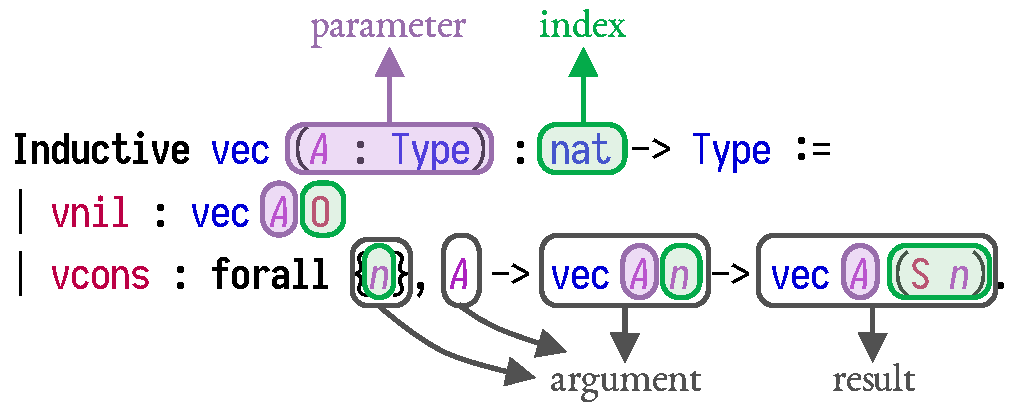
\includegraphics[scale=.59]{figures/inductive.pdf}
\centering
\caption{The definition of the \ty{vec} type in Coq.}
\end{figure}

% \begin{Verbatim}
% \kw{Inductive} \ty{vec} (\bn{A} : \ty{Type}) : \ty{nat} -> \ty{Type} :=
% | \dt{vnil} : \ty{vec} \bn{A} \dt{O}
% | \dt{vcons} : \kw{forall} \bn{n}, \bn{A} -> \ty{vec} \bn{A} \bn{n} -> \ty{vec} \bn{A} (\dt{S} \bn{n}).
% \end{Verbatim}

The code above defines a type \vec{} with two \emph{\glspl{data constructor}}: \vnil{} and \vcons{}. While \vec{} is the name of the inductive type, it doesn't have the type \ty{Type}, unlike a type like \ty{nat}. This is because \vec{} itself needs to take arguments. In other words, \vec{} is a \emph{\gls{type constructor}}. When the word ``constructor" is used alone, it refers to data constructors. The term ``\gls{data constructor}" is only used in contrast to type constructors.

The first of \vec{}’s arguments is an example of a \emph{\gls{parameter}}, and the second is an example of an \emph{\gls{index}}~\cite{dybjer1994}. Both \gls{parameter}s and \glslink{index}{indices} are arguments to the return type of the \gls{inductive type}. \Gls{parameter}s are written before the colon in the type signature of the \gls{inductive type} being defined, while indices come after. \Gls{parameter}s must remain consistent across all constructors' return types, while indices can vary. It is worth noting that all the return types in \vec{} have \bn{A} as the first argument, but the second argument varies between \dt{O} or \Verb|\dt{S} \bn{n}|. Thanks to this variation, the \vec{} type can be indexed with different list lengths.

Notice that \vnil{} takes no arguments, whereas \vcons{} takes three. The first argument that \vcons{} takes is named \bn{n}, while the other two arguments remain unnamed. This argument is named because the return type depends on it, whereas no type depends on the other two arguments. The type of this argument, \ty{nat}, can be omitted here since the type checker can infer it based on the type of \vec{}.

\paragraph*{Implicit and Explicit Arguments} The curly braces around \bn{n}, the first argument of \vcons{}, tell the Coq type checker that this argument is \emph{implicit}, which means this argument will be skipped in a normal application of \vcons{}, and the Coq type checker will try to infer it depending on the context.

\vspace{.2in}
\begin{SaveVerbatim}{E}
\kw{Check} \dt{vcons}.
\end{SaveVerbatim}
\tocoq{\UseVerbatim{E}}

\begin{SaveVerbatim}{E}
\dt{vcons}
     : \bn{?A} -> \ty{vec} \bn{?A} \bn{?n} -> \ty{vec} \bn{?A} (\dt{S} \bn{?n})
\kw{where}
\bn{?A} : [ |- \ty{Type}]
\bn{?n} : [ |- \ty{nat}]
\end{SaveVerbatim}
\fromcoq{\UseVerbatim{E}}

By adding \code{@} in front of a function or inductive type name, we can turn all implicit arguments in the type into explicit arguments:

\vspace{.2in}
\begin{SaveVerbatim}{E}
\kw{Check} @\dt{vcons}.
\end{SaveVerbatim}
\tocoq{\UseVerbatim{E}}

\begin{SaveVerbatim}{E}
@\dt{vcons}
     : \kw{forall} (\bn{A} : \ty{Type}) (\bn{n} : \ty{nat}), \bn{A} -> \ty{vec} \bn{A} \bn{n} -> \ty{vec} \bn{A} (\dt{S} \bn{n})
\end{SaveVerbatim}
\fromcoq{\UseVerbatim{E}}


\paragraph*{Inspecting Inductive Values}

Values of \gls{inductive type}s can be inspected by \kw{match} expressions. The programmer can write functions that contain \kw{match} expressions (and ones that do not) using the \kw{fun} keyword in \gls{Gallina} or the \kw{Definition} keyword in \gls{Vernacular}, as we have seen in the \listsum{} example. Recursive functions, however, need to be defined using the \kw{fix} keyword in \gls{Gallina} or the \kw{Fixpoint} keyword in \gls{Vernacular}:

\begin{Verbatim}
\kw{Fixpoint} \fn{vlength} \{\bn{A} : \ty{Type}\} \{\bn{n} : \ty{nat}\} (\bn{xs} : \vec{} \bn{A} \bn{n}) \{\kw{struct} \bn{xs}\} : \ty{nat} :=
  \kw{match} \bn{xs} \kw{with}
  | \vnil{} => \dt{O}
  | \vcons{} \bn{x} \bn{xs'} => \dt{S} (\fn{vlength} \bn{xs'})
  \kw{end}.

\kw{Definition} \fn{vmap} :=
  \kw{fix} \fn{vmap} \{\bn{A} \bn{B} : \ty{Type}\} \{\bn{n} : \ty{nat}\} 
           (\bn{f} : \bn{A} -> \bn{B}) (\bn{xs} : \vec{} \bn{A} \bn{n}) \{\kw{struct} \bn{xs}\} : \vec{} \bn{B} \bn{n} :=
    \kw{match} \bn{xs} \kw{with}
    | \vnil{} => \vnil{}
    | \vcons{} \bn{x} \bn{xs'} => \vcons{} (\bn{f} \bn{x}) (\fn{vmap} \bn{f} \bn{xs'})
    \kw{end}.
\end{Verbatim}

Here, we define two recursive functions. The first function, \fn{vlength} computes the length of a \vec{}. The second function, \fn{vmap} transforms all the elements of a \vec{} by applying the higher-order function \bn{f}.

In these examples, \fn{vlength} is defined using \kw{Fixpoint}, and \fn{vmap} is defined using \kw{fix}. In practice, top-level recursive functions are usually defined using \kw{Fixpoint}. The \kw{fix} syntax is usually reserved for when we have to write or generate \gls{Gallina} terms, or when we have to define recursive auxiliary functions within other functions.

\section{Metaprogramming Facilities}

A simple definition of \gls{metaprogramming} is the generation or analysis of programs by other programs. By this broad definition, C macros~\cite{stallman1987c} are \gls{metaprogramming}, JavaScript's \fn{eval} is \gls{metaprogramming}, even replacing text in code before compilation counts as \gls{metaprogramming}. \Gls{metaprogramming} comes in many different shapes and colors. 

In this thesis, we will use MetaCoq, a homogeneous generative \gls{metaprogramming}~\cite{hgmp} system for Coq, and \gls{Ltac}, a tactic language for Coq proofs. We will also later develop our own \gls{metaprogramming} abstractions that are based on these two systems.

\subsection{MetaCoq}
\label{metacoq}
MetaCoq is a project formalizing Coq in Coq, and it comes with a quoting mechanism for Coq~\cite{templatecoq, sozeau2020metacoq}. It provides \gls{primitive}s in Coq that can use and manipulate \gls{Gallina} terms and types based on a deeply embedded description of \gls{Gallina} terms, which can also be viewed as abstract syntax trees of \gls{Gallina} terms within \gls{Gallina}.

Here we see an example of a \emph{\gls{quotation}}, i.e. converting an expression into a deeply embedded description, i.e. the \ty{term} type in MetaCoq. 

% \kw{Check} <% \dt{true} %>.
\vspace{.2in}
\begin{SaveVerbatim}{E}
\kw{MetaCoq Run} (\fn{tmQuote} \dt{true} \fn{>>}\fn{=} \fn{tmPrint}).
\end{SaveVerbatim}
\tocoq{\UseVerbatim{E}}

\begin{SaveVerbatim}{E}
\dt{tConstruct}
  \{| \fn{inductive_mind} := (\dt{MPfile} [\dt{"Datatypes"}; \dt{"Init"}; \dt{"Coq"}], \dt{"bool"})
   ; \fn{inductive_ind} := \dt{0} |\} \dt{0} \dt{[]} : \ty{term}
\end{SaveVerbatim}
\fromcoq{\UseVerbatim{E}}

The description of the term \dt{true} above tells us that \dt{true} is the zeroth constructor of the type \ty{bool}, which is located in the \code{\ty{Coq}.\ty{Init}.\ty{Datatypes}} module.

For top-level quotations, we often use the \code{<\% ... \%>} syntax, defined as a simple Coq notation using the primitive tactic from MetaCoq:

\vspace{.2in}
\begin{SaveVerbatim}{E}
\kw{Check} <\% \fn{andb} \%>.
\end{SaveVerbatim}
\tocoq{\UseVerbatim{E}}

\begin{SaveVerbatim}{E}
\dt{tConst} (\dt{MPfile} \dt{[}\dt{"Datatypes"}; \dt{"Init"}; \dt{"Coq"}\dt{]}, \dt{"andb"}) \dt{[]})
  : \ty{term}
\end{SaveVerbatim}
\fromcoq{\UseVerbatim{E}}

The description of the term \fn{andb} tells us that \fn{andb} is a constant definition that is located in the \code{\ty{Coq}.\ty{Init}.\ty{Datatypes}} module.

Here is an example of an \emph{\gls{unquotation}} (also called \emph{antiquotation} or \emph{splice} in the literature), converting a deeply embedded description into an expression.
We have the \ty{term} description of the variable referring to the logical ``and'' operator for Boolean values. By unquoting it, we can obtain the actual \fn{andb} function.

\vspace{.2in}
\begin{SaveVerbatim}{E}
\kw{MetaCoq Run} (\fn{tmUnquoteTyped} _ 
               (\dt{tConst} (\dt{MPfile} \dt{[}\dt{"Datatypes"}; \dt{"Init"}; \dt{"Coq"}\dt{]}, \dt{"andb"}) \dt{[]})
             \fn{>>}\fn{=} \fn{tmPrint}).
\end{SaveVerbatim}
\tocoq{\UseVerbatim{E}}

\begin{SaveVerbatim}{E}
\fn{andb}
\end{SaveVerbatim}
\fromcoq{\UseVerbatim{E}}

For top-level unquotations, we often use the \code{\~{}( ... )} syntax, defined as a simple Coq notation using the primitive tactic from MetaCoq.


\newcommand{\TemplateMonad}{\hyperref[code:TemplateMonad]{\ty{TemplateMonad}}}
This is quite similar to systems like untyped\footnote{A template \gls{metaprogramming} system makes \emph{code fragments} first-class values. An \emph{untyped} template \gls{metaprogramming} system would give these code fragments the same type, such as the \ty{term} type in MetaCoq or the \ty{Exp} type in Template Haskell. A \emph{typed} template \gls{metaprogramming} system would give code fragments types based on the code in the fragment, such as \code{.<\dt{1}\fn{+}\dt{2}>. : \ty{int code}} in MetaML~\cite{taha2000metaml}.} Template Haskell (TH)~\cite{sheard2002template}. Both systems have a deeply embedded description type for expressions (\ty{Exp} for TH and \ty{term} for MetaCoq), a monadic interface for primitive actions (\ty{Q} for TH and \TemplateMonad\label{code:TemplateMonad} for MetaCoq), and a language primitive to run them (\code{\$(...)} splicing in TH and the \kw{MetaCoq Run} \gls{Vernacular} command in MetaCoq).

The primary features of MetaCoq we use are
\begin{enumerate}[nosep]
\item generating terms
\item generating definitions and type class instances
\item generating proof obligations
\item inspecting inductive types
\end{enumerate}
and we want to show examples of these in this section.


\paragraph*{Generating Terms}

Let us start with generating terms. The classic example of generative \gls{metaprogramming} systems is generating a specialized power function~\cite{sheard2001, taha2004, coutts2004, rompf2012, stucki2018}. This example is useful for illustrating the capabilities of a typed \gls{metaprogramming} system, and how well it can handle quasiquoting and scoping. As of the time this thesis is written, a dependently typed MetaML-style \gls{metaprogramming} system is an active research area and an unsolved problem for a full language~\cite{kawata2019dependently, xie2022staging}.


In the most naive form, you would write the power function as such:
\begin{Verbatim}
\kw{Fixpoint} \fn{naive_pow} (\bn{exponent} : \ty{nat}) (\bn{base} : \ty{nat}) : \ty{nat} :=
  \kw{match} \bn{exponent} \kw{with}
  | \dt{0} => \dt{1}
  | \dt{S} \bn{exponent'} => \bn{base} * \fn{naive_pow} \bn{exponent'} \bn{base}
  \kw{end}.
\end{Verbatim}

Observe that this function is recursive, but not tail recursive. One way we can use MetaCoq to optimize it to generate a power function specialized to its exponent. Such a function would allow us to have a non-recursive power function for a fixed exponent, such as \linebreak\code{\kw{fun} \bn{x} => \bn{x} \fn{*} (\bn{x} \fn{*} \bn{x})} that takes a number to its 3rd power. Here is a function that produces the deeply embedded description of such a function, given an exponent:

\newcommand{\makespecializedpow}{\hyperref[code:makespecializedpow]{\fn{make\_specialized\_pow}}}
\label{code:makespecializedpow}
\begin{Verbatim}
\kw{Definition} \makespecializedpow (\bn{exponent} : \ty{nat}) : \ty{term} :=
  \kw{let} \kw{fix} \bn{aux} (\bn{exponent} : \ty{nat}) (\bn{base} : \ty{term}) : \ty{term} :=
    \kw{match} \bn{exponent} \kw{with}
    | \dt{0} => <% \dt{1} %>
    | \dt{S} \bn{exponent'} => \dt{tApp} <% \fn{Nat.mul} %> [\bn{base}; \bn{aux} \bn{exponent'} \bn{base}]
    \kw{end}
  \kw{in} \dt{tLambda} \{| \fn{binder_name} := \dt{nNamed} \dt{"n"}; \fn{binder_relevance} := \dt{Relevant} |\}
             <% \ty{nat} %>
             (\bn{aux} \bn{exponent} (\dt{tRel} \dt{0})).
\end{Verbatim}


Now we can call the specialized power function generator with a specific exponent, \unquote{} the result, and observe the generated function term:

\vspace{.2in}
\begin{SaveVerbatim}{E}
\kw{Check} ~(\makespecializedpow{} \dt{3}).
\end{SaveVerbatim}
\tocoq{\UseVerbatim{E}}

\begin{SaveVerbatim}{E}
\kw{fun} \bn{n} : \ty{nat} => \bn{n} \fn{*} (\bn{n} \fn{*} (\bn{n} \fn{*} \dt{1})) : \ty{nat} -> \ty{nat}
\end{SaveVerbatim}
\fromcoq{\UseVerbatim{E}}

Notice that this specialized power function cubes the input nonrecursively, unlike the \fn{naive\_pow} function. Therefore, our initial goal has been achieved.

\paragraph*{Generating Definitions and Type Class Instances}

The function term generated by \makespecializedpow{} is not made into a definition yet. Ideally, the programmer would generate a definition specialized for a particular exponent and reuse it. Now, let us generate a definition using MetaCoq.

\begin{Verbatim}
\kw{Definition} \fn{generate_specialized_pow} (\bn{exponent} : \ty{nat}) : \TemplateMonad{} \ty{unit} :=
  \bn{name} <- \fn{tmFreshName} (\fn{append} \dt{"pow"} (\fn{string_of_nat} \bn{exponent})) ;;
  \bn{fn} <- \fn{tmUnquoteTyped} (\ty{nat} -> \ty{nat}) (\makespecializedpow{} \bn{exponent}) ;;
  \fn{tmDefinition} \bn{name} \bn{fn} ;;
  \fn{ret} \dt{tt}.
\end{Verbatim}

This function takes an exponent, such as 3, and generates a function named \fn{pow3}, defined as the function term generated by \makespecializedpow{} above:

\vspace{.2in}
\begin{SaveVerbatim}{E}
\kw{MetaCoq Run} (\fn{generate_specialized_pow} \dt{3}).
\kw{Compute} (\fn{pow3} \dt{2}).
\end{SaveVerbatim}
\tocoq{\UseVerbatim{E}}

\begin{SaveVerbatim}{E}
\dt{8} : \ty{nat}
\end{SaveVerbatim}
\fromcoq{\UseVerbatim{E}}

In this thesis, we will use Coq's type classes~\cite{sozeau2008first} as a way of organizing generated data, therefore it is useful to see an example use of MetaCoq with type classes.

Type classes, as defined in Haskell literature, usually are indexed by other types, and they are used for overloading a single function name for different types. Type classes in Coq are built upon dependent records. Like \gls{inductive type}s, they can have any kind (not just types) of \gls{parameter}s.
Here we can overload a single function name for different \ty{nat}s used as fixed exponents.

\begin{Verbatim}
\kw{Class} \ty{Pow} (\bn{exponent} : \ty{nat}) : \ty{Type} :=
  \{ \fn{pow} : \kw{forall} (\bn{base} : \ty{nat}), \ty{nat} \}.

\kw{Instance} \fn{Pow2} : \ty{Pow} \dt{2} := \{| \fn{pow} := ~(\makespecializedpow{} \dt{2}) |\}.

\kw{Definition} \fn{special_pow} (\bn{exponent} : \ty{nat}) `\{\ty{Pow} \bn{exponent}\} (\bn{base} : \ty{nat}) : \ty{nat} :=
  @\fn{pow} \bn{exponent} _ \bn{base}.
\end{Verbatim}

Here we define a type class that is parametrized by the exponent, which is a \ty{nat}, and then we write instances of this type class for each fixed exponent we want to specialize for.
Then we define the \fn{special\_pow} helper function, which makes the exponent argument explicit, but the type class instance implicit.
Now we can call this function to get the square of a number:

\newpage
\vspace{.2in}
\begin{SaveVerbatim}{E}
\kw{Compute} (\fn{special_pow} \dt{2} \dt{3}).
\end{SaveVerbatim}
\tocoq{\UseVerbatim{E}}

\begin{SaveVerbatim}{E}
\dt{9} : \ty{nat}
\end{SaveVerbatim}
\fromcoq{\UseVerbatim{E}}

Ideally, we would not have to write the instances of the \ty{Pow} type class by hand, so let us utilize MetaCoq to generate them automatically up to a certain exponent:

\newcommand{\generatepowinstance}{\hyperref[code:generatepowinstance]{\fn{generate\_pow\_instance}}}
\newcommand{\generatepowinstances}{\hyperref[code:generatepowinstances]{\fn{generate\_pow\_instances}}}
\label{code:generatepowinstance}
\label{code:generatepowinstances}
\begin{Verbatim}
\kw{Definition} \generatepowinstance (\bn{exponent} : \ty{nat}) : \TemplateMonad{} \ty{unit} :=
  \bn{name} <- \fn{tmFreshName} (\fn{append} \dt{"Pow"} (\fn{string_of_nat} \bn{exponent})) ;;
  \bn{fn} <- \fn{tmUnquoteTyped} (\ty{nat} -> \ty{nat}) (\makespecializedpow{} \bn{exponent}) ;; 
  @\fn{tmDefinition} \bn{name} (\ty{Pow} \bn{exponent}) \{| \fn{pow} := \bn{fn} |\} ;;
  \bn{mp} <- \fn{tmCurrentModPath} \dt{tt} ;;
  \fn{tmExistingInstance} \dt{export} (\dt{ConstRef} (\bn{mp}, \bn{name})).

\kw{Fixpoint} \generatepowinstances (\bn{exponent} : \ty{nat}) : \TemplateMonad{} \ty{unit} :=
  \generatepowinstance{} \bn{exponent} ;;
  \kw{match} \bn{exponent} \kw{with}
  | \dt{O} => \fn{ret} \dt{tt}
  | \dt{S} \bn{exponent'} => \generatepowinstances{} \bn{exponent'}
  \kw{end}.
\end{Verbatim}

The first function generates an instance for a particular exponent, while the second one generates instances for all natural numbers less than or equal to the one it starts from. Here is an example use:

\vspace{.2in}
\begin{SaveVerbatim}{E}
\kw{MetaCoq Run} (\generatepowinstances{} \dt{5}).
\kw{Compute} (\fn{special_pow} \dt{4} \dt{2}).
\end{SaveVerbatim}
\tocoq{\UseVerbatim{E}}

\begin{SaveVerbatim}{E}
\dt{16} : \ty{nat}
\end{SaveVerbatim}
\fromcoq{\UseVerbatim{E}}

Remember that this will only work if there is a \ty{Pow} instance for the particular exponent we want to use. If there is no such instance, the \ty{Pow} instance will remain an unsolved existential variable.

\paragraph*{Generating Proof Obligations}

As you can observe in the \makespecializedpow{} function, term generation with MetaCoq can be quite verbose. This is due to MetaCoq's design: MetaCoq reifies terms as they are in the core language of Coq, where all syntactic sugar has already disappeared. In the core language, there are no notations, records have become inductive types, and implicit arguments have become explicit. Therefore all generated code has to be verbose core-language code. This gets especially tricky when we are generating complicated proofs. At times like this, \gls{Ltac} is a more useful tool for generating proofs. Therefore, we use the feature of MetaCoq that creates obligations.

To set up an example for this feature, let us revise the \ty{Pow} type class and add a field stating that the specialized power function has to return the same result as the naive power function:

\begin{Verbatim}
\kw{Class} \ty{Pow} (\bn{exponent} : \ty{nat}) : \ty{Type} :=
  \{ \fn{pow} : \kw{forall} (\bn{base} : \ty{nat}), \ty{nat}
  ; \fn{eq_naive} : \kw{forall} (\bn{base} : \ty{nat}), \fn{pow} \bn{base} \ty{=} \fn{naive_pow} \bn{exponent} \bn{base}
  \}.
\end{Verbatim}

Now we will have to update the \generatepowinstance{} function to generate the \fn{eq\_naive} field as well. In order to avoid generating this proof with the core language terms with MetaCoq, we can discharge this term as an obligation and later use \gls{Ltac} to satisfy that obligation.

\newcommand{\tmLemma}{\hyperref[code:tmLemma]{\fn{tmLemma}}}
\begin{Verbatim}
\kw{Definition} \fn{generate_pow_instance} (\bn{exponent} : \ty{nat}) : \TemplateMonad{} \ty{unit} :=
  \bn{name} <- \fn{tmFreshName} (\fn{append} \dt{"Pow"} (\fn{string_of_nat} \bn{exponent})) ;;
  \bn{fn} <- \fn{tmUnquoteTyped} (\ty{nat} -> \ty{nat}) (\makespecializedpow{} \bn{exponent}) ;;
  \bn{eq_name} <- \fn{tmFreshName} (\fn{append} \dt{"eq"} (\fn{string_of_nat} \bn{exponent})) ;;
  \bn{lem} <- \tmLemma{}\label{code:tmLemma} \bn{eq_name} _ ;;
  @\fn{tmDefinition} \bn{name} (\ty{Pow} \bn{exponent}) \{| \fn{pow} := \bn{fn} ; \fn{eq_naive} := \bn{lem} |\} ;;
  \bn{mp} <- \fn{tmCurrentModPath} \dt{tt} ;;
  \fn{tmExistingInstance} \dt{export} (\dt{ConstRef} (\bn{mp}, \bn{name})).

\kw{Obligation Tactic} := \fn{auto}.
\end{Verbatim}

Here we used \tmLemma{} to create the proof obligation of a certain type (left as \code{\_} in the code but inferred by the type checker), and later the \fn{auto} tactic from \gls{Ltac} solves the proof obligation.

Now we can call \generatepowinstances{} as usual and generate all the \ty{Pow} instances we need.

\paragraph*{Inspecting Inductive Types}

The final feature of MetaCoq that we use a lot in this thesis is inspecting an inductive type. Given a term, we can ask MetaCoq to give a detailed description of the inductive types that are used in the term:

\newcommand{\tmQuoteRec}{\hyperref[code:tmQuoteRec]{\fn{tmQuoteRec}}}
\vspace{.2in}
\begin{SaveVerbatim}{E}
\kw{MetaCoq Run} (\tmQuoteRec{}\label{code:tmQuoteRec} \ty{nat} \fn{>>}\fn{=} \fn{tmPrint}).
\end{SaveVerbatim}
\tocoq{\UseVerbatim{E}}

\begin{SaveVerbatim}{E}
(\{| ...
   \fn{declarations} :=
     \dt{[}((\dt{MPfile} \dt{["Datatypes"}; \dt{"Init"}; \dt{"Coq"}\dt{]}, \dt{"nat"}),
       \dt{InductiveDecl} \{| ...
         ; \fn{ind_params} := \dt{[]}
         ; \fn{ind_bodies} := 
             \dt{[}\{| \fn{ind_name} := \dt{"nat"} ; ...
               ; \fn{ind_ctors} := 
                   \dt{[}\{| \fn{cstr_name} := \dt{"O"}
                     ; \fn{cstr_args} := \dt{[]} ; \fn{cstr_indices} := \dt{[]}
                     ; \fn{cstr_type} := \dt{tRel} \dt{0} ; \fn{cstr_arity} := \dt{0} |\}
                  ; \{| \fn{cstr_name} := \dt{"S"}
                     ; \fn{cstr_args} :=
                         \dt{[}\{| \fn{decl_name} := \{| \fn{binder_name} := \dt{nAnon}
                                           ; \fn{binder_relevance} := \dt{Relevant} |\}
                           ; \fn{decl_body} := \dt{None}
                           ; \fn{decl_type} := \dt{tRel} \dt{0} |\}\dt{]}
                     ; \fn{cstr_indices} := \dt{[]}
                     ; \fn{cstr_type} :=
                         \dt{tProd} \{| \fn{binder_name} := \dt{nAnon}
                                ; \fn{binder_relevance} := \dt{Relevant} |\} 
                          (\dt{tRel} \dt{0}) (\dt{tRel} \dt{1})
                     ; \fn{cstr_arity} := \dt{1} |\}\dt{]}
               ; \fn{ind_projs} := \dt{[]} ; \fn{ind_relevance} := \dt{Relevant} |\}\dt{]} |\})\dt{]} |\},
 \dt{tInd} \{| \fn{inductive_mind} := (\dt{MPfile} \dt{["Datatypes"}; \dt{"Init"}; \dt{"Coq"}\dt{]}, \dt{"nat"})
       ; \fn{inductive_ind} := \dt{0} |\} \dt{[])}
\end{SaveVerbatim}
\fromcoq{\UseVerbatim{E}}

% \newpage
\label{inspecting-inductive-types}

Here we see the description MetaCoq gives, simplified for presentation. We see a mutually \gls{inductive type} block, in which we only have one type. We can access the \gls{parameter}s of the block, types, arguments, names, \indices{} of each \constructor. This covers almost all the information from MetaCoq that we use in our code generation.


\subsection{Ltac}\label{ltac}
\gls{Ltac} is a domain-specific language for proofs and decision procedures in Coq. \gls{Ltac} allows the user to manipulate the proof state imperatively, through commands called \emph{tactics}. Tactics change the \emph{proof state}, which includes the goals and the context. In an interactive Coq session, the user can step forward or backward to see exactly how a tactic changes the proof state. Tactics can add to or remove from the context. Tactics can create new goals. Tactics can satisfy goals. \gls{Ltac} generates a proof term in \gls{Gallina} when all the goals are satisfied.

Most of the attention in the \gls{metaprogramming} literature is directed at homogeneous \gls{metaprogramming}, where the \glslink{object language}{object} and \gls{meta language}s are the same. Template Haskell~\cite{sheard2002template} and MetaML~\cite{taha2000metaml} are the most prominent examples of this among typed functional languages. MetaCoq's quoting mechanism is the Coq equivalent of this tradition~\cite{templatecoq}.
\gls{Ltac}, although usually not classified as a \gls{metaprogramming} language, deserves to be classified as such, only a heterogeneous one, where the object language is \gls{Gallina} and the meta language is \gls{Ltac} ~\cite{bergerSlides}.

\gls{Ltac} can inspect \gls{Gallina} terms and generate new \gls{Gallina} terms. It operates on the surface syntax of \gls{Gallina} rather than a deeply embedded representation of \gls{Gallina}. MetaCoq, on the other hand, operates on the deeply embedded representation of the core language. Here is an example that inspects a term and creates a new term, presented in both \gls{Ltac} and MetaCoq for comparison:

\begin{Verbatim}
\kw{Ltac} \tc{single_app_tac} \bn{t} :=
  \kw{match} \bn{t} \kw{with}
  | \bn{?f} _ => \kw{let} \bn{x} := (\kw{constr:}(\bn{f t})) \kw{in} \tc{idtac} \bn{x}
  | _ => \tc{fail}
  \kw{end}.

\kw{Definition} \fn{single_app_fn} {\bn{A} : \ty{Type}} (\bn{a} : \bn{A}) : \TemplateMonad{} \ty{unit} :=
  \bn{t} <- \fn{tmQuote} \bn{a} ;;
  \kw{match} \bn{t} \kw{with}
  | \dt{tApp} \bn{f} \dt{[}_\dt{]} => \fn{tmPrint} (\dt{tApp} \bn{f} \dt{[}\bn{t}\dt{]})
  | _ => \fn{tmFail} \dt{""}
  \kw{end}.
\end{Verbatim}

Both the \gls{Ltac} tactic and the MetaCoq function check if a given \gls{Gallina} term is an application. If it is, then the result is a new term that is the same function applied to the original term, and this result is printed. If the term is not an application, then the tactic or the function fails. This tactic can be used to turn \dt{S O} into \code{\dt{S} (\dt{S O})}, or to turn \code{\fn{negb} \dt{true}} into \code{\fn{negb} (\fn{negb} \dt{true})}.

\gls{Ltac} allows pattern-matching not only on \gls{Gallina} terms but also on the context of the proof. It allows checking if a given name, or a value whose type fits a certain pattern, is in the context. Similarly, \gls{Ltac} can pattern-match on the goal as well:

\begin{Verbatim}
\kw{Ltac} \tc{destructs} :=
  \tc{match goal} \kw{with}
  | [ \bn{x} : _ \ty{*} _ |- _ ] =>
      \kw{let} \bn{p1} := \tc{fresh} \dt{"p"} \kw{in}
      \kw{let} \bn{p2} := \tc{fresh} \dt{"p"} \kw{in}
      \tc{destruct} \bn{x} \tc{as} [\bn{p1 p2}]; \tc{destructs}
  | [ |- _ \ty{*} _ ] => \tc{split}; \tc{destructs}
  | _ => \fn{idtac}
  \kw{end}.
\end{Verbatim}

This tactic does two different things: If there are any pairs in the context, it \tc{destruct}s them, i.e. adds the projections of the pair fields to the context (with fresh names) and removes the original pair from the context, and recurses to handle any nested pairs that may occur in the projections. The second thing the tactic does is to check if the goal is a pair as well, and \tc{split} that goal into two subgoals, one for each field of the pair, and then it recurses to handle any nested pairs. The tactic stops when there are no pairs in the context or the goal.

In the thesis, we will use \gls{Ltac}'s ability to match on goals to pass information from MetaCoq to \gls{Ltac}. In \autoref{ctordesc}, we will see that we can create a goal type that is a function call with an unused argument, where we can pattern match on the unused argument and use it in \gls{Ltac}.

\gls{Ltac} unfortunately does not let us inspect the constructors of an inductive type. While it is possible to use tactics like \tc{case} or \tc{induction} on a value of a given type, and that can give us some information about the arguments of a constructor, it is not possible to get a general look over all the constructors of an inductive type, since that would require the ability to consider multiple subgoals at the same time, which is not possible. However, \gls{Ltac} provides the ability to apply a constructor that fits the type of the goal. Using tactics like \tc{constructor} (or \tc{unshelve econstructor} to deal with existential variables), the user can apply a constructor that fits the goal, without having to pattern-match on the goal type, or without having to know what the constructors of the goal type are.

% Both in Ltac and MetaCoq, the term represented in the syntax is untyped, but the entry and exit points are type-checked by the Coq type-checker. In other words, 


% This would have allowed %TODO



% The surface syntax %TODO


% This has both positive and negative consequences.
% The positive one is that this allows 

% which is limiting how much information can be generated or inspected, 
% It is limiting because 

% Ltac does not work based on a deeply embedded representation of Gallina terms, 
% Ltac tactics can contain Gallina terms, but it has other metaprogramming capabilities, such as matching on patterns before evaluation or applying constructors without naming them. 


% When we want to talk about terms of a language in the language itself, we need a way to represent any term in the same language. 

\chapter{The Foreign Function Interface}
\label{usage}

\epigraph{Since large programs grow from small ones, it is crucial that we develop an arsenal of\\ standard program structures of whose correctness we have become sure—we call them idioms—\\and learn to combine them into larger structures using organizational techniques of proven value.}{Alan J. Perlis~\cite{abelson1996structure}}


In this chapter, we will showcase a simple use case of CertiCoq's foreign function interface and examine the glue code generated by CertiCoq.

For pedagogical purposes, this chapter discusses implementing in C what one could have also implemented in Coq (though less efficiently), but later chapters describe foreign functions that could not be implemented in Coq.

The Coq code described in this chapter uses \gls{Vernacular} commands that are defined in the CertiCoq plugin, namely \kw{CertiCoq Register}, \kw{CertiCoq Compile}, and \kw{CertiCoq Generate Glue} commands. In order to be able to run these \gls{Vernacular} commands, you would have to have a CertiCoq installation on your machine or in your container.

\section{An Example Use of the Interface}
Suppose we want to have a hand-optimized implementation of a Coq function. Take the \fn{div2} function from the Coq standard library. This function divides a natural number by 2.

\begin{Verbatim}
\kw{Fixpoint} \fn{div2} (\bn{n} : \ty{nat}) :=
  \kw{match} \bn{n} \kw{with}
  | \dt{S} (\dt{S} \bn{n'}) => \dt{S} (\fn{div2} \bn{n'})
  | _ => \dt{0}
  \kw{end}.
\end{Verbatim}

Notice that \fn{div2} is not tail recursive, and it allocates memory for the constructor \dt{S} before every recursive call. Hence this function is not memory and stack-space efficient. It is possible to write a more efficient version of this function with tail recursion and no memory allocations:

\begin{Verbatim}
\kw{Definition} \fn{better_div2} (\bn{n} : \ty{nat}) : \ty{nat} :=
  \kw{let fix} \fn{aux} (\bn{n} \bn{m} : \ty{nat}) : \ty{nat} :=
    \kw{match} \bn{n} , \bn{m} \kw{with}
    | \dt{S} \bn{n'}, \dt{S} (\dt{S} \bn{m'}) => \fn{aux} \bn{n' m'}
    | \dt{S} \bn{n'}, \dt{1} => \bn{n'}
    | _, _ => \bn{n}
    \kw{end}
  \kw{in} \fn{aux} \bn{n n}.
\end{Verbatim}

To achieve optimal performance, CertiCoq compiles this function into a tail-recursive C function. This C function can then be further optimized into a loop by smart C compilers like CompCert, GCC, or Clang at higher optimization levels. In fact, both GCC and Clang can generate code that is comparable to hand-written C code for this function. 
% However, if we need to use CompCert or if we have to use lower optimization levels due to other reasons (e.g., if our unverified C compiler occasionally produces buggy output at higher optimization levels), we can take a different approach. We can declare the function as a foreign function in Coq and implement it in C.
However, we will show a different approach to compile more complex and compute-intensive functions, such as cryptographic primitives that could benefit from using C primitives such as arrays and bit-level arithmetic  \cite{appel2015sha256}. For simplicity, we will continue to use \fn{div2} as a pedagogical example.

To be able to call our function, we have to create an object on the Coq side. We follow Coq's traditional program extraction mechanism here and ask the user to declare the function as an axiom, which will be realized later when we compile our program.

\begin{Verbatim}
\kw{Axiom} \fn{best_div2} : \ty{nat} -> \ty{nat}.
\end{Verbatim}

Once we declare the axiom, we can tell the compiler that this axiom will be realized by a C function, and where that C function lives. This is achieved through the \kw{CertiCoq Register} command:

\begin{Verbatim}
\kw{CertiCoq} \kw{Register} [ \fn{best_div2} => \dt{"best_div2"} ] \kw{Include} [ \dt{"prims.h"} ].
\end{Verbatim}

Now we can declare our C function in a C header file:

\begin{Verbatim}
\ty{value} \fn{best_div2}(\ty{value});
\end{Verbatim}

CertiCoq represents Coq values in memory in a uniform way, as we will describe in greater detail in \autoref{memoryrepresentation}. We have the C type \ty{value} that all Coq values, regardless of their types, live in. In other words, \ty{value} is the C type of Coq values represented in C. The arguments and the result of our function, when realized in C, will all have the C type \ty{value}.

Finally, we can implement our function in a C source file:

\begin{Verbatim}
\ty{value} \fn{best_div2}(\ty{value} \bn{a}) \{
  \ty{value} \bn{tortoise} = \bn{a}, \bn{hare} = \bn{a};
  \cm{/* All these function calls will be inlined by the compiler, of course. */}
  \kw{while} (\fn{get_Coq_Init_Datatypes_nat_tag}(\bn{hare}) \fn{=}\fn{=} \dt{1}) \{
    \bn{tortoise} = \fn{get_args}(\bn{tortoise})[\dt{0}];
    \bn{hare} = \fn{get_args}(\bn{hare})[\dt{0}];
    \kw{if} (\fn{get_Coq_Init_Datatypes_nat_tag}(\bn{hare}) \fn{=}\fn{=} \dt{1}) \{
      \bn{hare} = \fn{get_args}(\bn{hare})[\dt{0}];
    \} \kw{else} \{
      \kw{break};
    \}
  \}
  \kw{return} \bn{tortoise};
\}
\end{Verbatim}

% Our C implementation takes in a Coq value represented in C and outputs a Coq value represented in C.
% Thankfully, a user of CertiCoq's foreign function interface does not have to understand fully how this representation works or what the \ty{value} type is internally; there are functions they can use to interact with \ty{value}s, such as the functions we use in the function above. We refer to these functions collectively as \emph{\gls{glue code}}. We will examine all the functions in glue code automatically generated by CertiCoq in detail in \autoref{glue}.

The C implementation of the function accepts a Coq value represented in C as input and returns a Coq value represented in C as output. Fortunately, users of CertiCoq's foreign function interface do not need to have a deep understanding of the internal workings of the \ty{value} type or how the representation works. CertiCoq provides a set of functions, collectively known as \emph{\gls{glue code}}, that users can use to interact with \ty{value}s, including the functions used in the above function. In the next section (\autoref{glue}), we will examine the details of all the functions automatically generated by CertiCoq in the glue code.

Now we can write a Coq program that uses \fn{best\_div2} and compile it.

\begin{Verbatim}
\kw{Definition} \fn{prog} : \ty{nat} := \fn{best_div2} \dt{5}.
\kw{CertiCoq} \kw{Compile} -file \dt{"prog"} \fn{prog}.
\kw{CertiCoq} \kw{Generate} \kw{Glue} -file \dt{"glue"} [ \ty{nat} ].
\end{Verbatim}

The \kw{CertiCoq Compile} command compiles a program to C but does not print or use the result. The generated program, by default, does not print or use the result either. This differs from other functional languages like Haskell or OCaml. Haskell programs have an effectful program entry point called \fn{main} with the type \ty{IO ()}, which is executed when the program runs. OCaml programs can feature function calls outside of definitions, which run when the program is run, allowing effectful function invocations or an effectful program entry point. CertiCoq programs do not have these, therefore we need to write a C wrapper file to use the result from the Coq code compiled by CertiCoq. This C file serves as the program entry point, one that cannot be written directly in Coq:

\begin{Verbatim}
\kw{#include} \dt{"gc_stack.h"}
\kw{#include} \dt{"glue.h"}
\kw{#include} \dt{"prog.h"}
\end{Verbatim}
\newpage{}

\begin{Verbatim}
\ty{int} \fn{main}() \{
  \kw{struct} \ty{thread_info *}\tinfo{} = \fn{make_tinfo}();
  \ty{value} \bn{result} = \fn{body}(\tinfo{});
  \fn{print_Coq_Init_Datatypes_nat}(\bn{result});
  \kw{return} \dt{0};
\}
\end{Verbatim}

Inside the \fn{main} function, we first create the initial thread information object. Then we call the \fn{body} function, which evaluates the compiled program, namely \fn{prog} in our Coq file. We get the result back and then call a glue code function to print the result. In our case, this program will print \code{(S (S O))}.

The thread information object is a \kw{struct} that contains the necessary information for the CertiCoq runtime to work. This includes the call stack, the location and bounds of the \gls{CertiCoq heap}, and the location of the next allocatable spot in that heap~\cite{belanger2019verified, belanger2019certified, paraskevopoulou2020verified}. We will refer to this object as the \emph{\gls{thread info}}, often abbreviated as \tinfo{} when used as a function argument or a local definition.

Any function that potentially allocates memory in the \gls{CertiCoq heap} must take the \gls{thread info} as an argument. Our foreign C function, \fn{best\_div2}, only inspects Coq values; it does not create new ones. However, if we were to write a version of it that does allocate memory, we would need to declare that to the CertiCoq compiler when registering the foreign function:

\begin{Verbatim}
\kw{CertiCoq} \kw{Register} [ \fn{best_div2} => \dt{"best_div2"} \kw{with tinfo} ] \kw{Include} [ \dt{"prims.h"} ].
\end{Verbatim}

Then the C function type of our foreign function could include the \gls{thread info} as well:

\begin{Verbatim}
\ty{value} \fn{best_div2}(\kw{struct} \ty{thread_info *}\tinfo{}, \ty{value});
\end{Verbatim}

Now that we have reviewed how CertiCoq's foreign function interface is used, let us take a closer look at the glue functions generated by CertiCoq, and how they are implemented.

\section{Generated Glue Code}\label{glue}

The \kw{CertiCoq Generate Glue} command takes a sequence of Coq \gls{inductive type}s and generates corresponding glue functions. For example, if a programmer intends to write foreign functions that interact with Coq \ty{list}s and \ty{nat}s, they would call this command:

\begin{Verbatim}
\kw{CertiCoq} \kw{Generate} \kw{Glue} [ \ty{list} , \ty{nat} ].
\end{Verbatim}

When this vernacular command is run, the compiler generates a file that contains functions in C that programmers can use when writing foreign functions. Here we will explain every kind of function generated in detail, in separate subsections. The functions we will see below will have some syntactic sugar that your compiler output may not have\footnote{This is because when CertiCoq generates C code, it produces Clight code, which is a syntactically restricted subset of C, and then prints it as C code.}, but they are the same functions otherwise.

Generated C functions that are specialized to a particular Coq type will use the fully qualified name of types. For a function that mentions the \ty{list} type by name, the function name will contain \ty{Coq.Init.Datatypes.list} (but with underscores instead of dots), so that name clashes are avoided.

\subsection{Constructing Coq Values}

VeriFFI automatically generates C functions that construct the values for each constructor in each Coq \gls{inductive type} requested by the user. For instance, for the \ty{list} type, VeriFFI generates these functions:\newpage

\newcommand{\makenil}{\hyperref[code:makenil]{\fn{make\_\linebreak[0]Coq\_\linebreak[0]Init\_\linebreak[0]Datatypes\_\linebreak[0]list\_\linebreak[0]nil}}}
\newcommand{\makecons}{\hyperref[code:makecons]{\fn{make\_\linebreak[0]Coq\_\linebreak[0]Init\_\linebreak[0]Datatypes\_\linebreak[0]list\_\linebreak[0]cons}}}
\newcommand{\allocmakecons}{\hyperref[code:allocmakecons]{\fn{alloc\_\linebreak[0]make\_\linebreak[0]Coq\_\linebreak[0]Init\_\linebreak[0]Datatypes\_\linebreak[0]list\_\linebreak[0]cons}}}
\begin{Verbatim}
\ty{value} \makenil{}\label{code:makenil}(\ty{void}) \{
  \kw{return} (\ty{value}) \dt{1};
\}

\ty{value} \makecons{}\label{code:makecons}(\ty{value} \bn{arg0}, \ty{value} \bn{arg1}, \ty{value *}\bn{argv}) \{
  \bn{argv}[\dt{0}] = (\ty{value}) \dt{2048};
  \bn{argv}[\dt{1}] = \bn{arg0};
  \bn{argv}[\dt{2}] = \bn{arg1};
  \kw{return} \bn{argv} \fn{+} \dt{1};
\}

\ty{value} \allocmakecons{}\label{code:allocmakecons}
      (\kw{struct} \ty{thread_info *}\tinfo{}, \ty{value} \bn{arg0}, \ty{value} \bn{arg1}) \{
  \ty{value *}\bn{argv} = \tinfo{}->\bn{alloc};
  \bn{argv}[\dt{0}] = (\ty{value}) \dt{2048};
  \bn{argv}[\dt{1}] = \bn{arg0};
  \bn{argv}[\dt{2}] = \bn{arg1};
  \tinfo{}->\bn{alloc} = \tinfo{}->\bn{alloc} \fn{+} \dt{3};
  \kw{return} \bn{argv} + \dt{1};
\}
\end{Verbatim}

The generated glue function for a constructor can look differently depending on whether it has \gls{boxed} or \gls{unboxed} representation. We provide a more detailed explanation of these representations in \autoref{memoryrepresentation}.
Unboxed constructors, like the \dt{nil} constructor, are represented as integers at runtime. This can be observed in the \makenil{} function.
On the other hand, boxed constructors such as the \dt{cons} constructor, are represented as pointers to memory locations that store the constructor arguments. This memory can exist either within the CertiCoq runtime's garbage-collected memory region, known as the \emph{\gls{CertiCoq heap}}, or outside of it in what we refer to as the \emph{C heap}.
For the \dt{cons} constructor, the \makecons{} function creates a value in the C heap, while the \allocmakecons{} function creates a value in the \gls{CertiCoq heap}.\newpage

When creating a value on the \gls{CertiCoq heap} with the \allocmakecons{} function, we have to pass the \gls{thread info} object so that the glue function knows where to allocate memory. 

When creating a value on the \gls{C heap} with the \makecons{} function, however, we need to pass a pointer to a part of memory, namely \bn{argv}, where the glue function can build a value.
The \bn{argv} pointer must have enough available memory for the function to write on. It requires one word for each \constructor{}, and a word right before the pointer to store header information. It is the programmer's responsibility to free this memory later or keep track of what can be freed and when. The CertiCoq garbage collector does not touch this allocated memory. When allocating on the \gls{C heap}, one must take care of pointers from there into the garbage-collected heap. The CertiCoq garbage collector has mechanisms to manage that, but to avoid such complexity, in this thesis work we have focused mostly on allocation in the \gls{CertiCoq heap}.

\subsection{Discriminating Coq Constructors}

For each Coq \gls{inductive type}, VeriFFI generates a separate C function that allows the user to determine the constructor used to create a value of that type. For example, for the \ty{list} type, the function would be:

\begin{Verbatim}
\ty{unsigned long long} \fn{get_Coq_Init_Datatypes_list_tag}(\ty{value} \bn{v}) \{
  \kw{if} (\fn{is_ptr}(\bn{v})) \{
    \kw{switch} (\fn{get_boxed_ordinal}(\bn{v})) \{
      \kw{case} \dt{0}:
        \kw{return} \dt{1};
    \}
  \} \kw{else} \{
    \kw{switch} (\fn{get_unboxed_ordinal}(\bn{v})) \{
      \kw{case} \dt{0}:
        \kw{return} \dt{0};
    \}
  \}
  \cm{/* In the future, we can add the unreachable() annotation here,}
     \cm{to improve the C compiler's ability to optimize this function. */}
\}
\end{Verbatim}

This function takes a Coq value and returns an integer that matches the word size of your machine, which we call the \emph{\gls{tag}} of the constructor.

A tag is an index (starting from \texttt{0}) denoting the order of the
constructor that was used to create the value at hand. When the C
representation of a Coq value is passed into this function, it returns
\texttt{0} for \dt{nil} and \texttt{1} for \dt{cons}. For
further ease of use, the programmer can define an \kw{enum} type:
\begin{Verbatim}
\kw{typedef} \kw{enum} \{\ \dt{NIL}, \dt{CONS} \}\ \ty{coq\_list};
\end{Verbatim}
The programmer can then treat the result of this function as a value of type \ty{coq\_list}. However, CertiCoq does not generate this type automatically.

Internally, each constructor has an \emph{\gls{ordinal}}, the index of a constructor within the constructors of that \gls{inductive type} with the same \gls{boxity}. Counting the \gls{boxed} and \gls{unboxed} constructors separately is a trick that allows representing a larger number of constructors in the \ty{value} type. However, it is important to note that ordinals are specific to the compiler's implementation and it is not recommended for FFI users to depend on them while writing C code. Instead, it is advisable to use \gls{tag}s and glue functions.

\subsection{Extracting Arguments of a Coq Constructor} 

Given a Coq value of an \gls{inductive type}, we would like to be able to access its \constructor{} arguments. We have a single C function that works on values of any \gls{inductive type}, as long as the value is \gls{boxed}:

\begin{Verbatim}
\ty{value *}\fn{get_args}(\ty{value} \bn{v}) \{
  \kw{return} (\ty{value *}) \bn{v};
\}
\end{Verbatim}

Calling the \fn{get\_args} function on \gls{unboxed} values, \gls{closure}s, or type values will cause undefined behavior at runtime.

\subsection{Printing Coq Values}

For each Coq \gls{inductive type} requested by the user, VeriFFI provides a C function that prints values of that type.
For instance, for the \ty{list} type, this would be:

\begin{Verbatim}
\ty{void} \fn{print_Coq_Init_Datatypes_list}(\ty{value} \bn{v}, \ty{void} \fn{print_param_A}(\ty{value}))
\{
  \ty{unsigned int} \bn{tag};
  \ty{void *}\bn{args};
  \bn{tag} = \fn{get_Coq_Init_Datatypes_list_tag}(\bn{v});
  \kw{switch} (\bn{tag}) \{
    \kw{case} \dt{0}:
      \fn{printf}(\fn{names_of_Coq_Init_Datatypes_list}[\bn{tag}]);
      \kw{break};
    \kw{case} \dt{1}:
      \bn{args} = \fn{get_args}(\bn{v});
      \fn{printf}(\fn{lparen_lit});
      \fn{printf}(\fn{names_of_Coq_Init_Datatypes_list}[\bn{tag}]);
      \fn{printf}(\fn{space_lit});
      \fn{print_param_A}(\fn{get_args}(\bn{args})[\dt{0}]);
      \fn{printf}(\fn{space_lit});
      \fn{print_Coq_Init_Datatypes_list}(\fn{get_args}(\bn{args})[\dt{1}], \fn{print_param_A});
      \fn{printf}(\fn{rparen_lit});
      \kw{break};
  \}
\}
\end{Verbatim}

Notice how since \ty{list} is a parameterized type, the printing function takes a function pointer to deal with values of the parameter type.

\subsection{Calling Coq Closures}

The CertiCoq compiler represents Coq functions as \gls{closure}s at runtime, which consist of a function and an environment, but are not directly callable in C. To call these from C, one must fetch the code-pointer, fetch the environment pointer, and pass the environment as one of the arguments to the code-pointer function.  We have a C function that implements this protocol:

\begin{Verbatim}
\ty{value} \fn{call}(\kw{struct} \ty{thread_info *}\tinfo{}, \ty{value} \bn{clo}, \ty{value} \bn{arg}) \{
  \ty{value} \bn{f} = ((\kw{struct} \ty{closure *}) \bn{clo})->\fn{func};
  \ty{value} \bn{envi} = ((\kw{struct} \ty{closure *}) \bn{clo})->\fn{env};
  \kw{return} ((\ty{value} (\ty{*})(\kw{struct} \ty{thread_info *}, \ty{value}, \ty{value})) \bn{f}) (\tinfo{}, \bn{envi}, \bn{arg});
\}
\end{Verbatim}

When compiling a function definition with CertiCoq, programmers can use the \fn{call} function to pass arguments to it. The \fn{call} function also requires the \gls{thread info} as an argument because functions within \gls{closure}s need the \gls{thread info} to perform memory allocation.

\chapter{Representation Predicates}
\label{predicates}

\epigraph{One might say, by way of excuse, ``but the language in which I program has the kind of address arithmetic that makes it impossible to know the bounds of an array." Yes, and the man who shot\\his mother and father threw himself upon the mercy of the court because he was an orphan.}{Andrew W. Appel~\cite{appel1998modern}}
% page 160 in ML, page 168 in Java. Chapter 7.2

In code compiled from Coq to C by CertiCoq, Coq values are uniformly represented in memory. Foreign C functions called from Coq are expected to take inputs and give outputs in this representation, yet nothing stops them from flouting this expectation. A violation of this representation may cause a runtime error, but there is no way to catch it statically or prove that no such violation exists. In this chapter, I will describe the uniform memory representation of Coq values, I will introduce representation predicates, a mechanism to state the proposition that a Coq value in CertiCoq's heap memory truly represents that value and also respects this uniform representation, unless it is a value of a \gls{foreign type} with a custom representation. I will also describe the automatic generation of representation predicates. 
% And on the other hand, user-defined \gls{foreign type}s (implemented in C) need not have uniform representations, yet they must also fit into this specification framework, as I will explain.\todo{TODO: Did I explain?}

\section{Memory Representation of Values}
\label{memoryrepresentation}

CertiCoq's memory representation of values is almost identical to OCaml's memory representation of values~\cite{madhavapeddy2022real}. This similarity is no coincidence; it was a design choice that is meant to provide compatibility with OCaml programs, to have the option to use code written for OCaml's backend (such as its garbage collector)~\cite{certicoq}, and eventually maybe even to use CertiCoq to compile OCaml code.

Since the representation predicates we present in this thesis are so closely tied to the memory representation of values, let us revisit it and understand how CertiCoq represents Coq values in memory.

A Coq value is a single word (32 bits or 64 bits depending on the machine) in memory that is either an unsigned integer or a pointer to another block of words in memory. We fit all Coq values in this format.

Coq has four kinds of values: types, \constructor{}s, function \gls{closure}s, and \gls{primitive} values.

Types and values of sort \ty{Prop} are erased from CertiCoq early in the compiler pipeline~\cite{certicoq, belanger2019verified, paraskevopoulou2020verified}. Any function that takes a type argument or a \ty{Prop} value in Coq still takes that argument in the generated C code, but the erased value is computationally irrelevant: It is never inspected and is always represented by the integer \dt{1} in CertiCoq's C runtime.

Constructors have either \emph{\gls{boxed}} or \emph{\gls{unboxed}} representation.
Constructors that take arguments have \gls{boxed} representation; they are represented by a pointer that points to a block of words:

\begin{figure}[H]
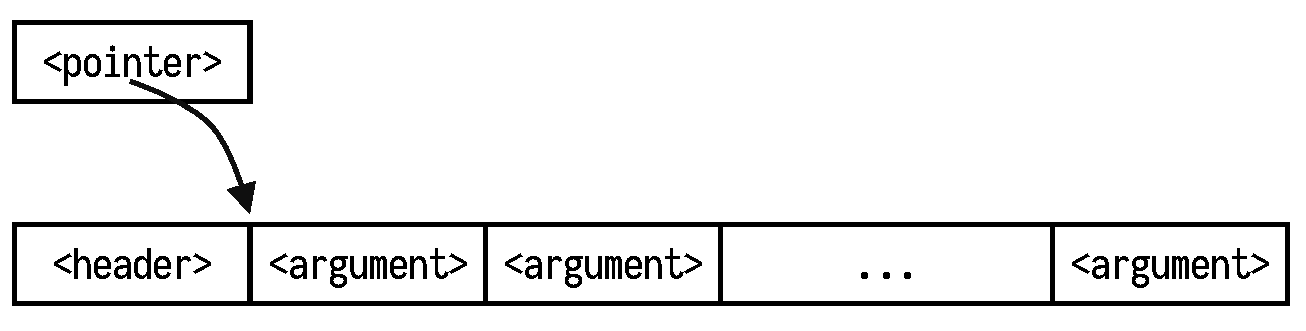
\includegraphics[scale=.59]{figures/boxed-value.pdf}
\centering
\caption{A \gls{boxed} representation of a \constructor{}.}
\end{figure}

\newpage
A \gls{boxed} value has a pointer address, which points to the second word of a block in memory where there is a \header{} and the arguments of the \constructor. 

Here is what the \header{} for a \gls{boxed} \constructor{} looks like when the word size is 64:

\begin{figure}[H]
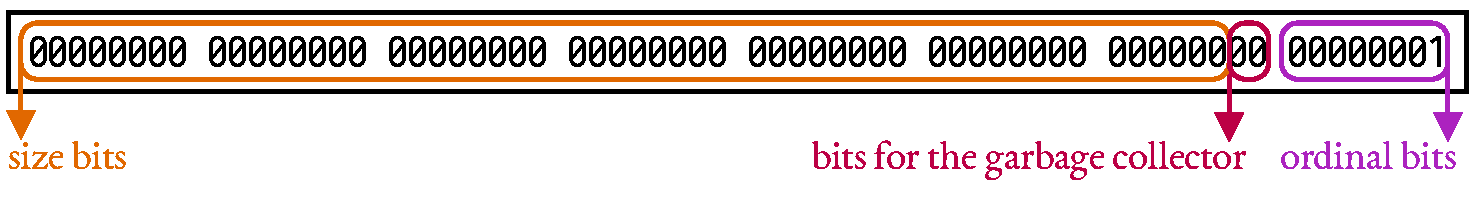
\includegraphics[scale=.59]{figures/boxed-header.pdf}
\centering
\caption{The header of a \gls{boxed} \constructor{}.}
\end{figure}

The first 22 or 54 bits (depending on the word size of the machine) of the \header{} signify the size of the block (in words) that comes after the \header{}. For a \gls{boxed} inductive Coq \constructor, this essentially means the number of arguments.\footnote{For types that have \glspl{parameter} or \glslink{index}{indices}, keep in mind that the parameter will not exist in runtime, but the index always will.}

Constructors that take no arguments have \gls{unboxed} representation, so there is no header, and no block, and no pointer: instead there is an odd number.

Here is what an unboxed constructor looks like when the word size is 64:

\begin{figure}[H]
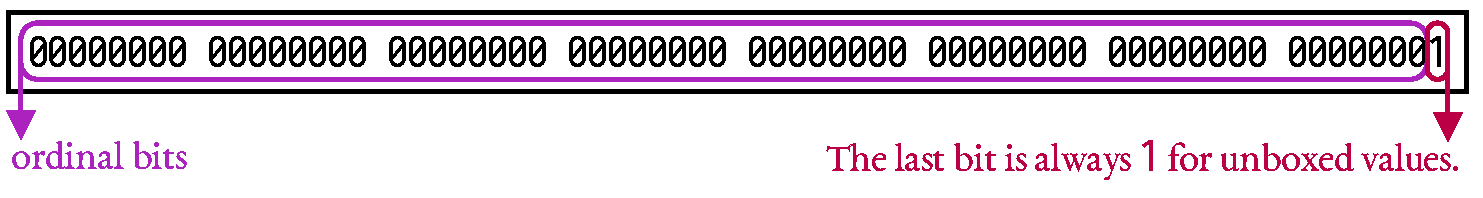
\includegraphics[scale=.59]{figures/unboxed-value.pdf}
\centering
\caption{An \gls{unboxed} representation of a \constructor{}.}
\end{figure}

Function \gls{closure}s are represented as a pointer to a block of memory, where a function pointer and its environment live. The environment is represented as a linked list in runtime. However, the environment is not typeable in Coq, as the values in the environments can be of different types.
% \todo{Higher-order, GraphPredicate of functions? call?}

\Gls{primitive} values have their own custom representations, which we will examine later in this thesis.

\subsection{Representation in the Heap Graph}

Based on the description above of CertiCoq's memory representation of values, one might assume that each Coq value has its own memory block. From a graph theory perspective, this assumption would have made the CertiCoq heap an \emph{out-forest}. Each Coq value would then be represented in the graph as an \emph{out-tree}. This, while elegant, is unfortunately not the case. DAGs in the heap graph can occur naturally: For terms such as \code{(\bn{x}, \bn{x})} or \code{[\bn{x}; \bn{x}; \bn{x}]}, the created object would be a DAG, not an out-tree. Even for Coq values that are created as out-trees initially, garbage collection can change the graph in a way that violates the tree properties, specifically because a path in the graph would not be necessarily unique anymore. The graph we arrive at is a \emph{directed acyclic graph} (DAG) but not an out-forest. The heap graph below is an example of this change: The object on the left can turn into the object on the right when the garbage collector runs, if we are using a hash-consing garbage collector~\cite{appel1993hash}.

\begin{figure}[H]
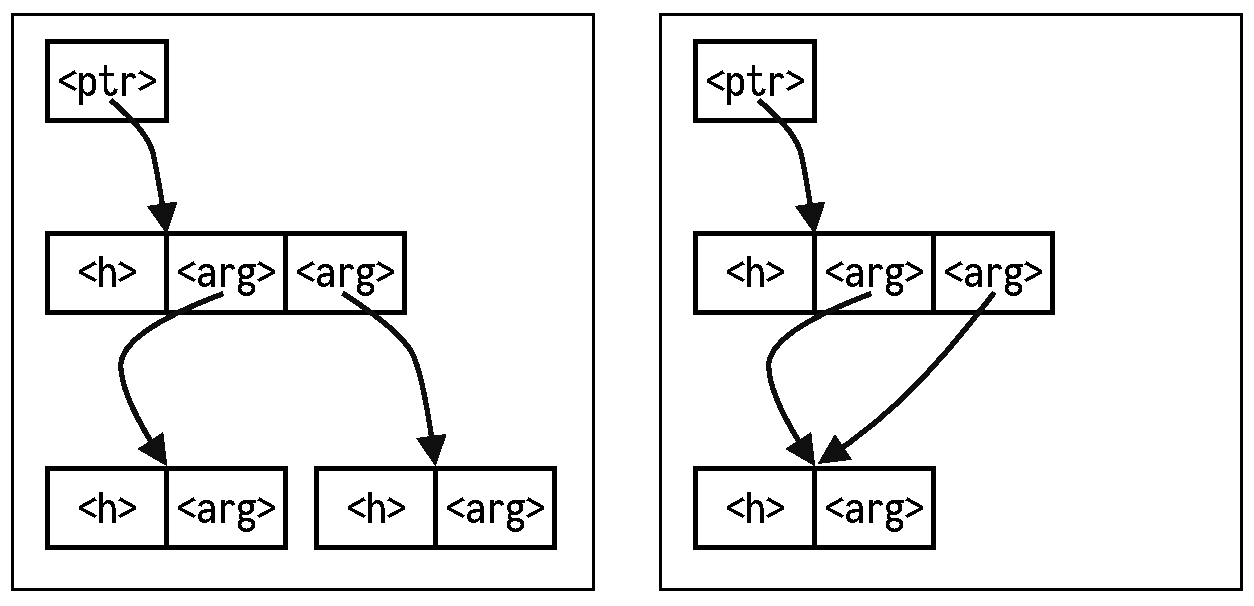
\includegraphics[scale=.49]{figures/gcdual.pdf}
\centering
\caption{Two possible memory representations of the term \code{(\dt{S O}, \dt{S O})}.}
\end{figure}

% Andrew's note:
% This is technically correct, but it is not the main reason that out-DAGs exist.   Most garbage collectors, including CertiCoq's current one, do not turn trees into DAGs.  Only the weird ones described in [Appel and Goncalves] would do that. Instead, the out-DAGs arise from ordinary interpreted or compiled Coq code, in which we can write (x,x) which creates a tuple that's already a DAG. (Or: x::x::x::nil)
% Hash-Consing Garbage Collection, by Andrew W. Appel and Marcelo J.R. Goncalves, Technical report TR-412-93, Department of Computer Science, Princeton University, January 1993.

Here on both sides, we see the term \code{(\dt{S O}, \dt{S O})}. The root of the \gls{boxed} \constructor{} for pairs. Each field of the pair is a boxed constructor for the successor constructor \dt{S}. In both of the successors, we see an \gls{unboxed} constructor \dt{O}. However, since the \dt{S O} value occurs twice, the garbage collector can free the memory used for one of them and have both values point to the same memory block so that the representation is shared between two values.

Since memory blocks are shared for different values, we cannot simply depend on the $\mathrel{*}$ connective in separation logic. At this point, we rely on previous work and use the CertiGraph library, which helps us reason about graph manipulating programs in VST~\cite{wang2019graph, shengyi2020mechanized}. The CertiGraph project developed a mechanically verified garbage collector for the CertiCoq runtime. We use both their garbage collector implementation in the CertiCoq runtime and their library of proofs to write our proofs about foreign functions.

\section{Definition of Representation Predicates}
\label{predicatedefns}

Correctness specifications of \constructor{} \glue{} functions and \gls{foreign function}s will involve (among other things) the correct interpretation and production of Coq values in the uniform representation we described above.
In this chapter, I will describe \emph{representation predicate}s, a mechanism to assert that a Coq value in CertiCoq's heap memory respects this uniform representation, and is equal to a certain Coq value. Using representation predicates, we can express specifications about the correctness and type safety of \glue{} functions and \gls{foreign function}s.


The memory representation of values is uniform, but only for values of \gls{inductive type}s and \gls{closure}s. \Gls{primitive} values and values of \gls{foreign type}s are allowed to have custom representations, therefore our system should be able to express custom representations. Therefore, we use Coq's type classes~\cite{sozeau2008first} to define graph predicates; this allows us to overload a single function name with different definitions for uniform representations of different \gls{inductive type}s, and also custom representations of \gls{foreign type}s:

\newcommand{\GraphPredicate}{\hyperref[code:GraphPredicate]{\ty{GraphPredicate}}}
\newcommand{\graphpredicate}{\hyperref[code:graphpredicate]{\fn{graph\_\linebreak[0]predicate}}}
\begin{Verbatim}
\kw{Class} \label{code:GraphPredicate}\GraphPredicate (\bn{A} : \ty{Type}) : \ty{Type} :=
  \{ \label{code:graphpredicate}\graphpredicate : \ty{graph} -> \ty{outlier_t} -> \bn{A} -> \ty{rep_type} -> \ty{Prop} \}.
\end{Verbatim}


We define a graph predicate as a function that takes the heap graph, the outliers (i.e.\ the values that are used but live outside of the \gls{CertiCoq heap}), an actual Coq value, and a heap representation, and produces a \ty{Prop} that posits that the heap representation represents the given Coq value in the heap graph properly.

For most types, we generate and use the common instance that follows the uniform representation. However, the type class mechanism allows the user to write custom instances of the \GraphPredicate{} type class, where the user can specify the layout of values of a particular type in the heap graph. As examples for custom representations, we will implement our own \gls{primitive} integers in \autoref{integers}, and our own \gls{primitive} strings in \autoref{bytestrings}.

During our proofs, we will need some lemmas about our graph predicate function. These lemmas are automatically proven for the uniform representation of inductive types, while the user will have to prove them by hand for custom representations. Because of the intricacy of their generation (explained further in \autoref{predicategen}), these lemmas live in a separate type class:

\newcommand{\InGraph}{\hyperref[code:InGraph]{\ty{InGraph}}}
\newcommand{\ingraphpred}{\hyperref[code:ingraphpred]{\fn{in\_\linebreak[0]graph\_\linebreak[0]pred}}}
\newcommand{\hasv}{\hyperref[code:hasv]{\fn{has\_v}}}
\newcommand{\ismonotone}{\hyperref[code:ismonotone]{\fn{is\_\linebreak[0]monotone}}}
\newcommand{\outliercompat}{\hyperref[code:outliercompat]{\fn{outlier\_\linebreak[0]compat}}}
\label{code:InGraph}
\label{code:ingraphpred}
\label{code:ismonotone}
\label{code:outliercompat}
\begin{Verbatim}
\kw{Class} \InGraph (\bn{A} : \ty{Type}) : \ty{Type} :=
  \{ \ingraphpred{} : \GraphPredicate \bn{A}
  ; \label{code:hasv}\hasv :
      \kw{forall} (\bn{g} : \ty{graph}) (\bn{outliers} : \ty{outlier_t}) (\bn{n} : \bn{A}) (\bn{v} : \ty{VType}),
        \graphpredicate \bn{g} \bn{outliers} \bn{n} (\fn{repNode} \bn{v}) -> \fn{graph_has_v} \bn{g} \bn{v}
  ; \ismonotone{} :
      \kw{forall} (\bn{g} : \ty{graph}) (\bn{outliers} : \ty{outlier_t}) (\bn{to} : \ty{nat}) (\bn{lb} : \ty{raw_vertex_block})
             (\bn{e} : \ty{list edge}) (\bn{n} : \bn{A}) (\bn{p} : \ty{rep_type}),
        \fn{add_node_compatible} \bn{g} (\fn{new_copied_v} \bn{g} \bn{to}) \bn{e} ->
        \fn{graph_has_gen} \bn{g} \bn{to} -> 
        \graphpredicate \bn{g} \bn{outliers} \bn{n} \bn{p} -> 
        \graphpredicate (\fn{add_node} \bn{g} \bn{to} \bn{lb} \bn{e}) \bn{outliers} \bn{n} \bn{p}
  ; \outliercompat{} : 
      \kw{forall} (\bn{g} : \ty{graph}) (\bn{outliers} : \ty{outlier_t}) (\bn{x} : \bn{A}) (\bn{p} : \ty{GC_Pointer}),
        \fn{outlier_compatible} \bn{g} \bn{outliers} ->
        \graphpredicate{} \bn{g} \bn{outliers} \bn{x} (\dt{repOut} \bn{p}) ->
        \ty{In} \bn{p} \bn{outliers}
  \}.
\end{Verbatim}

This type class contains
\begin{itemize}
\item the \GraphPredicate{} instance,
\item the \hasv{} lemma, which states that if a value is represented in the graph as a node, then the vertex of the node is in the graph,
\item the \ismonotone{} lemma, which states that a Coq value that is represented in memory properly can still be represented in memory if a new compatible node is added to the heap graph,
\item and the \outliercompat{} lemma, which states that if a Coq value is represented in the \gls{C heap} (as an \emph{outlier}), then that pointer will be in the outlier set.
\end{itemize}
The components of this type class are the work of Stark and Appel. This thesis does not require a deep understanding of these components because this thesis is mostly about writing foreign functions and their specifications, and not so much the proofs of these specifications. Therefore we will not go further in detail here, but the details of these lemmas can lemmas can be found in the tech report by Korkut, Stark, and Appel~\cite{korkutStarkAppel}.

Since we now have a type class hierarchy of \GraphPredicate{} and \InGraph{}, we also define the following helper function that projects the \graphpredicate{} field of the superclass \GraphPredicate{}, from an instance of the subclass \InGraph{}:

\newcommand{\isingraph}{\hyperref[code:isingraph]{\fn{is\_\linebreak[0]in\_\linebreak[0]graph}}}
\label{code:isingraph}
\begin{Verbatim}
\kw{Definition} \isingraph{} \{\bn{A} : \ty{Type}\} `\{\InGraph \bn{A}\}
                       : \ty{graph} -> \ty{outlier_t} -> \bn{A} -> \ty{rep_type} -> \ty{Prop} :=
  @\graphpredicate \bn{A} \ingraphpred.
\end{Verbatim}


Using these predicates, the users are empowered to write their own specifications and proofs for their foreign C functions. These predicates are also used to generate specifications and proofs for CertiCoq-generated glue functions, which can be used as building blocks for the foreign C functions and their correctness proofs.

For example, the \GraphPredicate{} instance for the \Vec{} inductive type looks like this:

% \newpage
\label{code:GraphPredicatevec}
\newcommand{\GraphPredicatevec}{\hyperref[code:GraphPredicatevec]{\fn{GraphPredicate\_\linebreak[0]vec}}}
\begin{Verbatim}
\kw{Instance} \GraphPredicatevec
         (\bn{A} : \ty{Type}) 
         (\bn{GraphPredicate_A} : \GraphPredicate{} \bn{A})
         (\bn{n} : \ty{nat}) : \GraphPredicate{} (\ty{vec} \bn{A} \bn{n}) :=
  \kw{let} \kw{fix} \fn{graph_predicate_vec} 
          (\bn{n} : \ty{nat})
          (\bn{g} : \ty{graph}) (\bn{outliers} : \ty{outlier_t}) (\bn{x} : \ty{vec} \bn{A} \bn{n}) (\bn{p} : \ty{rep_type})
          \{\kw{struct} \bn{x}\} : \ty{Prop} :=
    \kw{match} \bn{x} \kw{with}
    | \dt{vnil} => \fn{graph_cRep} \bn{g} \bn{p} (\dt{enum} \dt{0}) \dt{[]}
    | \dt{vcons} \bn{arg0} \bn{arg1} \bn{arg2} =>
        \kw{exists} \bn{p0} \bn{p1} \bn{p2} : \ty{rep_type},
          @\graphpredicate{} \ty{nat} \fn{GraphPredicate_nat} \bn{g} \bn{outliers} \bn{arg0} \bn{p0} \ty{/\textbackslash}
          @\graphpredicate{} \bn{A} \bn{GraphPredicate_A} \bn{g} \bn{outliers} \bn{arg1} \bn{p1} \ty{/\textbackslash}
          \fn{graph_predicate_vec} \bn{arg0} \bn{g} \bn{outliers} \bn{arg2} \bn{p2} \ty{/\textbackslash}
          \fn{graph_cRep} \bn{g} \bn{p} (\dt{boxed} \dt{0} \dt{3}) \dt{[}\bn{p0}\dt{;} \bn{p1}\dt{;} \bn{p2}\dt{]}
    \kw{end}
  \kw{in} \{| \graphpredicate{} := (\fn{graph_predicate_vec} \bn{n}) |\}.
\end{Verbatim}


\section{Generation of Representation Predicates}
\label{predicategen}

We generate for the \GraphPredicate{} and the \InGraph{} type classes using MetaCoq.

The \GraphPredicate{} type class only contains one field, the predicate function, and is generated entirely with MetaCoq. We made this design choice because the generated term has many moving parts: The instance has to quantify over the \gls{parameter}s and \indices{} of the inductive type. If those parameters are types, then the instance has to quantify over the \GraphPredicate{} instance of them. Parameters stay the same for the types in the same mutually inductive block, while indices can vary, which means the \kw{fix} we generate has to quantify over the indices. The \GraphPredicatevec{} example above demonstrates all of these moving parts.

Instances of the \InGraph{} type class, on the other hand, are generated using a combination of MetaCoq and \gls{Ltac}. We use MetaCoq only for generating the types of the instances and invoking \gls{Ltac} using \tmLemma{}. While these instances still have quantified \gls{parameter}s and \indices{}, the definitions inside an \InGraph{} instance do not need to use a \kw{fix} expression, so they are easier to discharge with \gls{Ltac} than to build with MetaCoq.

In this section, we will examine the problems we encounter with generating instances for the \GraphPredicate{} and \InGraph{} type classes, and present techniques to solve these problems.

\subsection{De Bruijn Notation Conversion}
\label{debruijnconversion}

In MetaCoq, variables are represented using a \emph{\gls{locally nameless}}~\cite{aydemir2008} approach\footnote{There is one caveat: While it is common to remove names from quantifiers in a \gls{locally nameless} representation, MetaCoq retains them.}. This means that free variables are represented as names, while bound variables are represented as de Bruijn indices~\cite{de1972lambda}. The \ty{term} type in MetaCoq, which deeply embeds the core terms of \gls{Gallina}, includes 4 constructors that are relevant to variables.

\begin{Verbatim}
\kw{Inductive} \ty{term} : \ty{Type} :=
    \dt{tRel} : \ty{nat} -> \ty{term}
  | \dt{tVar} : \ty{ident} -> \ty{term}
  | \dt{tEvar} : \ty{nat} -> \ty{list term} -> \ty{term}
  | \dt{tConst} : \ty{kername} -> \ty{Instance.t} -> \ty{term}
  ...
\end{Verbatim}

\dt{tRel} represents variables referred to by a de Bruijn index, where the lowest number in \dt{tRel} refers to the latest variable binding.
\dt{tVar} represents named variables introduced in Coq sections or interactive proofs~\cite{sozeau2020metacoq}. However, we will use \dt{tVar} for more than that soon.
\dt{tEvar} represents existential variables, which do not have locally nameless representation except in their sub\ty{term}s.
\dt{tConst} represents constants (but not inductive types or constructors), i.e. free variables that have a fully qualified name.

Let us consider an example of a quoted term that can help illustrate:

\vspace{.2in}
\begin{SaveVerbatim}{E}
\kw{MetaCoq Run} (\fn{tmQuote} (\kw{fun} (\bn{A} : \ty{Type}) (\bn{a} : \bn{A}) => \bn{a}) \fn{>>}\fn{=} \fn{tmPrint}).
\end{SaveVerbatim}
\tocoq{\UseVerbatim{E}}

\begin{SaveVerbatim}{E}
\dt{tLambda} \{| \fn{binder_name} := \dt{nNamed "A"}; \fn{binder_relevance} := \dt{Relevant} |\}
   (\dt{tSort} ...)
   (\dt{tLambda} \{| \fn{binder_name} := \dt{nNamed "a"}; \fn{binder_relevance} := \dt{Relevant} |\}
            (\dt{tRel 0})
            (\dt{tRel 0}))
\end{SaveVerbatim}
\fromcoq{\UseVerbatim{E}}

Here we are quoting the polymorphic identity function, which takes one argument \bn{A} that is a type, and one more argument \bn{a} of the type \bn{A}. However, notice that in the result of the quotation, the lambda body does not mention the type \bn{A} by name; it is represented by a de Bruijn index, represented by \dt{tRel 0}. This is observable in the second argument of the inner \dt{tLambda}.
The third argument of the inner \dt{tLambda} construction represents the function body in the original lambda, also happens to be \dt{tRel 0}. The new zeroth de Bruijn index refers to the argument \bn{a}, since the latest quantifier is \bn{a} now.

As we can see from this term, having quoted terms in de Bruijn notation can be confusing when inspecting quoted terms; it is even more confusing and error-prone to generate terms to unquote. This is because the code we want to generate will often have to deal with varying numbers of \indices{} or \gls{parameter}s of \gls{inductive type}s. Committing to generating code in de Bruijn notation will mean we have to keep track of how many of these \indices{} and \gls{parameter}s we have at a given time. Considering the possibility of our generated code introducing new quantifiers and having complicated dependent types that themselves can contain de Bruijn indices, it becomes clear that this is unsustainable.

Our solution is to misuse the \dt{tVar} constructor creatively to have a named representation for our terms. In this representation, all bound variables will be represented as \dt{tVar}s instead of \dt{tRel}s. We can define a function that converts between named and locally nameless representations. Any \ty{term} we receive from \TemplateMonad{} \gls{primitive}s or we pass into \TemplateMonad{} \gls{primitive}s will have locally nameless representation. But for the remaining internal computation, we can use our named representation.

\begin{Verbatim}
\kw{Definition} \ty{named_term} : \ty{Type} := \ty{term}.

\kw{Definition} \fn{deBruijn} (\bn{ctx} : \ty{list name}) (\bn{t} : \ty{named_term}) : \TemplateMonad{} \ty{term} :=
  ...
\kw{Definition} \fn{closed_deBruijn} (\bn{t} : \ty{named_term}) : \TemplateMonad{} \ty{term} :=
  \fn{deBruijn} \dt{nil} \bn{t}.

\kw{Definition} \fn{undeBruijn} (\bn{ctx} : \ty{list name})  (\bn{t} : \ty{term}) : \TemplateMonad{} \ty{named_term} :=
  ...
\kw{Definition} \fn{closed_undeBruijn} (\bn{t} : \ty{term}) : \TemplateMonad{} \ty{named_term} :=
  \fn{undeBruijn} \dt{nil} \bn{t}.
\end{Verbatim}

The \fn{deBruijn} and \fn{undeBruijn} implementations are quite straightforward. They adhere to the de Bruijn notation conversion definitions commonly found in programming language textbooks. We only needed to consider the dependent type system of the \gls{Gallina} core language and the fact that pattern matching in \kw{match} expressions can alter the number of bindings in the branch body.

\subsection{Type Class Resolution}

MetaCoq does not provide a mechanism for type class resolution under a context. We need to find a way to make unquotable \ty{term}s quotable (as we will explain) in order to use the \gls{primitive} resolution mechanism. Our solution for this problem is lambda lifting~\cite{johnsson1985lambda}. 

As seen in the \GraphPredicatevec{} instance above, we need to call \graphpredicate{} for the argument types of constructors. Given that \graphpredicate{} is a method of the \GraphPredicate{} type class, we have to make sure MetaCoq can figure out the type class instance to be used in the call. The initial solution most MetaCoq users would go for is to leave the instance argument as a \fn{hole}, and for MetaCoq to figure out how to fill the \fn{hole} during \gls{unquotation}. Unfortunately, this solution is currently not reliable enough, therefore we will have to infer these type class instances manually. MetaCoq only provides the following mechanism for type class resolution:

\vspace{.2in}
\begin{SaveVerbatim}{E}
\kw{Check} \fn{tmInferInstance}.
\end{SaveVerbatim}
\tocoq{\UseVerbatim{E}}

\begin{SaveVerbatim}{E}
\fn{tmInferInstance}
     : \ty{option reductionStrategy} -> 
       \kw{forall} \bn{A} : \ty{Type}, \TemplateMonad{} (\ty{option_instance} \bn{A})
\end{SaveVerbatim}
\fromcoq{\UseVerbatim{E}}

\newpage
Observe that this \TemplateMonad{} \gls{primitive} takes a \ty{Type}, and not a \ty{term}. This is easy to call with an actual type class constraint:

\vspace{.2in}
\begin{SaveVerbatim}{E}
\kw{MetaCoq Run} (\fn{tmInferInstance} (\dt{Some all}) 
                             (\kw{forall} \bn{A} `\{\ty{GraphPredicate} \bn{A}\} \bn{n},
                              \ty{GraphPredicate} (\ty{vec} \bn{A} \bn{n}))
             \fn{>>}\fn{=} \fn{tmPrint}).
\end{SaveVerbatim}
\tocoq{\UseVerbatim{E}}

\begin{SaveVerbatim}{E}
(\dt{my_Some} _ \fn{GraphPredicate_vec})
\end{SaveVerbatim}
\fromcoq{\UseVerbatim{E}}

However, when we inspect an \gls{inductive type}, we usually work with the reified versions of types and constructors. In order to use the \fn{tmInferInstance} \gls{primitive}, we would have to \unquote{} the \ty{term} into the Coq value it represents. Unfortunately, \unquoting{} can sometimes fail. Many intermediate forms we obtain while we compute results with \ty{term}s are not suitable to \unquoting{}. Consider the following function, one we actually use in the generation of \GraphPredicate{} instances:

\begin{Verbatim}
\kw{Fixpoint} \fn{strip_pis} (\bn{t} : \ty{named_term}) : \ty{named_term} :=
  \kw{match} \bn{t} \kw{with}
  | \dt{tProd} _ _ \bn{rest} => \fn{strip_pis} \bn{rest}
  | \bn{x} => \bn{x}
  \kw{end}.
\end{Verbatim}

This function takes a full function or constructor type, and removes the surrounding function type binders ($\Pi$-types, hence the function name). If it is given a term representing \code{\kw{forall} (\bn{A} : \ty{Type}), \bn{A}}, it will return a term that represents \bn{A}, i.e. the result type of the original function type.

This function generates unquotable terms for two reasons. One reason is that the stripped result type will contain free variables, therefore \unquoting{} will fail. The other reason is that this function generates \ty{named\_term}s, where we have a named representation instead of a de Bruijn notation, as described in \autoref{debruijnconversion}.
The former problem is handled by lambda lifting~\cite{johnsson1985lambda}, and the latter problem is handled by de Bruijn notation conversion. 

When we are generating the branches of the \kw{match} expression, we want to be able to call \graphpredicate{} on the arguments of constructors. However, we have to keep in mind that we are dealing with reified terms representing dependently typed arguments, in named representation. We will not be able to ask MetaCoq for an instance of \code{\GraphPredicate{} (\Vec{} \bn{A} \bn{n})} because since \bn{A} and \bn{n} are free variables, this type class is not even unquotable. To make it quotable, we have to turn it into a closed term by quantifying over the free variables, which we keep as the context, and convert it to de Bruijn notation. Then we can call the \fn{tmInferInstance} \gls{primitive}, as seen in the interaction above, and obtain the relevant \GraphPredicate{} instance. However, the call to \graphpredicate{} cannot solely pass \GraphPredicatevec{} as the instance, since the instance quantifies over the free variables even though the \graphpredicate{} call does not. Therefore we have apply the context to the instance object:

\vspace{.2in}
\begin{SaveVerbatim}{E}
\kw{Variable} (\bn{A} : \ty{Type})
         (\bn{GraphPredicate_A} : \GraphPredicate{} \bn{A})
         (\bn{n} : \ty{nat}).
\kw{Check} @\graphpredicate{} (\Vec{} \bn{A} \bn{n}) (\fn{GraphPredicate_vec} \bn{A} \bn{GraphPredicate_A} \bn{n}).
\end{SaveVerbatim}
\tocoq{\UseVerbatim{E}}

\begin{SaveVerbatim}{E}
\graphpredicate{}
     : \ty{graph} -> \ty{outlier_t} -> \ty{vec} \bn{A} \bn{n} -> \ty{rep_type} -> \ty{Prop}
\end{SaveVerbatim}
\fromcoq{\UseVerbatim{E}}

As seen in the arguments passed to \GraphPredicatevec{} here, applying the context makes the instance object type check.

\newpage
\subsection{Mutually Recursive Type Class Instances}

Coq allows definitions of mutually inductive data types:

\begin{Verbatim}
\kw{Inductive} \ty{tree} (\bn{A} : \ty{Type}) : \ty{Type} :=
| \dt{tleaf} : \ty{tree} \bn{A}
| \dt{tnode} : \bn{A} -> \ty{forest} \bn{A} -> \ty{tree} \bn{A}
\kw{with} \ty{forest} (\bn{A} : \ty{Type}) : \ty{Type} :=
| \dt{fnil} : \ty{forest} \bn{A}
| \dt{fcons} : \ty{tree} \bn{A} -> \ty{forest} \bn{A} -> \ty{forest} \bn{A}.
\end{Verbatim}

Coq allows definitions of mutually recursive functions as well:

\begin{Verbatim}
\kw{Fixpoint} \fn{tree_size} \{\bn{A} : \ty{Type}\} (\bn{t} : \ty{tree} \bn{A}) : \ty{nat} :=
  \kw{match} \bn{t} \bn{with}
  | \dt{tleaf} => \dt{0}
  | \dt{tnode} _ \bn{f} => \dt{1} \fn{+} \fn{forest_size} \bn{f}
  \kw{end}
\kw{with} \fn{forest_size} \{\bn{A} : \ty{Type}\} (\bn{f} : \ty{forest} \bn{A}) : \ty{nat} :=
  \kw{match} \bn{f} \kw{with}
  | \dt{fnil} => \dt{0}
  | \dt{fcons} \bn{t} \bn{f} => \fn{tree_size} \bn{t} + \fn{forest_size} \bn{f}
  \kw{end}.
\end{Verbatim}

Notice that \kw{Fixpoint} is a vernacular command that can create multiple, mutually recursive definitions. 

However, MetaCoq does not provide a \TemplateMonad{} \gls{primitive} to create multiple definitions together. It only allows making a \gls{Gallina} term into a single definition. In \gls{Gallina} you cannot define both definitions at once, you have to define each function separately. \gls{Gallina}'s syntax for mutually recursive functions allows locally defining all functions but then exporting a single one of them at the end (with \kw{for} followed by an identifier). Here is what these two functions would look like as stand-alone definitions:

\begin{Verbatim}
\kw{Definition} \fn{tree_size} :=
  \kw{fix} \fn{tree_size} \{\bn{A} : \ty{Type}\} (\bn{t} : \ty{tree} \bn{A}) : \ty{nat} :=
    \kw{match} \bn{t} \bn{with}
    | \dt{tleaf} => \dt{0}
    | \dt{tnode} _ \bn{f} => \dt{1} \fn{+} \fn{forest_size} \bn{f}
    \kw{end}
  \kw{with} \fn{forest_size} \{\bn{A} : \ty{Type}\} (\bn{f} : \ty{forest} \bn{A}) : \ty{nat} :=
    \kw{match} \bn{f} \kw{with}
    | \dt{fnil} => \dt{0}
    | \dt{fcons} \bn{t} \bn{f} => \fn{tree_size} \bn{t} + \fn{forest_size} \bn{f}
    \kw{end}.
  \kw{for} \fn{tree_size}.

\kw{Fixpoint} \fn{forest_size} \{\bn{A} : \ty{Type}\} (\bn{f} : \ty{forest} \bn{A}) : \ty{nat} :=
  \kw{match} \bn{f} \kw{with}
  | \dt{fnil} => \dt{0}
  | \dt{fcons} \bn{t} \bn{f} => \fn{tree_size} \bn{t} + \fn{forest_size} \bn{f}
  \kw{end}.
\end{Verbatim}

Notice that we had to repeat the body of the \fn{forest\_size} function. Given that it is a separate definition, any theorems we prove about the outer \fn{forest\_size} do not directly apply to the inner \fn{forest\_size}; we would have to unfold the definition to make sure that they are the same underneath.

Now, given these restrictions, let us reimagine type class instance generation for mutually inductive types.

When we define a \GraphPredicate{} instance for a type in a mutually inductive type block, we want to check if we already have \GraphPredicate{} instances for the other types in the block. If there are, then we do not have to generate \graphpredicate{} functions in a \kw{fix} block for them; we can simply call the existing instances if there are mutually recursive calls. If there are no instances for the types in the same mutually inductive block, then we generate all \graphpredicate{} functions for the types in that block, place them in a \kw{fix} expression, and return only one of them. For example, the generated \GraphPredicate{} instance for the \ty{tree} type above would look like this:

\label{code:GraphPredicatetree}
\newcommand{\GraphPredicatetree}{\hyperref[code:GraphPredicatetree]{\fn{GraphPredicate\_\linebreak[0]tree}}}
\newcommand{\graphpredicatetree}{\hyperref[code:GraphPredicatetree]{\fn{graph\_\linebreak[0]predicate\_\linebreak[0]tree}}}
\newcommand{\graphpredicateforest}{\hyperref[code:GraphPredicatetree]{\fn{graph\_\linebreak[0]predicate\_\linebreak[0]forest}}}
\begin{Verbatim}
\kw{Instance} \GraphPredicatetree
         (\bn{A} : \ty{Type})
         (\bn{GraphPredicate_A} : \ty{GraphPredicate} \bn{A}) : \ty{GraphPredicate} (\ty{tree} \bn{A}) :=
  \kw{let} \bn{f} :=
    \kw{fix} \graphpredicatetree
        (\bn{g} : \ty{graph}) (\bn{outliers} : \ty{outlier_t}) (\bn{x} : \ty{tree} \bn{A}) (\bn{p} : \ty{rep_type}) 
        \{\kw{struct} \bn{x}\} : \ty{Prop} :=
      \kw{match} \bn{x} \kw{with}
      | \dt{tleaf} => \fn{graph_cRep} \bn{g} \bn{p} (\dt{enum} \dt{0}) \dt{[]}
      | \dt{tnode} \bn{arg0} \bn{arg1} =>
          \kw{exists} \bn{p0} \bn{p1} : \ty{rep_type},
            @\graphpredicate{} \bn{A} \bn{GraphPredicate_A} \bn{g} \bn{outliers} \bn{arg0} \bn{p0} \ty{/\textbackslash}
            \graphpredicateforest{} \bn{g} \bn{outliers} \bn{arg1} \bn{p1} \ty{/\textbackslash}
            \fn{graph_cRep} \bn{g} \bn{p} (\dt{boxed} \dt{0} \dt{2}) \dt{[}\bn{p0}\dt{;} \bn{p1}\dt{]}
      \kw{end}
    \kw{with} \graphpredicateforest
         (\bn{g} : \ty{graph}) (\bn{outliers} : \ty{outlier_t}) (\bn{x} : \ty{forest} \bn{A}) (\bn{p} : \ty{rep_type})
         \{\kw{struct} \bn{x}\} : \ty{Prop} :=
      \kw{match} \bn{x} \kw{with}
      | \dt{fnil} => \fn{graph_cRep} \bn{g} \bn{p} (\dt{enum} \dt{0}) \dt{[]}
      | \dt{fcons} \bn{arg0} \bn{arg1} =>
          \kw{exists} \bn{p0} \bn{p1} : \ty{rep_type},
            \graphpredicatetree{} \bn{g} \bn{outliers} \bn{arg0} \bn{p0} \ty{/\textbackslash}
            \graphpredicateforest{} \bn{g} \bn{outliers} \bn{arg1} \bn{p1} \ty{/\textbackslash}
            \fn{graph_cRep} \bn{g} \bn{p} (\dt{boxed} \dt{0} \dt{2}) \dt{[}\bn{p0}\dt{;} \bn{p1}\dt{]}
      \kw{end}
    \kw{for} \graphpredicatetree
  \kw{in} \{| \graphpredicate{} := \bn{f} |\}.
\end{Verbatim}

If we want to generate a \GraphPredicate{} instance for the \ty{forest} type as well, that can now use the \GraphPredicatetree{} instance.

% The traditional way of defining mutually recursive functions is ..., but this is technically not a part of Gallina; it is a part of the vernacular language. % todo link vernacular

% Gallina does allow mutually recursive functions with the \kw{fix} syntax ...

% % the correct solution: fix returning a tuple of all the functions ?
% % no, this cannot use other instances

% Mutually recursive type class instance calls requires a two-pass mechanism for instance generation. In the first pass, we generate bogus names, globally unique identifiers, for the recursive calls. In the second pass, we substitute the bogus names with the actual calls.

\chapter{Reification with Annotations}
\label{reified}

\epigraph{
% Reflexivity is taken for granted, as the premise for a sign system such as natural languages.\\On the other hand, t
[T]he inherent risk of unintelligibility of reflexivity, has been noted\\ throughout human history in countless paradoxes. For example, in a Greek myth,\\Narcissus became immobile as a result of staring at his own reflection in the water.}{Kumiko Tanaka-Ishii~\cite{tanaka2010semiotics}}

Obtaining a specification from a \gls{foreign function}'s type or a \constructor{}'s type requires the ability to traverse the components of the type. Such a traversal requires a method to inspect types (or at least \constructor{}s' types) as first-class constructs. In this chapter, we will examine why the existing methods fall short of serving our purposes, and we will introduce a new method that solves our problem.

Traversing types is necessary in many different kinds of homogeneous code generation, therefore the generic programming and \gls{metaprogramming} literature has been preoccupied with it: The Generic Haskell literature achieved code generation at runtime through a representation of Haskell's algebraic data types by deconstructing them into a type that identifies its sums, products, and atomic components~\cite{jansson1997, hinze2003chapter}. The Template Haskell literature achieved code generation at compile time through a language \gls{primitive} that supplies information about algebraic data types~\cite{sheard2002template}.

MetaCoq follows the Template Haskell tradition. MetaCoq's \fn{tmQuoteRec} command in the \TemplateMonad{} provides all the information about any inductive type and its constructors. However, this data is not designed for quick and easy consumption, as it provides a \glslink{deep embedding}{deeply embedded} description of the types, where all the terms are represented in the core language and they are not easily reflectable. The use of \fn{tmQuoteRec} we have seen in \autoref{metacoq} epitomizes the difficulty of parsing through the output in order to generate code quickly.

There are two main challenges contributing to the difficulty: Firstly, the MetaCoq representation requires explicit handling of names in binders, even after converting to named representation. Secondly, the \ty{term}s obtained from MetaCoq cannot be reflected without their complete contexts. The solution we will present for our original problem of generating specifications for functions' and \constructor{}s' types, will have to address these challenges.

Handling names and binders has long been a persistent issue in programming languages. One popular solution that circumvents the issue is \emph{higher-order abstract syntax}~\cite{hoas}, which allows a language implementation to depend on the binding mechanism of the \gls{host language} to implement binding for an \gls{object language}. From a dependent types point of view, using the binders of the \gls{host language} allows proper typing of all dependently typed arguments. This convenience makes higher-order abstract syntax a good starting point for our solution.

However, our requirements in this thesis are different from describing terms in any language. Unlike higher-order abstract syntax, we do not need to describe a full language. We only need to describe functions' or \constructor{}s' types, where every component is a type. We need to be able to traverse the components of the type, and to consider how a given component should affect the specification for that \gls{foreign function} or \constructor{}. This requires us to consume a type and produce a specification. While dependent type systems allow us to take a type as an argument, Coq does not allow us to inspect types at runtime.\footnote{Unlike Idris 2, another dependently typed language, which has the \emph{type-case} feature that allows inspection of types at runtime.} Coq's mechanism that allows us to inspect types and obtain different values accordingly is type classes, which are resolved at compile time. Since we are not allowed to look for type class instances at runtime, we should find them at compile time and annotate our representation with the appropriate type class instances.

Following the fundamental theorem of computer science\footnote{``We can solve any problem by introducing an extra level of indirection'', attributed to David J. Wheeler.}, we introduce a new way to represent function types as data, an intermediate representation between MetaCoq and function specifications. We will use \gls{metaprogramming} to obtain MetaCoq's representation of inductive types and constructors to convert them into our representation, and then we can generate the specifications we need from our intermediate representation, in pure \gls{Gallina}. This isolates \gls{metaprogramming} to the first half of this conversion, and simplifies the specification generation later, and also allows us to reason about the specification generation if we ever decide to, though we leave that as future work.

At the heart of this intermediate representation is our description type, which is defined as such:

\newcommand{\reified}{\hyperref[code:reified]{\ty{reified}}}
\newcommand{\TYPEPARAM}{\hyperref[code:TYPEPARAM]{\dt{TYPEPARAM}}}
\newcommand{\ARG}{\hyperref[code:ARG]{\dt{ARG}}}
\newcommand{\RES}{\hyperref[code:RES]{\dt{RES}}}
\begin{Verbatim}
\kw{Inductive} \reified\label{code:reified} (\bn{ann} : \ty{Type} -> \ty{Type}) : \ty{Type} :=
| \TYPEPARAM\label{code:TYPEPARAM} : (\kw{forall} (\bn{A} : \ty{Type}) `\{\bn{ann} \bn{A}\}, \reified{} \bn{ann}) -> \reified{} \bn{ann}
| \ARG\label{code:ARG} : \kw{forall} (\bn{A} : \ty{Type}) `\{\bn{ann} \bn{A}\}, (\bn{A} -> \reified{} \bn{ann}) -> \reified{} \bn{ann}
| \RES\label{code:RES} : \kw{forall} (\bn{A} : \ty{Type}) `\{\bn{ann} \bn{A}\}, \reified{} \bn{ann}.
\end{Verbatim}

\begin{itemize}
\item The \TYPEPARAM{} constructor represents type parameters of a function or a \constructor{}. It takes a higher-order function as an argument, where the function takes a Coq type \bn{A} as an argument, along with a guarantee that there is an instance of the \bn{ann} type class, and returns another \reified{} description. This way the rest of the description has access to the type parameter and its type class instance in the context.

\item The \ARG{} constructor represents dependent arguments of a function or a \constructor{}.
\ARG{} takes the type of the argument, a witness that there is a type class instance for that type, and finally a higher-order function that takes an argument and returns a \reified{} description. This argument allows us to express dependently typed arguments, since the argument of the higher-order function can be occur in the rest of the description.

\item Finally, the \RES{} constructor represents the result type of a function. \RES{} takes the result type, and a witness that there is a type class instance for that type.
\end{itemize}

Our representation is a combination of \emph{\gls{deep embedding}} and \emph{\gls{shallow embedding}} techniques.
\glslink{deep embedding}{Deep embedding} is a syntactic description, where constructing an abstract syntax tree is the priority, while \gls{shallow embedding} is a representation where the terms are represented directly in their semantics~\cite{gibbons2014folding}. The description type that would solve our problems had to be traversable, therefore we defined it as an \gls{inductive type}, like a \gls{deep embedding}. In the arguments of each \constructor{}, however, we see the Coq semantics of the respective concept: for a type parameter, we have a function that takes a type parameter, for an argument we have a function that takes an argument, resembling a \gls{shallow embedding}. This approach allows us to closely resemble the original function or \constructor{}, while clearly identifying each part in the type.

Using the \reified{} type, we can now describe types of functions or \constructor{}s. While we use it for generating specifications, the \reified{} type is general-purpose in essence. The \gls{parameter} \bn{ann} allows descriptions to be annotated with instances of any type class that fits the type \code{\ty{Type} \code{-}\code{>} \ty{Type}}.

Before moving on to generating specifications from \reified{} descriptions, let us examine a simpler use of this type.
Let us define a type class that tells us how to convert values of a given data type into strings, similar to Haskell's \ty{Show} type class. We can define instances of this type class for some commonly used types, such as \ty{nat}, \ty{bool}, and \ty{list}.

% \kw{Instance} \fn{ToString_nat} : \ty{ToString} \ty{nat} :=
%   \{| \fn{to_string} (\bn{n} : \ty{nat}) := \fn{string_of_nat} \bn{n} |\}.
  
% \kw{Instance} \fn{ToString_bool} : \ty{ToString} \ty{bool} :=
%   \{| \fn{to_string} (\bn{b} : \ty{bool}) := \kw{if} \bn{b} \kw{then} \dt{"true"} \kw{else} \dt{"false"} |\}.
  
% \kw{Instance} \fn{ToString_list} \{\bn{A} : \ty{Type}\} `\{\ty{ToString} \bn{A}\} : \ty{ToString} (\ty{list} \bn{A}) :=
%   \{| \fn{to_string} := \kw{fix} \fn{f} (\bn{xs} : \ty{list} \bn{A}) : \ty{string} :=
%        \kw{match} \bn{xs} \kw{with}
%        | \dt{nil} => \dt{"nil"}
%        | \dt{cons} \bn{y} \bn{ys} => \fn{to_string} \bn{y} \fn{+}\fn{+} \dt{" :: "} \fn{+}\fn{+} \fn{f} \bn{ys}
%        \kw{end}
%    |\}.



\newcommand{\ToString}{\hyperref[code:ToString]{\ty{ToString}}}
\newcommand{\tostring}{\hyperref[code:tostring]{\fn{to\_\linebreak[0]string}}}

\begin{Verbatim}
\kw{Class} \ToString{}\label{code:ToString} (\bn{A} : \ty{Type}) := \{ \tostring{}\label{code:tostring} : \bn{A} -> \ty{string} \}.
\kw{Instance} \fn{ToString_nat} : \ToString{} \ty{nat} := \cm{...}
\kw{Instance} \fn{ToString_bool} : \ToString{} \ty{bool} := \cm{...}
\kw{Instance} \fn{ToString_list} \{\bn{A} : \ty{Type}\} `\{\ToString{} \bn{A}\} : \ToString{} (\ty{list} \bn{A}) := \cm{...}
\end{Verbatim}

Now, suppose we want to describe the type of this function:

\begin{Verbatim}
\fn{length} : \kw{forall} \{\bn{A} : \ty{Type}\}, \ty{list} \bn{A} -> \ty{nat}
\end{Verbatim}

The function type consists of a type parameter, an argument that follows it, and finally the result type. The \reified{} description of it also follows the same order:

\newcommand{\lengthdesc}{\hyperref[code:lengthdesc]{\fn{length\_\linebreak[0]desc}}}
\begin{Verbatim}
\kw{Definition} \lengthdesc{}\label{code:lengthdesc} : \reified{} \ToString{} :=
  \TYPEPARAM{} (\kw{fun} (\bn{A} : \ty{Type}) \{\bn{H_A} : \ToString{} \bn{A}\} =>
    \ARG{} (\ty{list} \bn{A}) (\kw{fun} (_ : \ty{list} \bn{A}) =>
      \RES{} \ty{nat})).
\end{Verbatim}

The annotation type we picked, namely \ToString{}, is visible in the type of \lengthdesc{}. In the definition, the \bn{H\_A} is visible, while the annotations in the \dt{ARG} and \dt{RES} constructors are implicit arguments, so they are hidden. Since the implicit arguments are type class instances, Coq's type class resolution system should be able to figure out the instance terms. However, we can choose to write the same description with explicit annotations:

\begin{Verbatim}
\kw{Definition} \lengthdesc{} : \reified{} \ToString{} :=
  @\TYPEPARAM{} _ (\kw{fun} (\bn{A} : \ty{Type}) \{\bn{H_A} : \ToString{} \bn{A}\} =>
    @\ARG{} _ (\ty{list} \bn{A}) (@\fn{ToString_list} \bn{A} \bn{H_A}) (\kw{fun} (_ : \ty{list} \bn{A}) =>
      @\RES{} _ \ty{nat} \fn{ToString_nat})).
\end{Verbatim}

\section{Consuming Reified Descriptions}

\newcommand{\args}{\hyperref[code:args]{\fn{args}}}
Now we have an example annotation, which makes it easier to demonstrate the functions that consume \reified{} descriptions. One of these functions is \args{}, which takes a \reified{} description and generates a nested dependent tuple of the types of all type parameters and arguments in the description:

\begin{Verbatim}
\kw{Fixpoint} \args{}\label{code:args} \{\bn{cls} : \ty{Type} -> \ty{Type}\} (\bn{c} : \reified{} \bn{cls}) : \ty{Type} :=
  \kw{match} \bn{c} \kw{with}
  | \TYPEPARAM{} \bn{k} => \{\bn{A} : \ty{Type} & \{\bn{H} : \bn{cls} \bn{A} & \args{} (\bn{k A H})\}\}
  | \ARG{} \bn{A H k} => \{\bn{a} : \bn{A} & \args{} (\bn{k a})\}
  | \RES{} _ _ => \ty{unit}
  \kw{end}.
\end{Verbatim}

The type parameter case adds two fields to the tuple, one for the type, and one for the type class instance. The type class instance has to be there so that we can later call the function \bn{k}, whose result we can use for a recursive call, which allows the traversal of the \reified{} description to continue. The argument case adds one field to the tuple, the argument. The result (\RES{}) case is the base case, it adds the \ty{unit} type as a stop to the nested tuple.

Notice that \args{} generates a \ty{Type} at the end, which means we can have terms that have the type \args{} of some description. For the description of the \fn{length} function we had above, this term would look as such:

\newcommand{\lengthargs}{\hyperref[code:lengthargs]{\fn{length\_\linebreak[0]args\_\linebreak[0]example}}}
\begin{Verbatim}
\kw{Definition} \lengthargs{}\label{code:lengthargs} : \args{} \lengthdesc{} :=
  (\ty{bool}; (\fn{ToString_bool}; ([\dt{true}; \dt{false}]; \dt{tt}))).
\end{Verbatim}

We should note that this term looks like an example call of the \fn{length} function, namely \code{@\fn{length} \ty{bool} [\dt{true}; \dt{false}]}, which should illustrate why we developed this mechanism: When we need to write a function that needs to quantify over all the arguments that a function or a \constructor{} takes, we can use \args{} of a \reified{} description to achieve that.

% One such function is one 
Let us write one such function. Since our description \lengthargs{} is annotated by the \ToString{} type class, we can design a function that would take the \args{} for a \fn{length} function as an argument, and build a \ty{string} that contains all the arguments converted to a \ty{string}. That function, generalized to any \reified{} description, would look like this:

\newcommand{\appenddescs}{\hyperref[code:appenddescs]{\fn{append\_\linebreak[0]descs}}}
% \begin{Verbatim}
% \kw{Fixpoint} \appenddescs{}\label{code:appenddescs} (\bn{r} : \reified{} \ToString{}) : \args{} \bn{r} -> \ty{string} :=
%   \kw{match} \bn{r} \kw{as} \bn{l} \kw{return} (\args{} \bn{l} -> \ty{string}) \kw{with}
%   | \TYPEPARAM{} \bn{k} =>
%       \kw{fun} '(\bn{A}; (\bn{H}; \bn{rest})) => \appenddescs{} (\bn{k} \bn{A} \bn{H}) \bn{rest}
%   | \ARG{} \bn{A} \bn{H} \bn{k} =>
%       \kw{fun} '(\bn{a}; \bn{rest}) => \tostring{} \bn{a} \fn{+}\fn{+} \dt{" | "} \fn{+}\fn{+} \appenddescs{} (\bn{k} \bn{a}) \bn{rest}
%   | \RES{} \bn{A} \bn{H} => \kw{fun} '\dt{tt} => \dt{""}
%   \kw{end}.
% \end{Verbatim}

\begin{Verbatim}
\kw{Equations} \appenddescs{}\label{code:appenddescs} (\bn{r} : \reified{} \ToString{}) (\bn{xs} : \args{} \bn{r}) : \ty{string} :=
\appenddescs{} (@\TYPEPARAM{} \bn{k}) (\bn{A}; (\bn{H}; \bn{rest})) :=
  \appenddescs{} (\bn{k} \bn{A} \bn{H}) \bn{rest} ;
\appenddescs{} (@\ARG \bn{A} \bn{H} \bn{k}) (\bn{a}; \bn{rest}) := 
  \tostring{} \bn{a} \fn{+}\fn{+} \dt{" | "} \fn{+}\fn{+} \appenddescs{} (\bn{k} \bn{a}) \bn{rest} ;
\appenddescs{} (@\RES{} _ _) \dt{tt} := \dt{""}.
\end{Verbatim}

This function uses dependent pattern matching, where the type of the second argument depends on the value of the first argument.
While it is possible to write functions with dependent pattern matching in pure \gls{Gallina}, we present these function definitions using the Equations plugin~\cite{sozeau2019equations} for easier understanding. We will continue this presentation in other consumers of \reified{} descriptions when necessary, to avoid convoluted \gls{Gallina} expressions.

We can observe the dependent pattern matching in how the type of the second argument changes: In the \TYPEPARAM{} case, the \args{} object, is a nested dependent pair of \bn{A}, the type, \bn{H\_A}, the \ToString{} instance, and \bn{rest}, the rest of the \args{} object.
In the \ARG{} case, the \args{} object is a dependent pair of \bn{a}, which is the argument of type \bn{A}, and \bn{rest}, the rest of the \args{} object.
In the \RES{} case, the \args{} function arrives at its base case, therefore the \args{} object is \dt{tt}, the constructor for the \ty{unit} type.
This is a pattern we should expect in functions that take an \args{} object as an argument.

Let us call the \appenddescs{} function with a \reified{} description and an \args{} object that fits that description, and observe the result we get:

\vspace{.2in}
\begin{SaveVerbatim}{E}
\kw{Compute} (\appenddescs{} \lengthdesc{} \lengthargs{}).
\end{SaveVerbatim}
\tocoq{\UseVerbatim{E}}

\begin{SaveVerbatim}{E}
  = \dt{"true :: false :: nil | "}
  : \ty{string}
\end{SaveVerbatim}
\fromcoq{\UseVerbatim{E}}


\newcommand{\result}{\hyperref[code:result]{\fn{result}}}

Now that we have seen how to write functions that consume \reified{} descriptions, such as \args{} and \appenddescs{}, we can write more functions like that. A remarkably useful one is \result{}, that traverses the \reified{} description of a function or \constructor{} type and returns the result type of that function:

% \begin{Verbatim}
% \kw{Fixpoint} \result{}\label{code:result} \{\bn{cls} : \ty{Type} -> \ty{Type}\}
%          (\bn{c} : \reified{} \bn{cls}) : \args{} \bn{c} -> \{\bn{A} : \ty{Type} & \bn{cls} \bn{A}\} :=
%   \kw{match} \bn{c} \kw{as} \bn{l} \kw{return} (\args{} \bn{l} -> \{\bn{A} : \ty{Type} & \bn{cls} \bn{A}\}) \kw{with}
%   | \TYPEPARAM{} \bn{k} => \kw{fun} '(\bn{A}; (\bn{H}; \bn{rest})) => \result{} (\bn{k} \bn{A} \bn{H}) \bn{rest}
%   | \ARG{} \bn{A} \bn{H} \bn{k} => \kw{fun} '(\bn{a}; \bn{rest}) => \result{} (\bn{k} \bn{a}) \bn{rest}
%   | \RES{} \bn{A} \bn{H} => \kw{fun} _ => (\bn{A}; \bn{H})
%   \kw{end}.
% \end{Verbatim}

\begin{Verbatim}
\kw{Equations} \result{}\label{code:result} (\bn{r} : \reified{} \ToString{}) (\bn{xs} : \args{} \bn{r}) : \ty{Type} :=
\result{} (@\TYPEPARAM{} \bn{k}) (\bn{A}; (\bn{H}; \bn{rest})) := \result{} (\bn{k} \bn{A} \bn{H}) \bn{rest} ;
\result{} (@\ARG \bn{A} \bn{H} \bn{k}) (\bn{a}; \bn{rest}) := \result{} (\bn{k} \bn{a}) \bn{rest};
\result{} (@\RES{} \bn{A} \bn{H}) \dt{tt} := (\bn{A}; \bn{H}).
\end{Verbatim}

We traverse the \reified{} description, by obtaining the rest of the description by calling \bn{k} and recursing. In \RES{}, our base case, we return the type that lives in the constructor field \bn{A}. This is a good example of how we reap the benefits of our representation, which is only a valid Coq term because of all the context we preserved in the higher-order abstract syntax.

Now, using \args{} and \result{}, we can write a function that gives us a type that is as close as possible to the original function or \constructor{} type. In other words, we want to \glslink{reflection}{reflect} the type description to an actual Coq type:

\newcommand{\reflect}{\hyperref[code:reflect]{\fn{reflect}}}
\begin{Verbatim}
\kw{Definition} \reflect{}\label{code:reflect} \{\bn{cls} : \ty{Type} -> \ty{Type}\} (\bn{r} : \reified{} \bn{cls}) : \ty{Type} :=
  \kw{forall} (\bn{P} : \args{} \bn{r}), \fn{projT1} (\result{} \bn{r} \bn{P}).
\end{Verbatim}

The type we obtain from this function is essentially the uncurried version of the type of \fn{length}. A function of type \code{\reflect{} \lengthdesc{}} would take a nested dependent tuple of all the arguments (and the annotations for type parameters) and return the same result type. Here is how that function would be implemented: 

\begin{Verbatim}
\kw{Definition} \fn{length_uncurried} : \reflect{} \lengthdesc{} :=
  \kw{fun} '(\bn{A}; (_; (\bn{l}; \dt{tt}))) => @\fn{length} \bn{A} \bn{l}.
\end{Verbatim}

The \reflect{} function provides a type-safe way for us to go from the description into the original function. Using \reflect{}, we can make sure that the function we have fits the description we were provided. 

While it was feasible to derive the curried function type, which closely resembles the original \constructor{} or \gls{foreign function} type, we deliberately opted for the uncurried function in our implementation of \reflect{}. This choice was driven by the necessity of uncurried functions in our function specifications outlined in \autoref{ctorspecs} and \autoref{primspecs}.~\footnote{VST's \kw{WITH} clauses have an easier time with a nested dependent tuple of arguments than many dependent arguments. Also, the language of our \gls{foreign function}, C, has naturally uncurried functions.} 
The other reason for this choice is that the uncurried function type includes the annotation arguments, while the curried function does not. Therefore producing the curried one from the uncurried one makes more sense than producing the uncurried one from the curried one, since we do not have to make up bogus annotations in the former. Although we avoided the latter approach in the general scenario, a specific use case taking this route (traversal of a \reified{} description without an \args{} object) is presented in \autoref{primspecs}.

% Another factor in this choice was that converting a curried function to its uncurried counterpart without resorting to \gls{metaprogramming} seemed less intuitive. Our uncurried representation retains annotation arguments in \args{}, for each \TYPEPARAM{}, whereas a curried representation would ideally omit them to precisely match the original \constructor{}'s type. This would entail defining an unnatural default \bn{ann} instance applicable to any type, which would be used when invoking the functions \bn{k} during traversal of the \reified{} descriptions. 

In \autoref{ctordesc} and \autoref{primdesc}, we explore detailed examples that showcase reified descriptions and their transformation into concrete Coq values. We leverage \reified{} descriptions of Coq \constructor{}s and custom \gls{primitive} functions to create VST specifications for the generated glue code and foreign functions in C.

% automatic generation?
% comparison to Prinz's work?
\chapter{Constructor Specifications}
\label{ctorspecs}

\epigraph{A good programmer builds a working vocabulary.}{Guy L. Steele Jr.~\cite{steele1998growing}}

In order to compose proofs of Coq programs that build and traverse data structures, with proofs of C programs that build and traverse those same data structures, the VST separation logic function specifications for construction and projection must be coherent with the Coq constructors. To accomplish that, we introduce a novel deep and shallow \emph{\constructor{} description}, derivable automatically from MetaCoq descriptions of \glslink{inductive type}{inductive data type}s; and an interpretation of those \constructor{} descriptions into VST function specifications.

Functional programmers from the ML and Haskell tradition often start their program development by defining \gls{inductive type}s and \gls{data constructor}s. This approach offers a top-down design strategy, outlining the required data structures, functions, and potential I/O operations. Should a user opt to implement certain functions as \gls{foreign function}s, these functions will likely need to manipulate constructors of the involved inductive types. To assist with this, a glue code generator is available (see \autoref{glue}), aiding users in writing their \gls{foreign function}s in C by offering building blocks for the operations themselves. However, when it comes to proving properties about these \gls{foreign function}s, users will require a different set of building blocks – ones suitable for proofs. 

\newpage
In this section, we present a framework to generate specifications for glue functions. Further work not covered in this chapter also proves these specifications about glue functions, which allows these proofs to be leveraged as building blocks in larger proofs about \gls{foreign function}s~\cite{korkutStarkAppel}.

\section{Constructor Descriptions}
\label{ctordesc}

The glue code generator we presented in \autoref{glue} generates glue functions in C that construct Coq values, such as \makenil{}\, or \,\allocmakecons{}.

% We need to build descriptions of \constructor{}s of \gls{inductive type}s, so that we can generate specifications of these glue functions later.

% Since we eventually want to generate specifications from a \reified{} description of a constructor type, we should annotate the description with information we can use in specification generation. Let us define a type class that contains all the information we need:

We need to produce formal specifications of these constructor-types in VST's specification language. We will do that with the assistance of our \reified{} semi-deep-embedded description language. As usual, \reified{} must be supplied with an appropriate annotation type. For \gls{data constructor}s we will use the following type class that contains all the information we need:

\newcommand{\ctorann}{\hyperref[code:ctorann]{\ty{ctor\_\linebreak[0]ann}}}
\newcommand{\fieldingraph}{\hyperref[code:fieldingraph]{\fn{field\_\linebreak[0]in\_\linebreak[0]graph}}}
\newcommand{\erasure}{\hyperref[code:erasure]{\ty{erasure}}}
\newcommand{\iserased}{\hyperref[code:iserased]{\fn{is\_\linebreak[0]erased}}}
\begin{Verbatim}
\kw{Variant} \erasure{}\label{code:erasure} := \dt{no_placeholder} | \dt{has_placeholder} | \dt{present}.

\kw{Class} \ctorann{}\label{code:ctorann} (\bn{A} : \ty{Type}) : \ty{Type} :=
  \{ \fieldingraph{}\label{code:fieldingraph} : \InGraph{} \bn{A}
  ; \iserased{}\label{code:iserased} : \ty{erasure}
  \}.
\end{Verbatim}

In \autoref{predicatedefns}, we defined the \InGraph{} type class, which consists of a graph predicate and lemmas about it for a given Coq type.
The first field of the \ctorann{} type class is an instance of \InGraph{} for each field of the \constructor{} we want to annotate. Having \InGraph{} instances for all arguments of a constructor will later allow us to specify how the values of the arguments are represented in the heap graph.

The second field, \iserased{}, tells us whether a \constructor{} field is erased during compilation. \emph{Computationally irrelevant} values, such as values of type \ty{Type}, or all values of kind \ty{Prop} are erased by CertiCoq's compilation pipeline. When they are arguments to \constructor{}s or functions, these values are represented as the unit value\footnote{The unit value is represented as the number $1$ in memory, which is the tag $0$ shifted once to the left, and the last bit set to $1$.} as a placeholder. This replacement would be easy to bake into the \InGraph{} type class: The \graphpredicate{} function would simply check if the memory representation is the number \dt{1}. While those values are erased, their places are kept and occupied by their placeholders. Some values are entirely erased in the memory representation, such as \gls{parameter}s of \gls{inductive type}s. For those cases, we want to track whether a \constructor{} argument is erased, which is what the second field of the \ctorann{} type class does. If an argument to a \constructor{} is not meant to be erased, however, we say the value is \dt{present}.

Now that we have a \ctorann{} type to annotate our \reified{} descriptions with, we can define a record that contains all the information we need about a constructor:

\newcommand{\ctordesc}{\hyperref[code:ctordesc]{\ty{ctor\_\linebreak[0]desc}}}
\newcommand{\Desc}{\hyperref[code:Desc]{\ty{Desc}}}
\newcommand{\desc}{\hyperref[code:desc]{\fn{desc}}}
\newcommand{\ctorreified}{\hyperref[code:ctorreified]{\fn{ctor\_\linebreak[0]reified}}}
\newcommand{\ctorreflected}{\hyperref[code:ctorreflected]{\fn{ctor\_\linebreak[0]reflected}}}
\newcommand{\ctortag}{\hyperref[code:ctortag]{\fn{ctor\_\linebreak[0]tag}}}
\newcommand{\ctorarity}{\hyperref[code:ctorarity]{\fn{ctor\_\linebreak[0]arity}}}
\begin{Verbatim}
\kw{Record} \ctordesc{}\label{code:ctordesc} :=
  \{ \fn{ctor_name} : \ty{string}
  ; \ctorreified{}\label{code:ctorreified} : \reified{} \ctorann{}
  ; \ctorreflected{}\label{code:ctorreflected} : \reflect{} \fn{ctor_reified}
  ; \ctortag{}\label{code:ctortag} : \ty{nat}
  ; \ctorarity{}\label{code:ctorarity} : \ty{nat}
  \}.
\end{Verbatim}

Along with the name, \gls{tag}, and arity of a constructor, we include the \reified{} description of a \constructor{}, in the \ctorreified{} field. Using dependently typed records, we include one more field, \ctorreflected{}, which is the \reflect{}ed version of the \reified{} description we just included in the record.

% TODO Can we just define a function like to_prim_fn_type here and have the actual curried version of the function in the record?

Here we can see some example \ctordesc{} values for the \dt{nil} and \dt{cons} constructors of the \ty{list} \gls{inductive type}:

\newcommand{\nildesc}{\hyperref[code:nildesc]{\fn{nil\_\linebreak[0]desc}}}
\begin{Verbatim}
\kw{Definition} \nildesc{}\label{code:nildesc} : \ctordesc{} :=
  \{| \fn{ctor_name} := \dt{"nil"}
   ; \ctorreified{} :=
       @\TYPEPARAM _ (\kw{fun} (\bn{A} : \ty{Type}) (\bn{H_A} : \ctorann \bn{A}) =>
         @\RES _ (\ty{list} \bn{A}) (\{| \fieldingraph{} := \fn{InGraph_list} \bn{A} (\fieldingraph{} \bn{H_A}) 
                           ; \fn{is_erased} := \dt{present} |\}))
   ; \ctorreflected{} := \kw{fun} '(\bn{A}; (_; \dt{tt})) => @\dt{nil} \bn{A}
   ; \fn{ctor_tag} := \dt{0}
   ; \fn{ctor_arity} := \dt{0}
   |\}.
\end{Verbatim}

\newcommand{\consdesc}{\hyperref[code:consdesc]{\fn{cons\_\linebreak[0]desc}}}
\begin{Verbatim}
\kw{Definition} \consdesc{}\label{code:consdesc} : \ctordesc{} :=
  \{| \fn{ctor_name} := \dt{"cons"}
   ; \ctorreified{} :=
       @\TYPEPARAM _ (\kw{fun} (\bn{A} : \ty{Type}) (\bn{H_A} : \ctorann \bn{A}) =>
         @\ARG _ \bn{A} (\{| \fieldingraph{} := \bn{H_A} 
                    ; \fn{is_erased} := \dt{present} |\})) (\kw{fun} (\bn{x} : \bn{A}) =>
           @\ARG _ (\ty{list} \bn{A}) (\{| \fieldingraph{} := \fn{InGraph_list} \bn{A} (\fieldingraph{} \bn{H_A}) 
                             ; \fn{is_erased} := \dt{present} |\})) (\kw{fun} (\bn{xs} : \ty{list} \bn{A}) =>
             @\RES _ (\ty{list} \bn{A}) (\{| \fieldingraph{} := \fn{InGraph_list} \bn{A} (\fieldingraph{} \bn{H_A}) 
                               ; \fn{is_erased} := \dt{present} |\}))))
   ; \ctorreflected{} := \kw{fun} '(\bn{A}; (_; (\bn{x}; (\bn{xs}; \dt{tt})))) => @\dt{cons} \bn{A} \bn{x} \bn{xs}
   ; \fn{ctor_tag} := \dt{1}
   ; \fn{ctor_arity} := \dt{2}
   |\}.
\end{Verbatim}


We can also define a type class that allows easy transition from the real Coq \constructor{} for an \gls{inductive type}, into the \ctordesc{} for that \constructor{}:

\begin{Verbatim}
\kw{Class} \Desc{}\label{code:Desc} \{\bn{T} : \ty{Type}\} (\bn{ctor_val} : \bn{T}) :=
  \{ \desc{}\label{code:desc} : \ctordesc{} \}.
\end{Verbatim}

\newpage
We can define instances of \Desc{} for every constructor we generate descriptions for:

\begin{Verbatim}
\kw{Instance} \fn{Desc_nil} : \Desc{} @\dt{nil} := \{| \desc{} := \nildesc{} |\}.
\kw{Instance} \fn{Desc_cons} : \Desc{} @\dt{cons} := \{| \desc{} := \consdesc{} |\}.
\end{Verbatim}

This way, a user of our proof interface would only have to call \code{\desc{} @\dt{nil}} or \code{\desc{} @\dt{cons}} to reach the descriptions of the \dt{nil} and \dt{cons} \constructor{}s.

It might be worth noting that our \Desc{} type class does not come with a guarantee that the \reified{} description matches the real Coq value. It would, however, be possible to add a new field to the \Desc{} type class that checks if the \bn{ctor\_val} value is equal to the \gls{reflection} of the \reified{} description. We have not done this for two reasons. The first reason is that this requires careful handling of the curried and uncurried versions of the \constructor{}, and that comes with proof engineering challenges. The second reason is that describing the wrong constructor in the \Desc{} instance means the verification of the function specifications will fail later, which makes this guarantee less necessary for our use case.


\section{Generation of Constructor Descriptions}
\label{genctors}

Generation of constructor descriptions is implemented mostly in MetaCoq, with one part discharged to \gls{Ltac} as a proof obligation, which is automatically solved by a tactic we provide. There are two interesting parts to generating a \ctordesc{}: generating the \reified{} description, for the \ctorreified{} field of the \ctordesc{} record, and generating the reflected version of that reified description, for the \ctorreflected{} field of the \ctordesc{} record.

We achieve the generation of \reified{} descriptions of \constructor{}s' type through MetaCoq. MetaCoq's \tmQuoteRec{} \gls{primitive} provides all the information needed about the \constructor{}s of an \gls{inductive type}. A traversal of the types of \constructor{}s can generate the necessary \TYPEPARAM{}, \ARG{}, and \RES{} constructors. We will, however, have to generate \ctorann{} instances for each of the components. A \ctorann{} instance, as we have seen earlier, consists of an \InGraph{} instance, and a field that indicates the \erasure{} of the component in runtime. The \InGraph{} instance can be generated by the method described in \autoref{predicategen}, the \constructor{} description generator would only have to invoke that method. The remaining field of the \ctorann{} instance, \iserased{}, can be generated based on the other metadata provided by the \tmQuoteRec{} \gls{primitive}.


We achieve the generation of a term for the \ctorreified{} field of a \ctordesc{} record through a clever \gls{Ltac} trick, invoked by MetaCoq. We use the MetaCoq \gls{primitive} \tmLemma{}, which can create a proof obligation of a given type. When we are generating a \ctordesc{}, we use \tmLemma{} to create a proof obligation of the type of \ctorreflected{}, which is \code{\reflect{} \ctorreified{}}, where \ctorreified{} is the value of an earlier field in the record. Then our MetaCoq program calls our \gls{Ltac} program to prove that obligation, which is much easier than build the proof term directly in MetaCoq.

% For example, for the \dt{nil} constructor, the type of the \ctorreflected{} field will evaluate to
Let us consider the \dt{nil} constructor as an example to see what the type of \ctorreified{} should be for a description of \dt{nil}:\footnote{The result of \kw{Compute} is presented with some syntactic sugar in these examples.}

\vspace{.2in}
\begin{SaveVerbatim}{E}
\kw{Compute} (\reflect{} (\ctorreified{} \nildesc{})).
\end{SaveVerbatim}
\tocoq{\UseVerbatim{E}}

\begin{SaveVerbatim}{E}
= \kw{forall} (\bn{P} : \{\bn{A} : \ty{Type} \& \{_ : \ctorann{} \bn{A} \& \ty{unit}\}\}),
    \ty{list} (\fn{projT1} \bn{P})
: \ty{Type}
\end{SaveVerbatim}
\fromcoq{\UseVerbatim{E}}

\newpage
Similarly, let us examine the type of the \ctorreflected{} field for the \dt{cons} constructor:


\vspace{.2in}
\begin{SaveVerbatim}{E}
\kw{Compute} (\reflect{} (\ctorreified{} \consdesc{})).
\end{SaveVerbatim}
\tocoq{\UseVerbatim{E}}

\begin{SaveVerbatim}{E}
= \kw{forall}
    (\bn{P} : \{\bn{A} : \ty{Type} \& \{_ : \ctorann{} \bn{A} \& \{_ : \bn{A} \& \{_ : \ty{list} \bn{A} \& \ty{unit}\}\}\}\}),
    \ty{list} (\fn{projT1} \bn{P})
: \ty{Type}
\end{SaveVerbatim}
\fromcoq{\UseVerbatim{E}}

The implementations of the \ctorreflected{} fields have to abide by this type. They have to provide an implementation of the original constructor, just in the uncurried type that the type of the field requires. As seen in \nildesc{} and \ctordesc{}, the \ctorreflected{} field in both returns the original constructor at the end. Now, if we are creating a proof obligation of the type \code{\reflect{} \ctorreified{}}, how do we recover the original constructor when creating the reflected version in \gls{Ltac}?

This is where it helps to remember that \gls{Ltac} is a \gls{metaprogramming} facility that can pattern-match on surface-level syntax. \gls{Ltac}'s \kw{match} is more powerful\footnote{\gls{Ltac}'s \kw{match} and \tc{eval} can do what \gls{Gallina}'s match does.} than the \kw{match} expression of \gls{Gallina}, which can only pattern-match on the value of expressions. Therefore, if we create a proof obligation that contains whatever information we want to pass onto \gls{Ltac}, but still evaluates to the original proof goal we wanted to have, then we can use \gls{Ltac}'s \kw{match} to recover that information and utilize it in the \gls{Ltac} script to fill the proof obligation. In other words, we need a version of \reflect{} that takes the extra information we need to pass onto \gls{Ltac} as an argument, and then ignores it:

\newcommand{\reflector}{\hyperref[code:reflector]{\fn{reflector}}}
\begin{Verbatim}
\kw{Definition} \reflector{}\label{code:reflector} \{\bn{cls} : \ty{Type} -> \ty{Type}\} (\bn{r} : \reified{} \bn{cls})
                     \{\bn{k} : \ty{Type}\} (\bn{x} : \ty{k}) : \bn{Type} :=
  \reflect{} \bn{r}.
\end{Verbatim}

Notice that the \bn{cls} and \bn{r} arguments are the same as \reflect{}, but this new function has two extra arguments, namely \bn{k} and \bn{x}. The first argument \bn{k} stands for \emph{kind}, a term commonly used to refer to types of types in languages with ML-like type systems. While Coq does not distinguish types and terms as sternly, intuition should help us understand why we need the extra argument \bn{k}. The other argument \bn{x} is meant to be used to pass the original constructor onto \gls{Ltac}. Since we want to pass the constructors before any application, they will have different types. (Or kinds, according to the intuition we discussed.) Seeing the types of bare constructors should clarify that:

\vspace{.2in}
\begin{SaveVerbatim}{E}
\kw{Check} @\dt{nil}.
\end{SaveVerbatim}
\tocoq{\UseVerbatim{E}}

\begin{SaveVerbatim}{E}
@\dt{nil}
     : \kw{forall} \bn{A} : \ty{Type}, \ty{list} \bn{A}
\end{SaveVerbatim}
\fromcoq{\UseVerbatim{E}}

\vspace{.1in}
\begin{SaveVerbatim}{E}
\kw{Check} @\dt{cons}.
\end{SaveVerbatim}
\tocoq{\UseVerbatim{E}}

\begin{SaveVerbatim}{E}
@\dt{cons}
     : \kw{forall} \bn{A} : \ty{Type}, \bn{A} -> \ty{list} \bn{A} -> \ty{list} \bn{A}
\end{SaveVerbatim}
\fromcoq{\UseVerbatim{E}}

The types of bare constructors would be passed as the \bn{k} argument.

Using \bn{k} and \bn{x}, we can create proof obligations such as \code{@\reflector{} \_ \ctorreified{} \_ @\dt{nil}} or \code{@\reflector{} \_ \ctorreified{} \_ @\dt{cons}}, where \ctorreified{} would be a \reified{} object held in a \ctordesc{} record. Then our \gls{Ltac} tactic can pattern-match on this goal and extract the original constructor:

\newcommand{\reflecting}{\hyperref[code:reflecting]{\tc{reflecting}}}
\newcommand{\buildctor}{\hyperref[code:buildctor]{\tc{build\_\linebreak[0]ctor}}}
\newcommand{\reflectingaux}{\hyperref[code:reflectingaux]{\tc{reflecting\_\linebreak[0]aux}}}
\begin{Verbatim}
\kw{Ltac} \tc{reflecting}\label{code:reflecting} :=
  \tc{match goal} \kw{with}
  | [ |- @\fn{reflector} _ _ _ ?\bn{C} ] => \tc{hnf}; \reflectingaux{} \bn{C}
  \kw{end}.
\end{Verbatim}

The \tc{reflecting\_aux} tactic, which takes the original constructor term as an argument, can then be implemented. 


% actually (@sigT _ _)
\begin{Verbatim}
\kw{Ltac} \buildctor{}\label{code:buildctor} \bn{C} :=
  \tc{match goal} \kw{with}
  | [\bn{P} : \{_ : \ctorann{} _ & _\} |- _ ] =>
    \tc{destruct} \bn{P}; \buildctor{} \bn{C}
  | [\bn{P} : \{_ : _ & _\} |- _ ] =>
    \kw{let} \bn{a} := \tc{fresh} \dt{"a"} \kw{in} \tc{destruct} \bn{P} \kw{as} [\bn{a} \bn{P}];
    \buildctor{} \kw{constr:}(\bn{C} \bn{a})
  | [\bn{P} : \ty{unit} |- _ ] => \tc{exact} \bn{C}
  \kw{end}.

\kw{Ltac} \reflectingaux{}\label{code:reflectingaux} \bn{C} :=
  \kw{let} \tc{P} := \tc{fresh} \dt{"P"} \kw{in} \tc{intro} \bn{P}; \tc{simpl} \kw{in} \bn{P}; \buildctor{} \bn{C}.
\end{Verbatim}

The \reflectingaux{} tactic creates a function that takes an \args{} object of the \reified{} description and invokes \buildctor{}, which traverses the \args{} object by finding the earliest argument to the described \constructor{} and applying that argument to the original constructor as necessary, but skipping the annotations in the \args{} object. At the end of the traversal, the entire tactic sequence produces the uncurried version of the original constructor, which satisfies the type of the \ctorreflected{} field.

\section{Generation of Specifications for Glue Constructors}
\label{genspecctor}

In \autoref{glue}, we introduced CertiCoq's \gls{glue code} generator. The generated C functions are meant to be used in \gls{foreign function} implementations, and they can construct, inspect, or call Coq values. 
We want to allow users of CertiCoq's \FFI{} to write \gls{foreign function}s easily in C, and also write separation logic specifications and proofs about these functions, using the Verifiable C program logic in the Verified Software Toolchain (VST)~\cite{appel2014program}. However, the methods we discuss here are independent of the language of the foreign functions.

When we prove properties of \gls{foreign function}s that use \glue{} code, we do not want to write specifications and proofs for the \glue{} functions themselves over and over again. Ideally, we would have generators for these specifications.  Generated specifications and generated proofs would serve as building blocks for \gls{foreign function} proofs, similar to how generated \glue{} functions serve as building blocks for \gls{foreign function} implementations.

In this section, we describe the generation of specifications for the \glue{} functions that construct Coq values in \gls{CertiCoq heap}, such as \allocmakecons{}. Our generator can generate the specification for such a function for any \constructor{} that has a constructor description, i.e.\ a \ctordesc{} record, such as \consdesc{}.

Before we start the generation of specifications, we should clarify what we want to specify about the \glue{} function that constructs a Coq value. We already discussed \allocmakecons{} in detail in \autoref{glue}, therefore that is a good example to follow here as well:

\begin{Verbatim}
\kw{Definition} \fn{alloc_make_cons_spec} (\bn{A} : \ty{Type}) `(\InGraph{} A) : \ty{funspec} :=
  \kw{WITH} \bn{gv} : \ty{globals}, \bn{g} : \ty{graph}, \bn{x_p} : \ty{rep_type}, \bn{xs_p} : \ty{rep_type},
       \bn{x} : \bn{A}, \bn{xs} : \ty{list} \bn{A}, \bn{roots} : \ty{roots_t}, \bn{sh} : \ty{share},
       \bn{ti} : \ty{val}, \bn{outlier} : \ty{outlier_t}, \bn{t_info} : \ty{GCGraph.thread_info}
  \kw{PRE} [[ \dt{[} \fn{thread_info} \dt{;} \fn{int_or_ptr_type} \dt{;} \fn{int_or_ptr_type} \dt{]} ]]
    \kw{PROP} (\isingraph \bn{g} \bn{outlier} \bn{x} \bn{x_p} ;
          \isingraph \bn{g} \bn{outlier} \bn{xs} \bn{xs_p} ;
          \dt{2} \ty{<} \fn{headroom} \bn{t_info} ;
          \fn{writable_share} \bn{sh})
    \kw{PARAMS} (\bn{ti} ; \fn{rep_type_val} \bn{g} \bn{x_p} ; \fn{rep_type_val} \bn{g} \bn{xs_p})
    \kw{GLOBALS} (\bn{gv})
    \kw{SEP} (\fn{full_gc} \bn{g} \bn{t_info} \bn{roots} \bn{outlier} \bn{ti} \bn{sh} \bn{gv})
\end{Verbatim}
\newpage
\begin{Verbatim}
  \kw{POST} [ \bn{int_or_ptr_type} ]
    \kw{EX} (\bn{p'} : \ty{rep_type}) (\bn{g'} : \ty{graph}) (\bn{t_info'} : \ty{GCGraph.thread_info}),
      \kw{PROP} (\isingraph{} \bn{g'} \bn{outlier} (@\dt{cons} \bn{A} \bn{x} \bn{xs}) \bn{p}' ;
            \fn{headroom} \bn{t_info'} \ty{=} \fn{headroom} \bn{t_info} \fn{-} \dt{3} ;
            \fn{gc_graph_iso} \bn{g} \bn{roots} \bn{g'} \bn{roots} ;
            \fn{ti_frames} \bn{t_info} \ty{=} \fn{ti_frames} \bn{t_info'})
      \kw{RETURN} (\fn{rep_type_val} \bn{g'} \bn{p'})
      \kw{SEP} (\fn{full_gc} \bn{g'} \bn{t_info'} \bn{roots} \bn{outlier} \bn{ti} \bn{sh} \bn{gv}).
\end{Verbatim}

This dissertation does not include a background section on VST specifications~\footnote{See \citet{appel2014program} for a formal description of VST. For an up-to-date reference manual, see \citet{appel2023verifiable}. For a introductory book, see \citet{appel2023sf}.}, therefore let us write down what this specification says in plain prose: 

\begin{quote}
Assume these preconditions hold for \allocmakecons{}:
\begin{itemize}
\item This function takes three arguments (\kw{PARAMS}), one for the \gls{thread info} and two Coq values, whose C representations can be recovered from \bn{x\_p} and \bn{xs\_p}.
\item The first value \bn{x\_p} represents the head of the list, \code{\bn{x} : \bn{A}}, in the \gls{CertiCoq heap} graph,  as stated by \code{\isingraph{} \bn{g} \bn{outlier} \bn{x} \bn{x\_p}} in the propositional part (\kw{PROP}) of the precondition (\kw{PRE}).
\item The second value \bn{xs\_p} represents the tail of the list \code{\bn{xs} : \ty{list} \bn{A}}, in the \gls{CertiCoq heap} graph, as stated by \code{\isingraph{} \bn{g} \bn{outlier} \bn{xs} \bn{xs\_p}} in the propositional part of the precondition.
\item There are at least two words of memory (\fn{headroom}) left in the \gls{thread info} object \bn{t\_info}, which contains all the runtime information we need.
\item The entire graph \bn{g} is represented as structs and pointers in the C program's memory, as stated by the separation logic part (\kw{SEP}) of the precondition.
\end{itemize}
Assuming these preconditions, the following postconditions should hold for \allocmakecons{}: 
\begin{itemize}
\item This function returns a C representation \bn{p'}, which represents the value \code{\dt{cons} \bn{x} \bn{xs}} in the \gls{CertiCoq heap} graph. 
\item The number of words available (\fn{headroom}) in the \gls{thread info} object \bn{t\_info'} has decreased by 3, compared to the old \gls{thread info} object \bn{t\_info}.
\item Anything reachable in the heap graph \bn{g} before the function call is reachable after the function call in graph \bn{g'}.
\item Pointers into the heap graph, that are local variables of C functions on the stack that called this one, have not been changed in the memory of those frames, states as the equality of the \fn{ti\_frames} fields of the \gls{thread info} objects before and after the function call.
\item The new graph \bn{g'} is represented in the C program memory, as stated by the separation logic part of the postcondition.
\end{itemize}
\end{quote}


The specification we present above may look complicated to unfamiliar eyes, but its layers of complexity are already hidden in abstractions. Verifiable C uses VST's separation logic and CompCert's C syntax, both embedded in Coq, with custom syntax through clever uses of Coq's notation system. VeriFFI uses Verifiable C and CertiGraph to reason about the \gls{CertiCoq heap} graph, and MetaCoq to generate representation predicates about types. These predicates are used through function calls in the specification above.

The next step we have to take is to generalize this specification to any \constructor{} with a constructor description. To achieve this generalization, we have to
\begin{enumerate}
\item \label{gen1} quantify over all arguments of the \constructor{}, and their C representations, % in the \kw{WITH} clause
\item \label{gen2} generate the C function type based on the \constructor{} arity,
\item \label{gen3} specify in the precondition that all arguments of the constructor are represented by the corresponding C representation, according to our memory representation predicates,
\item \label{gen4} specify in the postcondition that the function result is a C representation of the correct Coq value, the \constructor{} we want with the arguments we have.
\end{enumerate}

\newcommand\prord[1]{\hyperref[#1]{\ordinaltoname{\getrefnumber{#1}} problem}}

We solved the \prord{gen1} with the \args{} mechanism, which provides a nested tuple collection of a \constructor{}'s arguments. The \prord{gen2} is an easy problem that only requires us to repeat the C type of Coq values a given number of times. We solved the \prord{gen4} with the \ctorreflected{} mechanism, which allows us to recover the original \constructor{} from a constructor description. We only lack a solution for the \prord{gen3}. To remedy that, we can implement a function that takes a collection of arguments and invokes the memory predicate for each argument.

This function would need to pattern-match on the \reified{} description of a constructor and the \args{} collection that depends on that description, therefore it has to be dependently typed. While it is possible to write functions with dependent pattern matching in pure \gls{Gallina}, like we did for \appenddescs{} or \result{}, we present this function definition using the Equations plugin~\cite{sozeau2019equations} for easier understanding:

\newcommand{\ingraphs}{\hyperref[code:ingraphs]{\fn{in\_\linebreak[0]graphs}}}
\begin{Verbatim}
\kw{Equations} \ingraphs{}\label{code:ingraphs}
          (\bn{g} : \ty{graph}) (\bn{outliers} : \ty{outlier_t})
          (\bn{r} : \reified{} \ctorann{}) (\bn{xs} : \args{} \bn{r}) (\bn{ps} : \ty{list} \ty{rep_type}) : \ty{Prop} :=
\ingraphs{} \bn{g} \bn{outliers} (@\TYPEPARAM{} \bn{k}) '(\bn{A}; (\bn{H}; \bn{xs})) \bn{ps} :=
  \ingraphs{} \bn{g} \bn{outliers} (\bn{k} \bn{A} \bn{H}) \bn{xs} \bn{ps} ;
\ingraphs{} \bn{g} \bn{outliers} (@\ARG _ _ _) _ \dt{[]} := \ty{False} ;
\ingraphs{} \bn{g} \bn{outliers} (@\ARG \bn{A} \bn{H} \bn{k}) '(\bn{a}; \bn{xs}) (\bn{p} \dt{::} \bn{ps}) := 
  \kw{match} \iserased{} \bn{H} \kw{with}
  | \dt{no_placeholder} => \ty{True}
  | _ => \fieldingraph{} \bn{g} \bn{outliers} \bn{a} \bn{p} \ty{/\textbackslash{}} \ingraphs{} \bn{g} \bn{outliers} (\bn{k} \bn{a}) \bn{xs} \bn{ps'} 
  \kw{end} ;
\ingraphs{} \bn{g} \bn{outliers} (@\RES{} _ _) _ \bn{ps} := \bn{ps} \ty{=} \dt{[]}.
\end{Verbatim}

Here this function traverses the \args{} object. Type parameters of \constructor{}s are not represented in memory, therefore that case only has a recursive call. Arguments are only represented if they are not erased. The list of C representations we start with have to match the arguments we have in the \args{} object, violating this invariant means having \ty{False} as a precondition in the constructor specification. The result case specifies that there are no more C representations passed as an argument.

Now we have all the mechanisms we need to define the \constructor{} specification for any \constructor{} description:

\newcommand{\allocmakespecgeneral}{\hyperref[code:allocmakespecgeneral]{\fn{alloc\_\linebreak[0]make\_\linebreak[0]spec\_\linebreak[0]general}}}
\begin{Verbatim}
\kw{Definition} \allocmakespecgeneral{}\label{code:allocmakespecgeneral} (\bn{c} : \ctordesc{}) : \ty{funspec} :=
  \kw{WITH} \bn{gv} : \ty{globals}, \bn{g} : \ty{graph}, \bn{ps} : \ty{list} \ty{rep_type},
       \bn{xs} : \args{} (\ctorreified{} \bn{c}), \bn{roots} : \ty{roots_t}, \bn{sh} : \ty{share},
       \bn{ti} : \ty{val}, \bn{outlier} : \ty{outlier_t}, \bn{t_info} : \ty{GCGraph.thread_info}
  \kw{PRE'} (\fn{thread_info} \dt{::} \fn{repeat} \fn{int_or_ptr_type} (\ctorarity{} \bn{c}))
    \kw{PROP} (\ingraphs{} \bn{g} \bn{outlier} (\ctorreified{} \bn{c}) \bn{xs} \bn{ps} ;
          \fn{Z.of_nat} (\ctorarity{} \bn{c}) \ty{<} \fn{headroom} \bn{t_info} ;
          \fn{writable_share} \bn{sh})
     (\kw{PARAMSx} (\bn{ti} \dt{::} \fn{map} (\fn{rep_type_val} \bn{g}) \bn{ps})
       (\kw{GLOBALSx} \dt{[} \bn{gv} \dt{]}
         (\kw{SEPx} \dt{[} \fn{full_gc} \bn{g} \bn{t_info} \bn{roots} \bn{outlier} \bn{ti} \bn{sh} \bn{gv} \dt{]})))
  \kw{POST} [ \bn{int_or_ptr_type} ]
    \kw{EX} (\bn{p'} : \ty{rep_type}) (\bn{g'} : \ty{graph}) (\bn{t_info'} : \ty{GCGraph.thread_info}),
      \kw{PROP} (\kw{let} \bn{r} := \result{} (\ctorreified{} \bn{c}) \bn{xs} \kw{in}
            @\isingraph{} \bn{r}\kw{.1} (@\fn{field_in_graph} \bn{r}\kw{.1} \bn{r}\kw{.2}) 
                         \bn{g'} \bn{outlier} (\ctorreflected{} \bn{c} \bn{xs}) \bn{p'} ;
            \fn{headroom} \bn{t_info'} \ty{=} \fn{headroom} \bn{t_info} \fn{-} \fn{Z.of_nat} (\dt{S} (\ctorarity{} \bn{c})) ;
            \fn{gc_graph_iso} \bn{g} \bn{roots} \bn{g'} \bn{roots} ;
            \fn{ti_frames} \bn{t_info} \ty{=} \fn{ti_frames} \bn{t_info'})
      \kw{RETURN} (\fn{rep_type_val} \bn{g'} \bn{p'})
      \kw{SEP} (\fn{full_gc} \bn{g'} \bn{t_info'} \bn{roots} \bn{outlier} \bn{ti} \bn{sh} \bn{gv}).
\end{Verbatim}

In plain prose, here is what this specification says:

\begin{quote}
For any \constructor{} description \bn{c}, assume these preconditions hold for the \\\fn{alloc\_\linebreak[0]make\_...} glue function for this \constructor{}:
\begin{itemize}
\item This function takes the number of arguments specified as the arity in \bn{c}, preceded by an extra argument for the \gls{thread info}, as seen in the \kw{PRE'} clause. The C representations for these arguments are stored in the list \bn{ps}.
\item The C representations stored in \bn{ps} represent the arguments of the \constructor{} stored in the \args{} object in the \gls{CertiCoq heap} graph \bn{g}, as stated by the call to \ingraphs{}.
\item There are enough words of memory (\fn{headroom}) left in the \gls{thread info} object \bn{t\_info}, which contains all the runtime information we need. The necessary number of words is one more than the \constructor{} arity.
\item The entire graph \bn{g} is represented as structs and pointers in the C program's memory, as stated by the separation logic part (\kw{SEP}) of the precondition.
\end{itemize}
Assuming these preconditions, the following postconditions should hold for the \\\fn{alloc\_\linebreak[0]make\_...} glue function for this \constructor{}: 
\begin{itemize}
\item This function returns a C representation \bn{p'}, which represents the actual constructor value from the \ctorreflected{} applied to the arguments in the \args{} object. This value is represented in the \gls{CertiCoq heap} graph according to the memory predicate for the type this \constructor{} returns.
\item The number of words available (\fn{headroom}) in the \gls{thread info} object \bn{t\_info'} has decreased by one more than the arity in \bn{c}, compared to the old \gls{thread info} object \bn{t\_info}. The arity is for the arguments stored in memory and the additional one is for the header.
\item Anything reachable in the heap graph \bn{g} before the function call is reachable after the function call in graph \bn{g'}.
\item Pointers into the heap graph, that are local variables of C functions on the stack that called this one, have not been changed in the memory of those frames, states as the equality of the \fn{ti\_frames} fields of the \gls{thread info} objects before and after the function call.
\item The new graph \bn{g'} is represented in the C program memory, as stated by the separation logic part of the postcondition.
\end{itemize}
\end{quote}

In this chapter, we described \constructor{} descriptions, their generation, and generation of specifications for glue functions based on the descriptions. We have proofs for these specifications as well but the proofs are currently not automatically generated. Further proof engineering should make that an achievable goal since the required mechanisms are now in place.
\chapter{Foreign Function Specifications}
\label{primspecs}

\epigraph{If he was forced to look at the light itself, wouldn’t it hurt his eyes? \\Wouldn’t he turn away, and run back to the things he could see?}{Plato, on the cave allegory~\cite{Plato2000}}

When proving correctness of a Coq program that calls functions implemented in C and proved correct in VST, the VST \emph{function specification} (funspec) must be coherent with an appropriate Coq \gls{functional model}.
In this chapter we show how to generate a coherent VST funspec from a reified function description.  Coherence on the Coq side is assured by reflection.  Coherence on the C side is assured by a Coq proof using VST's program logic.  Coherence of the funspec generation could be proved, in principle, from VST's semantic model and soundness proof, but that is beyond the scope of this thesis.

\section{Foreign Function Descriptions}
\label{primdesc}

Similarly to how we use \reified{} descriptions to write down (and eventually generate) descriptions of constructors, we also want to use them to describe \gls{foreign function}s.

Our foreign function interface allows not only \gls{foreign function}s that use Coq \gls{inductive type}s, but also user-defined \gls{foreign type}s, and \gls{foreign function}s that use these \gls{foreign type}s. In fact, a lot of the interesting cases where we might want to use the 
\ffi{} will involve some \gls{foreign type}s and some functions that construct, modify, or observe values of these \gls{foreign type}s, and some Coq \gls{inductive type}s. 

% A mechanism in Coq that allows us to express this 

The \reified{} descriptions we introduced in \autoref{reified} suit this purpose as well. Since \reified{} descriptions allow us to annotate every component of a function type, we can define an annotation type that contains additional information about the \gls{foreign type}s we may need to use. Then, the only remaining question is, what additional information is necessary for our purposes? To understand this question better, we need to familiarize ourselves with the workflow of writing \gls{foreign type}s and \gls{foreign function}s.

A user of our system will define their \gls{foreign type}s and \gls{foreign function}s as axioms in Coq, preferably in a separate module. Here we define a type for 63-bit unsigned integers and some function that use this type, which we will explain in more detail in \autoref{integers}:

\begin{Verbatim}
\kw{Module} \ty{C}.
  \kw{Axiom} \ty{uint63} : \ty{Type}.
  \kw{Axiom} \fn{from_nat} : \ty{nat} -> \ty{uint63}.
  \kw{Axiom} \fn{to_nat} : \ty{uint63} -> \ty{nat}.
  \kw{Axiom} \fn{add} : \ty{uint63} -> \ty{uint63} -> \ty{uint63}.
\kw{End} \ty{C}.
\end{Verbatim}

These axioms are the \gls{foreign type}s and \gls{foreign function}s that our client programs will use.
In order to reason about these types and functions we defined here, we want to describe the relationship between these axioms and their \gls{functional model}s.
Here we define a model type and some model functions for the axioms above:

\begin{Verbatim}
\kw{Module} \ty{FM}.
  \kw{Definition} \ty{uint63} : \ty{Type} := \{\bn{n} : \ty{nat} | \bn{n} \ty{<} (\dt{2} \fn{^} \dt{63})\}.
  \kw{Definition} \fn{from_nat} (\bn{n} : \ty{nat}) : \ty{uint63} := 
    (\bn{n} \fn{mod} (\dt{2} \fn{^} \dt{63}) ; ...).
  \kw{Definition} \fn{to_nat} (\bn{x} : \ty{uint63}) : \ty{nat} :=
    \kw{let} '(\bn{n}; _) := \bn{x} \kw{in} \bn{n}.
\end{Verbatim}
\newpage
\begin{Verbatim}
  \kw{Definition} \fn{add} (\bn{x} \bn{y} : \ty{uint63}) : \ty{uint63} :=
    \kw{let} '(\bn{n}; _) := \bn{x} \kw{in}
    \kw{let} '(\bn{m}; _) := \bn{y} \kw{in}
    ((\bn{n} \fn{+} \bn{m}) \fn{mod} (\dt{2} \fn{^} \dt{63}) ; ...).
\kw{End} \ty{FM}.
\end{Verbatim}

Notice that these are also defined in a separate module, and the names of the \gls{functional model} definitions match the \gls{foreign type} and \gls{foreign function} names.
The \ty{C} module will contain Coq axioms for the \gls{foreign type}s, and Coq axioms for \gls{foreign function}s that may use these \gls{foreign type}s. These functions will be realized later by C functions through the \FFI{}, as we have seen in \autoref{usage}.
The \ty{FM} module, on the other hand, will contain the \gls{functional model} definitions. These definitions are written solely in Coq, and we can prove properties about these definitions using the usual reasoning methods of Coq.

When we write a \reified{} description of the \gls{foreign function} \fn{C.from\_nat}, we want to denote that the types of \ty{C.uint63} and \ty{FM.uint63} are related to each other. The type of \ty{C.uint63} will contain components that are \gls{foreign type}s, the type of \ty{FM.uint63} will have the same type but the \gls{foreign type} components will be replaced with the \gls{functional model} counterparts.

A \reified{} description annotates every component of a type with an annotation type \texttt{\bn{ann} : \ty{Type} -> \ty{Type}}. The annotation type is \glslink{parameter}{parametrized} or \glslink{index}{indexed} by a single type, as opposed to two types at the same time. This still works for our purposes, but we have to consider one of the types the primary one. We consider the \gls{functional model} type to be the primary type and the \gls{foreign function} type to be the secondary type in our definitions, but there is no fundamental reason for this choice, only convenience.

We need two more definitions before we define the annotation type for foreign functions. The first definition is a new type class, that allows us to express which model type component and which foreign type component are related:
\newpage
\newcommand{\ForeignInGraph}{\hyperref[code:ForeignInGraph]{\ty{ForeignInGraph}}}
\begin{Verbatim}
\kw{Class} \ForeignInGraph{}\label{code:ForeignInGraph} (\bn{model} \bn{foreign} : \ty{Type}) : \ty{Type} :=
  \fn{model_in_graph} : \InGraph{} \bn{model}.
\end{Verbatim}

This type class is helpful because we need to define an \InGraph{} record for the \gls{functional model} type, which is represented as a plain Coq type, as opposed to the \gls{foreign type}, which is represented as a Coq axiom. This is because the \InGraph{} record needs to be able to inspect values of this type, and values of an axiomatized type will be uninspectable.

Defining \InGraph{} record as an instance, however, creates a different problem: In the case that the type used as a \gls{functional model} will be used in computation later for a different type, we would have multiple \InGraph{} instances for the same type, which breaks type class inference. For example, in \autoref{bytestrings}, we use the \ty{string} type in Coq as the \gls{functional model} type for bytestrings. Bytestrings and naive Coq strings will have different memory representations, even though they will both have \InGraph{} instances indexed by the same type (up to normalization). In order to get around this problem, we should avoid defining an \InGraph{} instance for the foreign case, and use a \ForeignInGraph{} instance for such cases. Since the axiomatized \gls{foreign type} is not reused, this will rectify the type class inference for our system.

There is one missing piece in the larger puzzle of foreign function annotations: an isomorphism abstraction that allows us to express that the model type and the foreign type are isomorphic to each other. We can use the common definition:

\newcommand{\Isomorphism}{\hyperref[code:Isomorphism]{\ty{Isomorphism}}}
\newcommand{\fromiso}{\hyperref[code:fromiso]{\fn{from}}}
\newcommand{\toiso}{\hyperref[code:toiso]{\fn{to}}}
\begin{Verbatim}
\kw{Class} \Isomorphism{}\label{code:Isomorphism} (\bn{A} \bn{B} : \ty{Type}) : \ty{Type} :=
  \{ \fromiso{}\label{code:fromiso} : \bn{A} -> \bn{B}
  ; \toiso{}\label{code:toiso} : \bn{B} -> \bn{A}
  ; \fn{from_to} : \kw{forall} (\bn{x} : \bn{A}), \toiso{} (\fromiso \bn{x}) = \bn{x}
  ; \fn{to_from} : \kw{forall} (\bn{x} : \bn{B}), \fromiso{} (\toiso{} \bn{x}) = \bn{x}
  \}.
\end{Verbatim}

\newpage
Now we have all the pieces to define the annotation type:

\newcommand{\foreignann}{\hyperref[code:foreignann]{\ty{foreign\_\linebreak[0]ann}}}
\newcommand{\foreigningraph}{\hyperref[code:foreigningraph]{\fn{foreign\_\linebreak[0]in\_\linebreak[0]graph}}}
\newcommand{\secondary}{\hyperref[code:secondary]{\fn{secondary}}}
\newcommand{\foreigniso}{\hyperref[code:foreigniso]{\fn{foreign\_\linebreak[0]iso}}}
\begin{Verbatim}
\kw{Class} \foreignann{}\label{code:foreignann} (\bn{primary} : \ty{Type}) : \ty{Type} :=
  \{ \secondary{}\label{code:secondary} : \ty{Type}
  ; \foreigningraph{}\label{code:foreigningraph} : \ForeignInGraph{} \bn{primary} \secondary{}
  ; \foreigniso{}\label{code:foreigniso} : \Isomorphism{} \bn{primary} \secondary{}
  \}.
\end{Verbatim}


\newcommand{\transparent}{\hyperref[code:transparent]{\fn{transparent}}}
\newcommand{\opaque}{\hyperref[code:opaque]{\fn{opaque}}}


We intend this annotation type to be used in two different ways:

\begin{enumerate}
\item The first and easy way is for non\gls{foreign type}s. If we want to use a type that is defined in plain Coq, the primary and secondary type are the same, which means the isomorphism between them is trivial. We define a function \transparent{} to make it easier to generate this annotation:

\begin{Verbatim}
\kw{Definition} \transparent{}\label{code:transparent} \{\bn{A} : \ty{Type}\} `\{\bn{IG_A} : \InGraph{} \bn{A}\} : \foreignann{} \bn{A} :=
  \{| \secondary{} := \bn{A}
   ; \foreigningraph{} := \bn{IG_A}
   ; \foreigniso{} := \fn{Isomorphism_refl}
   |\}.
\end{Verbatim}

\item The second way is for \gls{foreign type}s. In this case, the \bn{primary} type is the \gls{functional model} type, and the \fn{secondary} type will be the \gls{foreign type}. We will have an \InGraph{} record for the \gls{functional model} type.
This goes against usual type class usage, where there is only one instance expected for a given type. The \InGraph{} record has to be \glslink{parameter}{parametrized} by the \gls{functional model} instead of the \gls{foreign type} because the \graphpredicate{} function taking the \gls{functional model} type as an input allows us to specify how different foreign values are represented in memory. (We will see examples of this in \autoref{examples}.) We define a function \opaque{} to make it easier to generate this kind of annotation:

\begin{Verbatim}
\kw{Definition} \opaque{}\label{code:opaque} \{\bn{A} \bn{B} : \ty{Type}\} `\{\bn{IG_A} : \ForeignInGraph{} \bn{A} \bn{B}\}
                 `\{\bn{Iso} : \ty{Isomorphism} \bn{A} \bn{B}\} : \foreignann{} \bn{A} :=
  \{| \secondary{} := \bn{B}
   ; \foreigningraph{} := \bn{IG_A}
   ; \foreigniso{} := \bn{Iso}
   |\}.
\end{Verbatim}
\end{enumerate}

% In the case of a \gls{foreign type}, the primary type is the foreign one, and the secondary one is the \gls{functional model} type. The isomorphism between them provides two functions \fromiso{}\label{code:fromiso} and \toiso{}\label{code:toiso}, and proofs that a round trip in either direction takes us to the same value. For \gls{foreign type}s, we declare axioms that such isomorphisms exists. We call this kind of annotation an \emph{opaque} annotation, because the \gls{foreign type} is defined as an axiom and therefore its definition cannot be inspected in Coq.

% Even in functions that use \gls{foreign type}s, not all arguments use \gls{foreign type}s; \fn{from\_nat}'s first argument, for example, is \ty{nat}. For the annotation for such types, the primary and secondary types are the same, hence they are trivially isomorphic. We call this kind of annotation a \emph{transparent} annotation, since these definitions are purely functional Coq definitions.


% We define two helper functions to create opaque and transparent \foreignann{} annotations:





\newcommand{\foreignannany}{\hyperref[code:foreignannany]{\fn{foreign\_\linebreak[0]ann\_\linebreak[0]any}}}

\paragraph*{Bogus Annotations}
At the end of \autoref{reified}, we discussed how the nested higher-order abstract syntax style of our descriptions can require bogus annotations when the annotations cannot be obtained somewhere else. Here, we define a bogus \foreignann{} annotation \foreignannany{}, where the memory representation predicate requires proving \ty{False}, hence is impossible to prove:

\begin{Verbatim}
\kw{Definition} \fn{GraphPredicate_any} \{\bn{A} : \ty{Type}\} : \GraphPredicate{} \bn{A} :=
  \{| \graphpredicate{} \bn{g} \bn{outliers} \bn{x} \bn{p} := \ty{False} |\}.

\kw{Definition} \fn{InGraph_any} \{\bn{A} : \ty{Type}\} : \InGraph{} \bn{A}. 
\kw{Proof}. ... \kw{Defined}.

\kw{Definition} \foreignannany{}\label{code:foreignannany} \{\bn{A} : \ty{Type}\} : \foreignann{} \bn{A} :=
  @\fn{transparent} \bn{A} \fn{InGraph_any}.
\end{Verbatim}
This annotation is not defined as an instance since we do not want Coq's type class resolution system to select it by default, but it is a useful annotation when we want to traverse \reified{} data structures easily, and we will utilize it in the next section.

\section{Consuming Foreign Function Descriptions}

Since the annotation type \foreignann{} contains both the type of the \gls{functional model}, which is the primary type, and the type of the \gls{foreign function}, which is the secondary type, we can traverse the \reified{} annotation and reproduce the function types of the \gls{foreign function} and its \gls{functional model}. Suppose we have a reified description for \fn{from\_nat} from earlier in this chapter:

\begin{Verbatim}
\kw{Definition} \fn{from\_nat\_reified} : \reified{} \foreignann{} :=
  @\ARG _ \ty{nat} (@\transparent _ \fn{InGraph\_nat}) (\kw{fun} _ =>
   (@\RES _ \ty{FM.uint63} (@\opaque \ty{FM.uint63} \ty{C.uint63} \fn{ForeignInGraph\_uint63} \fn{Iso_uint63}))).
\end{Verbatim}

Notice that this description prioritizes the \gls{functional model} type, as the components of it are passed to \ARG{} and \RES{}, while the components of the \gls{foreign function} type are passed only to the annotation.

\newcommand{\toforeignfntype}{\hyperref[code:toforeignfntype]{\fn{to\_\linebreak[0]foreign\_\linebreak[0]fn\_\linebreak[0]type}}}
\newcommand{\tomodelfntype}{\hyperref[code:tomodelfntype]{\fn{to\_\linebreak[0]model\_\linebreak[0]fn\_\linebreak[0]type}}}

Now, we want to have two functions, \tomodelfntype{} and \toforeignfntype{}, that use the \reified{} description with annotated by \foreignann{}, to compute the type of the \gls{functional model} function and the \gls{foreign function}, like this:

\vspace{.2in}
\begin{SaveVerbatim}{E}
\kw{Compute} (\tomodelfntype{} \fn{from\_nat\_reified}).
\end{SaveVerbatim}
\tocoq{\UseVerbatim{E}}

\begin{SaveVerbatim}{E}
\ty{nat} -> \ty{FM.uint63} : \ty{Type}
\end{SaveVerbatim}
\fromcoq{\UseVerbatim{E}}

\vspace{.1in}
\begin{SaveVerbatim}{E}
\kw{Compute} (\toforeignfntype{} \fn{from\_nat\_reified}).
\end{SaveVerbatim}
\tocoq{\UseVerbatim{E}}

\begin{SaveVerbatim}{E}
\ty{nat} -> \ty{C.uint63} : \ty{Type}
\end{SaveVerbatim}
\fromcoq{\UseVerbatim{E}}

Notice how the former computes a type that matches \fn{FM.from\_nat}'s, and the latter computes a type that matches \fn{C.from\_nat}'s. 

These functions can be defined as traversals of \reified{} descriptions, even though they need bogus annotations to go all the way down the description. The \tomodelfntype{} function that computes the \gls{functional model} type is easier, since the \reified{} description primarily describes the \gls{functional model} type:

\begin{Verbatim}
\kw{Fixpoint} \tomodelfntype{}\label{code:tomodelfntype} (\bn{r} : \reified{} \foreignann{}) : \ty{Type} :=
  \kw{match} \bn{r} \kw{with}
  | \TYPEPARAM{} \bn{k} =>
      \kw{forall} (\bn{A} : \ty{Type}), \tomodelfntype{} (\bn{k} \bn{A} \foreignannany{})
  | \ARG{} \bn{primary} \bn{ann} \bn{k} => 
      \kw{forall} (\bn{p} : \bn{primary}), \tomodelfntype{} (\bn{k} \bn{p})
  | \RES{} \bn{primary} \bn{ann} => \bn{primary}
  \kw{end}.
\end{Verbatim}

The \toforeignfntype{} function that computes the \gls{foreign function} type is a bit trickier:

\begin{Verbatim}
\kw{Fixpoint} \toforeignfntype{}\label{code:toforeignfntype} (\bn{r} : \reified{} \foreignann{}) : \ty{Type} :=
  \kw{match} \bn{r} \kw{with}
  | \TYPEPARAM{} \bn{k} =>
      \kw{forall} (\bn{A} : \ty{Type}), \toforeignfntype{} (\bn{k} \bn{A} \foreignannany{})
  | \ARG{} \bn{primary} \bn{ann} \bn{k} =>
      \kw{forall} (\bn{m} : \secondary{}),
        \toforeignfntype{} (k (@\fn{to} \bn{primary} \secondary{} \foreigniso{} \bn{m}))
  | \RES{} _ \bn{ann} => \secondary{}
  \kw{end}.
\end{Verbatim}

In the \ARG{} case, the \bn{primary} argument is the \gls{functional model} component type, and \bn{k} expects a value of type \bn{primary}. When we compute the \gls{foreign function} type, however, we quantify over the \fn{secondary} type. Therefore, we have to call \toiso{} in the isomorphism between the primary and secondary types. Through this call, we obtain a value of the type \bn{primary}, and are able to continue with recursion.

Now that we can compute the type of the \gls{foreign function} from the \reified{} description, we can put the description and the actual functions in the same dependently-typed record:

\newpage
\newcommand{\fndesc}{\hyperref[code:fndesc]{\ty{fn\_\linebreak[0]desc}}}
\newcommand{\fntypereified}{\hyperref[code:fntypereified]{\fn{fn\_\linebreak[0]type\_\linebreak[0]reified}}}
\newcommand{\foreignfn}{\hyperref[code:foreignfn]{\fn{foreign\_\linebreak[0]fn}}}
\newcommand{\modelfn}{\hyperref[code:modelfn]{\fn{model\_\linebreak[0]fn}}}
\newcommand{\fnarity}{\hyperref[code:fnarity]{\fn{fn\_\linebreak[0]arity}}}
\newcommand{\cname}{\hyperref[code:cname]{\fn{c\_\linebreak[0]name}}}
\begin{Verbatim}
\kw{Record} \fndesc{}\label{code:fndesc} :=
  \{ \fntypereified{}\label{code:fntypereified} : \reified{} \foreignann{}
  ; \foreignfn{}\label{code:foreignfn} : \toforeignfntype{} \fntypereified{}
  ; \modelfn{}\label{code:modelfn} : \reflect{} \fntypereified{}
  ; \fnarity{}\label{code:fnarity} : \ty{nat}
  ; \cname{}\label{code:cname} : \ty{string}
  \}.
\end{Verbatim}

The function description record contains:
\begin{itemize}
\item the \reified{} description of the function, namely \fntypereified{},
\item the actual \gls{foreign function}, namely \foreignfn{},
\item the actual (but uncurried) \gls{foreign function}, namely \modelfn{},
\item the arity of the function, namely \fnarity{},
\item and the name of the foreign function in C, namely \cname{}.
\end{itemize}

\paragraph*{Currying the Uncurried} Given that we defined \tomodelfntype{} and \toforeignfntype{} before, we should explain why we did not use \tomodelfntype{} here, which would have allowed us to pass the actual \gls{foreign function} into this record. Instead, we used the \reflect{} function to obtain the uncurried version of the \gls{functional model} type described in \fntypereified{}. This was a design decision to make the VST specification generation easier\footnote{\kw{WITH} clause of VST funspecs is more pleasant to work with when the parameters in the clause are not dependent on each other. Uncurrying packs all the arguments into one nested tuple (thanks to \args{}), which no other parameter in the \kw{WITH} clause depends on.}. Also, we can still compute the curried function from the \reified{} description and a function that has the \reflect{}ed type of that description:

\begin{Verbatim}
\kw{Equations} \fn{curry_model_fn}
          (\bn{r} : \reified{} \foreignann{}) (\bn{mt} : \reflect{} \bn{r}) : \tomodelfntype{} \bn{r} :=
\fn{curry_model_fn} (\TYPEPARAM{} \bn{k}) \bn{mt} :=
  \kw{fun} (\bn{A} : \ty{Type}) => \fn{curry_model_fn} (\bn{k} \bn{A} \foreignannany{})
                                   (\kw{fun} \bn{xs} => \bn{mt} (\bn{A}; (\foreignannany{}; \bn{xs}))) ;
\fn{curry_model_fn} (\ARG{} \bn{A} \bn{H} \bn{k}) \bn{mt} :=
  \kw{fun} (\bn{a} : \bn{A}) => \fn{curry_model_fn} (\bn{k} \bn{a}) (\kw{fun} \bn{xs} => \bn{mt} (\bn{a}; \bn{xs})) ;
\fn{curry_model_fn} (\RES{} \bn{A} \bn{H}) \bn{mt} := \bn{mt} \dt{tt}.
\end{Verbatim}

Understanding this function is not important for this chapter, but it is interesting from a \gls{metaprogramming} perspective, so we should explain the intuition behind this function: The function traverses the \reified{} description to construct a new \gls{functional model} function, effectively re-currying the uncurried \reflect{}ed function \bn{mt}. It recreates the curried version by creating a Coq lambda term for type parameters and arguments, in which the recursive call carries the remaining \reflect{}ed value. At every step, we apply the arguments we have seen so far to the \reflect{}ed value. However, since we need to recreate the nested tuple of all arguments, we add the seen arguments to the \args{} object \bn{xs}, which allows us to create the required nested tuple within the lambda.

Now with this function, it is almost as if we had a field with the \gls{functional model} type of the \gls{foreign function}, because we can obtain it with a mere function call in plain Coq:

\newcommand{\curriedmodelfn}{\hyperref[code:curriedmodelfn]{\fn{curried\_\linebreak[0]model\_\linebreak[0]fn}}}
\begin{Verbatim}
\kw{Definition} \curriedmodelfn{}\label{code:curriedmodelfn} (\bn{d} : \fndesc{}) : \tomodelfntype{} (\fntypereified{} \bn{d}) :=
  \fn{curry_model_fn} (\fntypereified{} \bn{d}) (\modelfn{} \bn{d}).
\end{Verbatim}

This example once again demonstrates the usefulness of our \reified{} description mechanism, since it isolates the \gls{metaprogramming} to the creation of the description.

\section{Generation of Foreign Function Descriptions}
\label{genprims}

The mechanisms we outlined regarding the generation of constructor descriptions (in \autoref{genctors}) apply to the generation of foreign function descriptions. This time we do not have to traverse the inductive type descriptions we obtain from MetaCoq, we only have to traverse the \gls{functional model} and \gls{foreign function} types. There are no new techniques involved in this generation; we merely traverse two types at the same time, as opposed to the one type we traversed for constructor descriptions in \autoref{genctors}.


\section{Generation of Specifications for Foreign Functions}
\label{genspecprim}

Generating VST specifications for foreign functions is very similar to how we generated VST specifications for \constructor{} glue functions in \autoref{genspecctor}. There we generated specifications using \reified{} descriptions with \ctorann{} annotations; now we will use \reified{} descriptions with \foreignann{} annotations.

To understand what we are generating, it might be helpful to see an example \gls{foreign function} and how we would write its VST specification by hand. Our running example, \fn{from\_nat}, is a good candidate. Its specialized VST specification would look like this:

\begin{Verbatim}
\kw{Definition} \fn{from_nat_spec} : \ty{ident} \ty{*} \ty{funspec} :=
  \kw{DECLARE} \fn{_from_nat}
  \kw{WITH} \bn{gv} : \ty{globals}, \bn{g} : \ty{graph}, \bn{n_p} : \ty{rep_type},
       \bn{n} : \ty{nat}, \bn{roots} : \ty{roots_t}, \bn{sh} : \ty{share},
       \bn{ti} : \ty{val}, \bn{outlier} : \ty{outlier_t}, \bn{t_info} : \ty{GCGraph.thread_info}
  \kw{PRE} [[ \dt{[} \fn{thread_info} \dt{;} \fn{int_or_ptr_type} \dt{]} ]]
    \kw{PROP} (\isingraph \bn{g} \bn{outlier} \bn{n} \bn{n_p} ;
          \fn{writable_share} \bn{sh})
    \kw{PARAMS} (\bn{ti} ; \fn{rep_type_val} \bn{g} \bn{x_p} ; \fn{rep_type_val} \bn{g} \bn{xs_p})
    \kw{GLOBALS} (\bn{gv})
    \kw{SEP} (\fn{full_gc} \bn{g} \bn{t_info} \bn{roots} \bn{outlier} \bn{ti} \bn{sh} \bn{gv})
\end{Verbatim}
\newpage
\begin{Verbatim}
  \kw{POST} [ \bn{int_or_ptr_type} ]
    \kw{EX} (\bn{p'} : \ty{rep_type}) (\bn{g'} : \ty{graph}) (\bn{t_info'} : \ty{GCGraph.thread_info}),
      \kw{PROP} (\isingraph{} \bn{g'} \bn{outlier} (\fn{FM.from_nat}\bn{n}) \bn{p}' ;
            \fn{gc_graph_iso} \bn{g} \bn{roots} \bn{g'} \bn{roots})
      \kw{RETURN} (\fn{rep_type_val} \bn{g'} \bn{p'})
      \kw{SEP} (\fn{full_gc} \bn{g'} \bn{t_info'} \bn{roots} \bn{outlier} \bn{ti} \bn{sh} \bn{gv}).
\end{Verbatim}

Following the example of the previous chapter, let us write down what this specification says in plain prose: 

\begin{quote}
Assume these preconditions hold for the C function backing \fn{C.from\_nat}:
\begin{itemize}
\item This function takes two arguments (\kw{PARAMS}), one for the \gls{thread info} and one for the Coq value, whose C representation can be recovered from \bn{n\_p}
\item The first value \bn{n\_p} represents the natural number, \code{\bn{n} : \bn{nat}}, in the \gls{CertiCoq heap} graph,  as stated by \code{\isingraph{} \bn{g} \bn{outlier} \bn{n} \bn{n\_p}} in the propositional part (\kw{PROP}) of the precondition (\kw{PRE}).
\item The entire graph \bn{g} is represented as structs and pointers in the C program's memory, as stated by the separation logic part (\kw{SEP}) of the precondition.
\end{itemize}
Assuming these preconditions, the following postconditions should hold for the C function backing \fn{C.from\_nat}:
\begin{itemize}
\item This function returns a C representation \bn{p'}, which represents the value \code{\fn{FM.from\_nat} \bn{n}} in the \gls{CertiCoq heap} graph.
\item Anything reachable in the heap graph \bn{g} before the function call is reachable after the function call in graph \bn{g'}.
\item The new graph \bn{g'} is represented in the C program memory, as stated by the separation logic part of the postcondition.
\end{itemize}
\end{quote}

The next step we have to take is to generalize this specification to any \gls{foreign function} with a \fndesc{}. To achieve this generalization, we have to
\begin{enumerate}
\item quantify over all arguments of the \gls{foreign function}, and their C representations, % in the \kw{WITH} clause
\item generate the C function type based on the \gls{foreign function} arity,
\item specify in the precondition that all arguments of the \gls{foreign function} are represented by the corresponding C representation, according to our memory representation predicates,
\item specify in the postcondition that the function result is a C representation of the correct Coq value, related to the \gls{functional model} we want with the arguments we have.
\end{enumerate}

We have solved all of these problems in \autoref{genspecctor}. Therefore, we follow the same solutions or adapt the solutions described there (such as the annotation type of \ingraphs{}) to work for this case. With these solutions, we can now define the \gls{foreign function} specification for any \gls{foreign function} description: 


\newcommand{\fndesctofunspec}{\hyperref[code:fndesctofunspec]{\fn{fn\_\linebreak[0]desc\_\linebreak[0]to\_\linebreak[0]funspec}}}
\begin{Verbatim}
\kw{Definition} \fndesctofunspec{}\label{code:fndesctofunspec} (\bn{f} : \fndesc{}) : \ty{ident} \ty{*} \ty{funspec} :=
  \kw{DECLARE} (\fn{ident_of_string} (\cname{} \bn{d}))
  \kw{WITH} \bn{gv} : \ty{globals}, \bn{g} : \ty{graph}, \bn{roots} : \ty{GCGraph.roots_t}, \bn{sh} : \ty{share},
       \bn{xs} : \ty{args} (\fntypereified{} \bn{d}), \bn{ps} : \ty{list} \ty{rep_type}, \bn{ti} : \ty{val},
       \bn{outlier} : \ty{GCGraph.outlier_t}, \bn{t_info} : \ty{GCGraph.thread_info}
   \kw{PRE'} (\fn{thread_info} \dt{::} \bn{repeat} \fn{int_or_ptr_type} (\fnarity{} \bn{d}))
     \kw{PROP} (\fn{writable_share} \bn{sh} ;
           \ingraphs{} \bn{g} \bn{outlier} (\fntypereified{} \bn{d}) \bn{xs} \bn{ps})
     (\kw{PARAMSx} (\bn{ti} \dt{::} \fn{map} (\fn{rep_type_val} \bn{g}) \bn{ps})
       (\kw{GLOBALSx} \dt{[} \bn{gv} \dt{]}
         (\kw{SEPx} \dt{[} \fn{full_gc} \bn{g} \bn{t_info} \bn{roots} \bn{outlier} \bn{ti} \bn{sh} \bn{gv} ; \fn{library.mem_mgr} \bn{gv} \dt{]} )))
   \kw{POST} [ \bn{int_or_ptr_type} ]
     \kw{EX} (\bn{p'} : \ty{rep_type}) (\bn{g'} : \ty{graph})
        (\bn{roots'}: \ty{GCGraph.roots_t}) (\bn{t_info'} : \ty{GCGraph.thread_info}),
       \kw{PROP} (\kw{let} \bn{r} := \result{} (\fntypereified{} \bn{d}) \bn{xs} \kw{in}
             @\isingraph{} \bn{r}\kw{.1} (@\foreigningraph{} \bn{r}\kw{.1} \bn{r}\kw{.2})
                          \bn{g'} \bn{outlier} (\modelfn{} \bn{d} \bn{xs}) \bn{p'} ;
             \fn{gc_graph_iso} \bn{g} \bn{roots} \bn{g'} \bn{roots'})
       \kw{RETURN} (\fn{rep_type_val} \bn{g'} \bn{p'})
       \kw{SEP} (\fn{full_gc} \bn{g'} \bn{t_info'} \bn{roots'} \bn{outlier} \bn{ti} \bn{sh} \bn{gv} ; \fn{library.mem_mgr} \bn{gv}).
\end{Verbatim}

\newpage
Following the previous examples, let us explain what this specification says in plain prose: 

\begin{quote}
Assume these preconditions hold for the foreign function described by \bn{d}:
\begin{itemize}
\item This function takes the number of arguments specified as the arity in \bn{d}, preceded by an extra argument for the \gls{thread info}, as seen in the \kw{PRE'} clause. The C representations for these arguments are stored in the list \bn{ps}.
\item The C representations stored in \bn{ps} represent the arguments to the \gls{foreign function} stored in the \args{} object, either in the \gls{CertiCoq heap} graph \bn{g} or the outlier set, as stated by the call to \ingraphs{}.
\item The entire graph \bn{g} is represented as structs and pointers in the C program's memory, as stated by the separation logic part (\kw{SEP}) of the precondition.
\end{itemize}
Assuming these preconditions, the following postconditions should hold for the foreign function described by \bn{d}:
\begin{itemize}
  \item This function returns a C representation \bn{p'}, which represents the return value of the \gls{functional model} when it is called with all the arguments. This representation is according to the possible \gls{foreign type} representation of the return type.
\item Anything reachable in the heap graph \bn{g} before the function call is reachable after the function call in graph \bn{g'}.
\item The new graph \bn{g'} is represented in the C program memory, as stated by the separation logic part of the postcondition.
\end{itemize}
\end{quote}

The proofs of these specifications are the work of Stark and Appel and therefore are out of the scope of this dissertation. They are covered in the tech report by Korkut, Stark, and Appel~\cite{korkutStarkAppel}.

\section{Rewriting Foreign Function Calls}
\label{modelspec}

In Coq, proofs about programs are often written by unfolding definitions and reducing the resulting terms. However, our \FFI{} workflow requires users to declare all \gls{foreign type}s and \gls{foreign function}s as axioms. Since axioms cannot be unfolded, writing proofs about a program that includes references to these axioms becomes very difficult. 

Although these axioms are realized when the compiled program is linked to the foreign functions on the C side, proofs about this program are checked before compilation and therefore are unavailable at this stage.
Without a solution to this problem, users of our \FFI{} cannot prove properties about \gls{foreign type}s and \gls{foreign function}s.

Our solution to this problem is to introduce a mechanism in which occurrences of these \gls{foreign type}s and \gls{foreign function}s can be rewritten into their \gls{functional model}s. Since the annotation type \foreignann{} includes a field that defines and proves an \Isomorphism{} between the components of the \gls{foreign function} type and the \gls{functional model} type, we can use this isomorphism to generate an equality between these two types. We will then assume these equalities and use them to rewrite the foreign parts into their familiar \gls{functional model}s.\footnote{For the sake of comparison, the \gls{functional model} is like the shadow of the real objects outside of the cave, hence the epigraph from Plato at the beginning of this chapter.}

Now let us define a function that relates the \gls{foreign function} and its \gls{functional model}:

\newcommand{\modelspecaux}{\hyperref[code:modelspecaux]{\fn{model\_\linebreak[0]spec\_\linebreak[0]aux}}}
\newcommand{\modelspec}{\hyperref[code:modelspec]{\fn{model\_\linebreak[0]spec}}}

We define a function \modelspecaux{} that traverses the \reified{} description \bn{r}, the \gls{foreign function} type \bn{pt}, and the \gls{functional model} type \bn{mt} at the same time, and generates a type that expresses the equality we described earlier:

\begin{Verbatim}
\kw{Equations} \modelspecaux{}\label{code:modelspecaux}
          (\bn{r} : \reified{} \foreignann{})
          (\bn{pt} : \toforeignfntype{} \bn{r})
          (\bn{mt} : \tomodelfntype{} \bn{r}) : \ty{Prop} :=
\modelspecaux{} (@\TYPEPARAM{} \bn{k}) \bn{pt} \bn{mt} :=
  \kw{forall} (\bn{A} : \ty{Type}), \modelspecaux{} (\bn{k} \bn{A} \foreignannany{}) (\bn{pt} \bn{A}) (\bn{mt} \bn{A}) ;
\modelspecaux{} (@\ARG \bn{primary} \bn{ann} \bn{k}) \bn{pt} \bn{mt} :=
  \kw{forall} (\bn{x} : \secondary{}),
    \modelspecaux{} (\bn{k} (\fn{to} \bn{x})) (\bn{pt} \bn{x}) (\bn{mt} (\fn{to} \bn{x})) ;
\modelspecaux{} (@\RES{} \bn{primary} \bn{ann}) \bn{pt} \bn{mt} :=
  \bn{pt} \ty{=} (@\fn{from} _ _ \foreigniso{} \bn{mt}).
\end{Verbatim}

\newpage
For easier use, we define another function \modelspec{} that uses a \fndesc{} to generate the same type:

\begin{Verbatim}
\kw{Definition} \modelspec{}\label{code:modelspec} (\bn{d} : \fndesc{}) : \ty{Prop} :=
  \modelspecaux{} (\fntypereified{} \bn{d}) (\foreignfn{} \bn{d}) (\curriedmodelfn{} \bn{d}).
\end{Verbatim}

This function generates a type that quantifies over all the arguments of the \gls{foreign function}, and asserts that these two functions give the same result for the same inputs, up to the isomorphisms in each annotation.

In order to demonstrate exactly what \modelspec{} generates, let us extend the examples we used earlier in this chapter.  Here are the \gls{foreign function} descriptions for those examples:

\newcommand{\fromnatdesc}{\hyperref[code:fromnatdesc]{\fn{from\_\linebreak[0]nat\_\linebreak[0]desc}}}
\newcommand{\tonatdesc}{\hyperref[code:tonatdesc]{\fn{to\_\linebreak[0]nat\_\linebreak[0]desc}}}
\newcommand{\adddesc}{\hyperref[code:adddesc]{\fn{add\_\linebreak[0]desc}}}
\begin{Verbatim}
\kw{Definition} \fromnatdesc{}\label{code:fromnatdesc} : \fndesc{} :=
  \{| \fntypereified{} :=
      @\ARG{} _ \ty{nat} \transparent{} (\kw{fun} _ =>
        @\RES{} _ \ty{FM.uint63} \opaque{})
   ; \foreignfn{} := \fn{C.from_nat}
   ; \modelfn{} := \kw{fun} '(\bn{x}; \dt{tt}) => \fn{FM.from_nat} \bn{x}
   ; \fnarity{} := \dt{1}
   ; \cname{} := \dt{"int63_from_nat"}
  |\}.

\kw{Definition} \tonatdesc{}\label{code:tonatdesc} : \fndesc{} :=
  \{| \fntypereified{} :=
      @\ARG{} _ \ty{FM.uint63} \opaque{} (\kw{fun} _ =>
        @\RES{} _ \ty{nat} \fn{transparent})
   ; \foreignfn{} := \fn{C.to_nat}
   ; \modelfn{} := \kw{fun} '(\bn{x}; \dt{tt}) => \fn{FM.to_nat} \bn{x}
   ; \fnarity{} := \dt{1}
   ; \cname{} := \dt{"int63_to_nat"}
   |\}.
\end{Verbatim}
\newpage
\begin{Verbatim}
\kw{Definition} \adddesc{}\label{code:adddesc} : \fndesc{} :=
  \{| \fntypereified{} :=
      @\ARG{} _ \ty{FM.uint63} \opaque{} (\kw{fun} _ =>
        @\ARG{} _ \ty{FM.uint63} \opaque{} (\kw{fun} _ =>
          @\RES{} _ \ty{FM.uint63} \opaque{}))
   ; \foreignfn{} := \fn{C.add}
   ; \modelfn{} := \fn{fun} '(\bn{x}; (\bn{y}; \dt{tt})) => \fn{FM.add} \bn{x} \bn{y}
   ; \fnarity{} := \dt{2}
   ; \cname{} := \dt{"int63_add"}
   |\}.
\end{Verbatim}

% \newpage
The results of calls to \modelspec{} with those descriptions will help illustrate how \modelspec{} can be used:

\vspace{.2in}
\begin{SaveVerbatim}{E}
\kw{Eval} \tc{cbn} \kw{in} (\modelspec{} \fromnatdesc{}).
\end{SaveVerbatim}
\tocoq{\UseVerbatim{E}}

\begin{SaveVerbatim}{E}
\kw{forall} \bn{x} : \ty{nat}, 
  \fn{C.from_nat} \bn{x} \ty{=} \fn{to} (\fn{FM.from_nat} \bn{x})
  : \ty{Prop}
\end{SaveVerbatim}
\fromcoq{\UseVerbatim{E}}

\vspace{.1in}
\begin{SaveVerbatim}{E}
\kw{Eval} \tc{cbn} \kw{in} (\modelspec{} \tonatdesc{}).
\end{SaveVerbatim}
\tocoq{\UseVerbatim{E}}

\begin{SaveVerbatim}{E}
\kw{forall} \bn{x} : \ty{C.t}, 
  \fn{C.to_nat} \bn{x} \ty{=} \fn{FM.to_nat} (\fn{from} \bn{x})
  : \ty{Prop}
\end{SaveVerbatim}
\fromcoq{\UseVerbatim{E}}


\vspace{.1in}
\begin{SaveVerbatim}{E}
\kw{Eval} \tc{cbn} \kw{in} (\modelspec{} \adddesc{}).
\end{SaveVerbatim}
\tocoq{\UseVerbatim{E}}

\begin{SaveVerbatim}{E}
\kw{forall} \bn{x} \bn{y} : \ty{C.t}, 
  \fn{C.add} \bn{x} \bn{y} \ty{=} \fn{to} (\fn{FM.add} (\fn{from} \bn{x}) (\fn{from} \bn{y}))
  : \ty{Prop}
\end{SaveVerbatim}
\fromcoq{\UseVerbatim{E}}

\newpage
We must make it clear here that the types \modelspec{} returns are currently not provable within our framework. In order to use these equalities, the user would have to treat them as preconditions. One possible way to do so is this:

\begin{Verbatim}
\kw{Section} \ty{UIntProofs}.
  \kw{Variable} \fn{from_nat_spec} : \modelspec{} \fn{from_nat_desc}.
  \kw{Variable} \fn{to_nat_spec} : \modelspec{} \fn{to_nat_desc}.
  \kw{Variable} \fn{add_spec} : \modelspec{} \fn{add_desc}.
  \cm{...}
\kw{End} \ty{UIntProofs}.
\end{Verbatim}

This way we can presume these equalities generated by \modelspec{} only for the proofs about programs using \gls{foreign function}s and \gls{foreign type}s. Within those proofs, however, we can rewrite calls to those \gls{foreign function}s into calls to the functions from the \gls{functional model}, which increases our capability of writing programs that both use the \FFI{} and take advantage of dependent types.
\chapter{Examples}
\label{examples}

% For the things we have to learn before we can do them, we learn by doing them,\\ e.g. 
\epigraph{Men become builders by building and lyre players by playing the lyre...}{Aristotle~\cite{2016nicomachean}}

In this chapter, we will investigate examples uses of the foreign function interface, and explore how we can write functional models, specifications, and proofs about them.
This chapter will not feature the VST specifications and proofs for the C function in this chapter, as the VST funspecs will be automatically generated using the methods we described in \autoref{genspecprim}, while the VST proofs are outside of the scope of this dissertation.
\section{Unsigned Integers}
\label{integers}

In this section, we will implement 63-bit unsigned integers as a \gls{foreign type} and functions to convert from/to the natural number type, and to add unsigned integers as \gls{foreign function}s. The VST proofs for these functions are written by Stark and Appel, and are covered in the tech report by Korkut, Stark, and Appel~\cite{korkutStarkAppel}.

\subsection{The Coq Interface}

In \autoref{primdesc}, we had defined primitive integers as an example for \reified{} descriptions. Our implementation here will follow that example.

The ideal way to organize a module that uses \gls{foreign type}s and \gls{foreign function}s, is \emph{module type}s. By providing a collection of types and functions on those types, we can define our \gls{foreign type}s as abstract data types~\cite{liskov1974abstract}. Later we can provide different implementations of this abstract data type; the foreign implementation and the \gls{functional model} are just two of such implementations.

The module type for unsigned 63-bit integers can be defined as such:
\begin{Verbatim}
\kw{Module Type} \ty{UInt63}.
  \kw{Parameter} \ty{uint63} : \ty{Type}.
  \kw{Parameter} \fn{from_nat} : \ty{nat} -> \ty{uint63}.
  \kw{Parameter} \fn{to_nat} : \ty{uint63} -> \ty{nat}.
  \kw{Parameter} \fn{add} : \ty{uint63} -> \ty{uint63} -> \ty{uint63}.
\kw{End} \ty{UInt63}.
\end{Verbatim}

The foreign implementation in C is computationally opaque from the Coq side. All the \gls{foreign type}s and \gls{foreign function}s are defined as \kw{Axiom}s in Coq:\footnote{Although it might be nicer to define the entire \ty{C} module as a single axiom of module type \ty{UInt63}, we cannot do so because of a limitation in CertiCoq's treatment of (external) primitive values as free variables.}

\begin{Verbatim}
\kw{Module} \ty{C} : \ty{UInt63}.
  \kw{Axiom} \ty{uint63} : \ty{Type}.
  \kw{Axiom} \fn{from_nat} : \ty{nat} -> \ty{uint63}.
  \kw{Axiom} \fn{to_nat} : \ty{uint63} -> \ty{nat}.
  \kw{Axiom} \fn{add} : \ty{uint63} -> \ty{uint63} -> \ty{uint63}.
\kw{End} \ty{C}.
\end{Verbatim}

The \gls{foreign function}s have to be mapped to their C function names, along with the information of whether the C function to implement a \gls{foreign function} needs to use the \ty{thread\_info}. The system also needs a C header file of the \gls{foreign function}s, which will be \kw{include}d in the compiled code.\newpage

\begin{Verbatim}
\kw{CertiCoq} \kw{Register}
  [ \fn{C.from_nat} => \dt{"uint63_from_nat"}
  , \fn{C.to_nat} => \dt{"uint63_to_nat"} \kw{with tinfo}
  , \fn{C.add} => \dt{"uint63_add"}
  ] \kw{Include} [ \dt{"prims.h"} ].
\end{Verbatim}

If a C function merely inspects Coq values and doesn't need to create any \gls{boxed} Coq values, then \ty{thread\_info} argument is unnecessary. In these examples, \fn{C.from\_nat} inspects and traverses a possibly \gls{boxed} Coq value, but creates an \gls{unboxed} Coq value. \fn{C.to\_nat} inspects an \gls{unboxed} Coq value, and creates a possibly \gls{boxed} Coq value. \fn{C.add} inspects \gls{unboxed} Coq values and creates an \gls{unboxed} Coq value.

\subsection{The C Implementation}

Since the glue functions that discriminate Coq values (such as \fn{get\_\linebreak[0]Coq\_\linebreak[0]Init\_\linebreak[0]Datatypes\_\linebreak[0]nat\_\linebreak[0]tag} return an \ty{int} value, we can define a C \kw{enum} to make the correspondence between a \constructor{} and its \gls{tag} clearer. Here, we use the \constructor{} names and order from the original Coq definition of \ty{nat}s to define such an \kw{enum}:

\begin{Verbatim}
\kw{typedef} \kw{enum} \{ \dt{O}, \dt{S} \} \ty{nat};
\end{Verbatim}

We can now define a \gls{foreign function} \fn{uint63\_\linebreak[0]from\_\linebreak[0]nat} that traverses a Coq \ty{nat} value and creates a value of the \gls{foreign type} for unsigned integers. (Recall that a \ty{nat} value is a chain of \gls{boxed} \dt{S} \constructor{}s in memory.)

\begin{Verbatim}
\ty{value} \fn{uint63_from_nat} (\ty{value} \bn{n}) \{
  \ty{value} \bn{temp} = \bn{n};
  \ty{uint64_t} \bn{i} = \dt{0};

  \kw{while} (\fn{get_Coq_Init_Datatypes_nat_tag}(\bn{temp}) \fn{=}\fn{=} \dt{S}) \{
    \bn{i}\fn{++};
    \bn{temp} = \fn{get_args}(\bn{temp})[\dt{0}];
  \}
  \kw{return} (\ty{value}) ((\bn{i} \fn{<<} \dt{1}) + \dt{1});
\}
\end{Verbatim}

The \fn{uint63\_\linebreak[0]from\_\linebreak[0]nat} function keeps a variable (\bn{temp}) for the remaining Coq \ty{nat} value, and another variable (\bn{i}) for the intermediate result. The function keeps trying to increase \bn{i} until there are no more successors (\dt{S}) left in the \ty{nat} value.

The memory representation of unsigned integers will be \gls{unboxed}. In a 64-bit word, we set the last bit to \dt{1} to mark that this value is \gls{unboxed}. We use the remaining 63 bits for the integer itself. This commonly used~\cite{madhavapeddy2022real, brankov2014what} trick eliminates the pointer indirection and memory allocation and header requirements of \gls{boxed} values at the cost of one bit\footnote{If a user needs that one bit, they could also implement 64-bit integers in this system with a \gls{boxed} representation.}. In \gls{foreign function}s dealing with 63-bit integers, we will see a lot of bit shifting to convert back and forth from this representation. 

Implementing \fn{uint63\_\linebreak[0]to\_\linebreak[0]nat} function is less straightforward. For a given integer $n$, we have to allocate memory for \dt{S}, the successor constructor, $n$ times:

\begin{Verbatim}
\ty{value} \fn{uint63_to_nat} (\kw{struct} \ty{thread_info *}\tinfo{}, \ty{value} \bn{t}) \{
  \ty{uint64_t} \bn{i} = ((\ty{uint64}) \bn{t}) \fn{>>} ((\ty{uint64_t}) \dt{1});
  \ty{value} \bn{temp} = \fn{make_Coq_Init_Datatypes_nat_O}();
  \kw{while} (\bn{i}) \{
    \kw{if} (\tinfo{}->\bn{limit} \fn{-} \tinfo{}->\bn{alloc} \fn{<} \dt{2}) \{
      \ty{value} \bn{roots}[\dt{1}] = \{\bn{temp}\};
      \kw{struct} \ty{stack_frame} \bn{fr} = \{\bn{roots} \fn{+} \dt{1}, \bn{roots}, \tinfo{}->\fn{fp}\};
      \tinfo{}->\bn{fp} = &\bn{fr};
      \tinfo{}->\bn{nalloc} = \dt{2}; 
      \fn{garbage_collect}(\tinfo{});
      \bn{temp} = \bn{roots}[\dt{0}];
      \tinfo{}->\bn{fp} = \bn{fr}.\fn{prev};
    \}
    \bn{temp} = \fn{alloc_make_Coq_Init_Datatypes_nat_S}(\tinfo{}, \bn{temp});
    \bn{i}\fn{--};
  \}
  \kw{return} \bn{temp};
\}
\end{Verbatim}

To convert a 63-bit integer into a Coq \ty{nat}, we have to discard the last bit of the integer and loop over the remaining number. As long as the number is greater than $0$, we keep building new successor values, using the glue function \fn{alloc\_\linebreak[0]make\_\linebreak[0]Coq\_\linebreak[0]Init\_\linebreak[0]Datatypes\_\linebreak[0]nat\_\linebreak[0]S}. However, glue functions that build Coq values \emph{do not} check if there is enough space in the \gls{CertiCoq heap} beforehand; that is assumed as a precondition of these glue functions. Checking if there is enough space and calling the garbage collector if necessary is left to the programmer. This is a deliberate choice that allows the programmer to decide when to do this; the programmer may decide to check at every step for each constructor, or to precalculate how much space will be needed and check if that is available at once.

In this particular function, we choose to check if there is enough space every time we want to allocate an \dt{S} value. We call the garbage collector if there is not enough space left in the \gls{CertiCoq heap}, but we have to make sure \bn{temp}, our temporary Coq \ty{nat} value is not discarded in this process. We achieve that by 
declaring \bn{temp} a \textit{root} of the
heap; we push a frame on the stack of frames
and copy \bn{temp} into that frame. After the collection,
we copy back the (possibly forwarded) \bn{temp}, pop the stack, and then we can call the glue function to make a Coq \dt{S} value, since we now know that we have enough space in the \gls{CertiCoq heap}.

A curious reader might wonder why we chose to check if there is enough space inside the loop instead of outside the loop. Precalculating the necessary space and checking once for the entire result would seem like a reasonable optimization. However, the garbage collector attempts to guarantee that the nursery (generation $0$ in a generational garbage collector) has at least \code{\tinfo{}->\bn{nalloc}} available slots. If the space we need is larger than the nursery size, garbage collection will fail.\footnote{We could, of course, check the nursery size and set \code{\tinfo{}->\bn{nalloc}} accordingly, as few times as possible. However, that is a more complicated implementation and VST proof.}

\paragraph*{Macros to Help with Memory Checks}
It can be tedious to write, in every function that allocates constructors, the code that checks if there is enough space, saves intermediate values in a stack frame, and calls the garbage collector. We hide that repetition behind C macros. We introduce \kw{BEGINFRAME}, \kw{GC\_SAVE}$k$, and \kw{ENDFRAME}. \kw{BEGINFRAME} takes $k$, the number of values that will be saved, as an argument. \kw{GC\_SAVE}$k$ takes the number of available slots in the \gls{CertiCoq heap} we need. \kw{ENDFRAME} merely closes delimiters opened by \kw{BEGINFRAME}. We also introduce a macro \kw{LIVEPOINTERS}$k$ that we can wrap around function calls that might possibly include memory checks and garbage collector calls.

With these macros, we can define the \fn{uint63\_to\_nat} function in a simpler way:

\begin{Verbatim}
\ty{value} \fn{uint63_to_nat}(\kw{struct} \ty{thread_info *}\tinfo{}, \ty{value} \bn{t}) \{
  \ty{uint64_t} \bn{i} = (\ty{uint64_t}) (((\ty{uint64_t}) \bn{t}) \fn{>>} \dt{1});
  \ty{value} \bn{save0} = \fn{make_Coq_Init_Datatypes_nat_O}();
  \kw{BEGINFRAME}(\tinfo{}, \dt{1})
  \kw{while} (\bn{i}) \{
    \kw{GC_SAVE1}(\dt{2})
    \bn{save0} = \fn{alloc_make_Coq_Init_Datatypes_nat_S}(\tinfo{}, \bn{save0});
    \bn{i}\fn{--};
  \}
  \kw{return} \bn{save0};
  \kw{ENDFRAME}
\}
\end{Verbatim}

\newpage
Finally, we can also implement \fn{uint63\_add}, which adds two 63-bit unsigned integers:

\begin{Verbatim}
\ty{value} \fn{uint63_add}(\ty{value} \bn{x}, \ty{value} \bn{y}) \{
  \kw{return} (\ty{value}) ((((((\ty{uint64_t}) \bn{x}) \fn{>>} \dt{1}) \dt{+} (((\ty{uint64_t}) \bn{y}) \fn{>>} \dt{1})) \fn{<<} \dt{1}) \fn{+} \dt{1});
\}
\end{Verbatim}

This function first converts the \ty{value}s into 64-bit C integers by discarding the last bit, followed by the addition, after which the result is converted back to the old representation by the last bit being set to \dt{1}.

That concludes the C implementation of 63-bit unsigned integers. Along with the Coq interface, this part suffices for the operational use of VeriFFI. The next subsection is only relevant for users who want to prove properties about their \gls{foreign function}s.

\subsection{The Functional Model}

The Verified Software Toolchain~\cite{appel2023verifiable, appel2023sf} allows the user to prove that a C function implements a \gls{functional model}, that is, a mathematical model of the C function we want to prove correct. Coq is merely the language in which we express mathematics.

VST does not impose any requirements about the type of the \gls{functional model}. As long as the arguments are quantified in the resulting VST function specification, the C type of the C function and the Coq type of the \gls{functional model} do not need to line up exactly. (The VST user provides a \emph{representation relation} characterizing the correspondence.)
Our recipe for verifying \gls{foreign function}s will be stricter; we wish both the C side and the \gls{functional model} to be compatible with the same \kw{Module Type}, namely \ty{UInt63} in this case.

\ty{FM}, the module that contains the functional model, is simply a module that implements\footnote{We use \code{<:} instead of \code{:} when we ascribe the module type to the module, since we want the definitions in the module to be transparent to the outside. This allows us to write proofs about the \gls{functional model} later.} the same \kw{Module Type} as \ty{C}, the module that contains the axiomatized references to the \gls{foreign function}s. For a meaningful mathematical model of \gls{foreign type}s and \gls{foreign function}s, the \ty{FM} module should consist of concrete definitions in plain Coq:

\begin{Verbatim}
\kw{Module} \ty{FM} <: \ty{UInt63}.
  \kw{Definition} \ty{uint63} : \ty{Type} := \{\bn{n} : \ty{nat} | \bn{n} \ty{<} (\dt{2} \fn{^} \dt{63})\}.

  \kw{Lemma} \fn{mod63_ok}: \kw{forall} (\bn{n} : \ty{nat}), (\bn{n} \fn{mod} (\dt{2} \fn{^} \dt{63})) \ty{<} (\dt{2} \fn{^} \dt{63}).
  \kw{Proof}. \tc{intro}. \tc{apply} \fn{Nat.mod_upper_bound}, \fn{Nat.pow_nonzero}. \tc{auto}. \kw{Qed}.
  
  \kw{Definition} \fn{from_nat} (\bn{n} : \ty{nat}) : \ty{uint63} :=
    (\fn{Nat.modulo} \bn{n} (\dt{2} \fn{^} \dt{63}); \fn{mod63_ok} _).

  \kw{Definition} \fn{to_nat} (\bn{i} : \ty{uint63}) : \ty{nat} :=
    \kw{let} '(\bn{n}; _) := \bn{i} \kw{in} \bn{n}.

  \kw{Definition} \fn{add} (\bn{x} \bn{y} : \ty{uint63}) : \ty{uint63} :=
    \kw{let} '(\bn{xn}; \bn{x_pf}) := \bn{x} \kw{in}
    \kw{let} '(\bn{yn}; \bn{y_pf}) := \bn{y} \kw{in}
    \kw{let} \bn{n} := (\bn{xn} \fn{+} \bn{yn}) \fn{mod} (\dt{2} \fn{^} \dt{63}) \kw{in}
    (\bn{n}; \fn{mod63_ok} _).
\kw{End} \ty{FM}.
\end{Verbatim}

Machine integers are bounded, therefore we have to model the lower and upper bounds of integers. For unsigned 63-bit integers, the bounds are $[0,2^{63})$. The \ty{nat} type has a lower bound of $0$ by construction, therefore we only have to model the upper bound, which we do using the $\Sigma$-type to express (constructive) existential quantification, as seen above in the definition of \ty{FM.uint63}, the \gls{functional model} of our \gls{foreign type}.

We define the \fn{FM.from\_nat}, using the modulo operation to model integer overflow. Similarly, \fn{FM.to\_nat} unpacks the existential value and returns it. Finally, \fn{FM.add} unpacks both inputs, adds the \ty{nat}s and takes the modulo of the sum.

We use the lemma \fn{mod63\_ok}, which ensures that the modulo of a number with our upper bound is less than our upper bound, to satisfy the propositional part of the existential.

\subsection{Model Proofs for Foreign Functions}

We now have two implementations of unsigned 63-bit integers: The first one lives in the \ty{C} module; it looks like axioms on the Coq side but when compiled to C, it is backed by \gls{foreign function}s in C. The second one lives in the \ty{FM} module; it is a \gls{functional model} that is implemented in plain Coq. The first one is meant to be executed, while the second one is meant to be used in proofs. In \autoref{modelspec}, we set up the mechanisms for us to freely rewrite calls to the functions in \ty{C} to calls to the functions in \ty{FM}. With these rewrites, we can prove theorem statements that involve the functions in \ty{C}.

\begin{Verbatim}
\kw{Section} \ty{UInt63Proofs}.
\end{Verbatim}

We can start by opening a new \kw{Section}, which allows us to assume equalities and isomorphisms without having to make them into actual Coq axioms.

\begin{Verbatim}
\kw{Declare Instance} \fn{Isomorphism_uint63} : \ty{Isomorphism} \ty{FM.uint63} \ty{C.uint63}.
\end{Verbatim}

We assume there is an isomorphism between the \gls{foreign type} and its \gls{functional model}. (We will later justify this assumption by instantiating \code{\fn{C.uint63} := \fn{FM.uint63}}; here the isomorphism is just to prevent the user from breaking the abstraction.) A foreign value and the mathematical object that models that foreign value are not same entity, but this (constructive) isomorphism makes it is possible to convert between them.

\begin{Verbatim}
\kw{Instance} \fn{GraphPredicate_uint63} : \GraphPredicate{} \ty{FM.uint63} :=
  \{| \graphpredicate{} (\bn{g} : \ty{graph}) (\bn{o} : \ty{outlier_t}) (\bn{x} : \ty{FM.uint63}) (\bn{p} : \ty{rep_type}) :=
       \kw{let} '(\bn{n}; _) := \bn{x} \kw{in}
       \kw{match} \bn{p} \kw{with}
       | \dt{repZ} \bn{i} => \bn{i} \ty{=} \fn{Z.of_nat} \bn{n}
       | _ => \ty{False}
       \kw{end} |\}.

\kw{Instance} \fn{ForeignInGraph_uint63} : \ForeignInGraph{} \ty{FM.uint63}.
\kw{Proof}. \cm{...} \kw{Qed}.
\end{Verbatim}

We define \GraphPredicate{} and \ForeignInGraph{} instances for the \gls{foreign type} and its \gls{functional model}. Notice that the \graphpredicate{} definition takes the \gls{functional model} value as an input, as the \gls{foreign type} in the \ty{C} module is completely opaque, therefore values of that type cannot be inspected in plain Coq.
This predicate expresses that the integer is represented as an unboxed vertex (\dt{repZ}) in the \gls{CertiCoq heap} graph.

\begin{Verbatim}
\cm{(* After generating \fn{from_nat_desc}, \fn{to_nat_desc}, and \fn{add_desc}. *)}
\kw{Variable} \fn{from_nat_spec} : \modelspec{} \fn{from_nat_desc}.
\kw{Variable} \fn{to_nat_spec} : \modelspec{} \fn{to_nat_desc}.
\kw{Variable} \fn{add_spec} : \modelspec{} \fn{add_desc}.
\end{Verbatim}

Now we get to use the mechanisms in \autoref{genspecprim} to generate descriptions of \gls{foreign function}s, and from them, using \modelspec{} mechanism from \autoref{modelspec}, we can generate the equalities we will use to rewrite functions in the \ty{C} module to their counterparts in the \ty{FM} module.

\begin{Verbatim}
\kw{Theorem} \fn{add_assoc} : \kw{forall} (\bn{x} \bn{y} \bn{z} : \ty{nat}),
  \fn{C.to_nat} (\fn{C.add} (\fn{C.from_nat} x) (\fn{C.add} (\fn{C.from_nat} \bn{y}) (\fn{C.from_nat} \bn{z}))) =
  \fn{C.to_nat} (\fn{C.add} (\fn{C.add} (\fn{C.from_nat} \bn{x}) (\fn{C.from_nat} \bn{y})) (\fn{C.from_nat} \bn{z})).
\kw{Proof}.
  \tc{intros} \bn{x} \bn{y} \bn{z}.
  \tc{props} \fn{to_nat_spec}.
  \tc{props} \fn{add_spec}.
  \tc{props} \fn{from_nat_spec}.
  \tc{foreign_rewrites}.
  \cm{(* The rest is just a proof about the functional model! *)}
  \tc{unfold} \fn{FM.add}, \fn{FM.from_nat}, \fn{FM.to_nat}.
  \fn{unfold} \fn{proj1_sig}.
  \tc{rewrite} <- !(\fn{Nat.Div0.add_mod} \bn{y} \bn{z}).
  \tc{rewrite} <- !(\fn{Nat.Div0.add_mod} \bn{x} \bn{y}).
  \tc{rewrite} <- !(\fn{Nat.Div0.add_mod}).
  \tc{f_equal}.
  \tc{apply} \fn{Nat.add_assoc}.
  \kw{all}: \tc{apply} \fn{Nat.pow_nonzero}; \tc{auto}.
\kw{Qed}.

\kw{End} \ty{UInt63Proofs}.
\end{Verbatim}

Using these assumptions, we are now able to prove the associativity of 63-bit unsigned machine integers in our system. The first half of our proof consists of rewrites based on the \modelspec{} assumptions. After those rewrites, the proof goal looks like this:

\vspace{.2in}

\begin{SaveVerbatim}{E}
1 goal
  
\bn{x}, \bn{y}, \bn{z} : \ty{nat}
==============================================================
\fn{FM.to_nat} (\fn{FM.add} (\fn{FM.from_nat} \bn{x})
                  (\fn{FM.add} (\fn{FM.from_nat} \bn{y}) (\fn{FM.from_nat} \bn{z}))) \ty{=}
\fn{FM.to_nat} (\fn{FM.add} (\fn{FM.add} (\fn{FM.from_nat} \bn{x}) (\fn{FM.from_nat} \bn{y}))
                  (\fn{FM.from_nat} \bn{z}))
\end{SaveVerbatim}
\fromcoq{\UseVerbatim{E}}

At this point in the proof, we can proceed as if the proof is only about the \gls{functional model}, as in can be seen in the second half of \fn{add\_assoc}.
\section{Bytestrings}
\label{bytestrings}

The Coq \ty{string} type
is defined as a linked list of \ty{ascii}, each of which is record of 8 \ty{bool}s:
\begin{Verbatim}
\kw{Inductive} \ty{ascii} := 
| \dt{Ascii} : \ty{bool} -> \ty{bool} -> \ty{bool} -> \ty{bool} -> \ty{bool} -> \ty{bool} -> \ty{bool} -> \ty{bool} -> \ty{ascii}.
\end{Verbatim}

\begin{Verbatim}
\kw{Inductive} \ty{string} := 
| \dt{EmptyString} : \ty{string} 
| \dt{String} : \ty{ascii} -> \ty{string} -> \ty{string}.
\end{Verbatim}

As we have seen in \autoref{memoryrepresentation}, each \dt{String} constructor is represented as
three words (a header and two pointers), and
each \dt{Ascii} constructor is nine words,
in which each \ty{bool} is \gls{unboxed}. This means when a value of the Coq type \ty{string} is compiled to C, our system uses 96 bytes (on a 64-bit system) per ASCII character, which clearly is inefficient.
Instead, we can introduce a \gls{foreign type} for bytestrings, where each character would occupy one byte (as they do in OCaml~\cite[Chapter 23, ``string values'']{madhavapeddy2022real}), and provide \gls{foreign function}s to convert between this \gls{foreign type} and the Coq \ty{string}s, and operations on this \gls{foreign type}.

In this section, we implement such a \gls{foreign type} and its \gls{foreign function}s. The VST proofs for these functions are written by Stark and Appel, and are covered in the tech report by Korkut, Stark, and Appel~\cite{korkutStarkAppel}.

\subsection{The Coq Interface}

We start by defining a \kw{Module Type}, \ty{Bytestring}, that contains the \gls{foreign type}s and \gls{foreign function}s we need to implement bytestrings.

\begin{Verbatim}
\kw{Module Type} \ty{Bytestring}.
  \kw{Parameter} \ty{bytestring} : \ty{Type}.
  \kw{Parameter} \fn{pack} : \ty{string} -> \ty{bytestring}.
  \kw{Parameter} \fn{unpack} : \ty{bytestring} -> \ty{string}.
  \kw{Parameter} \fn{append} : \ty{bytestring} -> \ty{bytestring} -> \ty{bytestring}.
\kw{End} \ty{Bytestring}.
\end{Verbatim}

We proceed by defining a module, \ty{C} that satisfies the \ty{Bytestring} interface. This module states that all values in the \ty{Bytestring} interface will be \gls{foreign type}s and \gls{foreign function}s.

\newpage
\begin{Verbatim}
\kw{Module} \ty{C} : \ty{Bytestring}.
  \kw{Axiom} \ty{bytestring} : \ty{Type}.
  \kw{Axiom} \fn{pack} : \ty{string} -> \ty{bytestring}.
  \kw{Axiom} \fn{unpack} : \ty{bytestring} -> \ty{string}.
  \kw{Axiom} \fn{append} : \ty{bytestring} -> \ty{bytestring} -> \ty{bytestring}.
\kw{End} \ty{C}.
\end{Verbatim}

We have to register with CertiCoq the \gls{foreign function}s and the names of C functions that will realize those \gls{foreign function}s when a client program is compiled to C.

\begin{Verbatim}
\kw{CertiCoq Register}
  [ \fn{C.pack} => \dt{"pack"} \kw{with tinfo},
  , \fn{C.unpack} => \dt{"unpack"} \kw{with tinfo},
  , \fn{C.append} => \dt{"append"} \kw{with tinfo},
  ] \kw{Include} [ \dt{"prims.h"} ].
\end{Verbatim}

\subsection{The C Implementation}

For brevity, let us explain only the C implementation of the \fn{C.pack} function out of these \gls{foreign function}s. This function converts a Coq \ty{string} into our \gls{foreign type} \ty{C.bytestring}. To understand how this function would be implemented in C, we have to grasp the memory representations of these types.

We have already discussed the memory representation of the \ty{string} type, as it is just another \gls{inductive type}. 
Once we add \ty{string} to the list of types to generate \gls{glue code} about, we will have the \ty{string} counterparts of all the helper functions we went over in \autoref{glue}.

The memory representation of \ty{C.bytestring} will be more complicated. For further compatibility with the OCaml ecosystem, we use the same bytestring representation as OCaml.
We would have the following memory representation (in a 64-bit setting) for the bytestring \dt{\textquotedbl{}interface\textquotedbl{}}:

\begin{figure}[H]
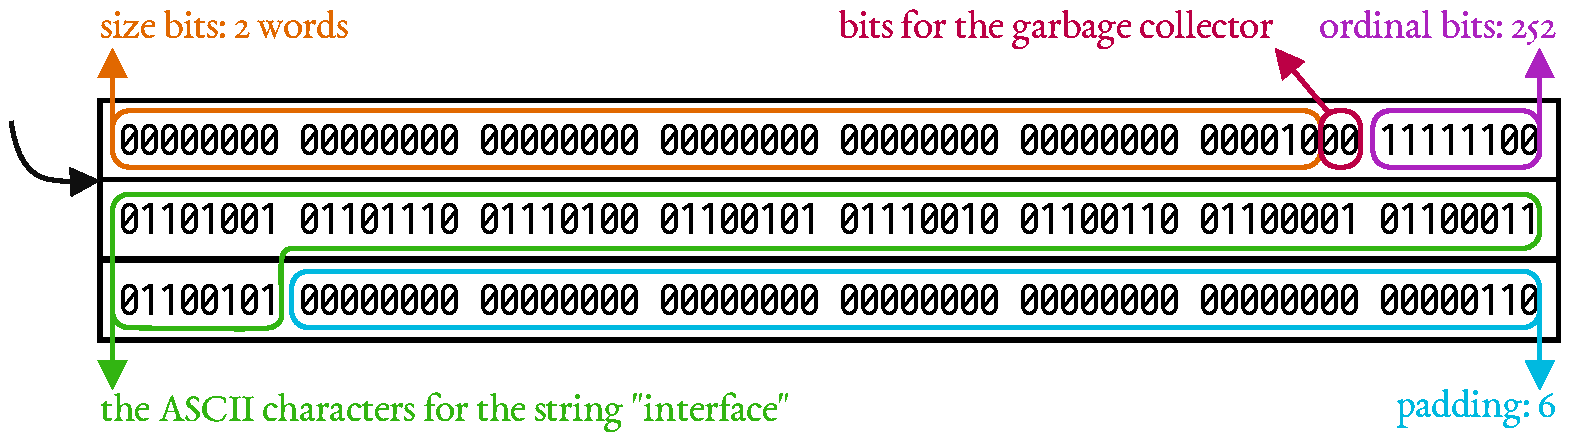
\includegraphics[scale=.55]{figures/bytestring.pdf}
\centering
\caption{The representation of the bytestring \dt{\textquotedbl{}interface\textquotedbl{}} in memory.}
\end{figure}


This string's representation consists of 3 words, one for the header and the remaining two for the characters and padding. After the header, we use one byte per ASCII character, terminated by a null byte. However, our runtime system assumes that values consist of words in memory, and our number of character bytes might not line up with the word size. We alleviate this discrepancy by filling the remaining bytes in the word with a padding. This padding consists of null bytes, with the last byte containing how many extra null bytes had to be added. If the characters and the terminating null byte perfectly fit in words, the last byte is a null byte, which serves both as the terminating byte and also the number of extra null bytes that had to be added.

The header contains the size of the string content, which is 2 words in this example. The last part of the header contains the number $252$, which is a special tag for bytestrings in OCaml. This tag indicates that none of the words in the record are pointers---none should be traversed by the garbage collector---so they don't need to use the last bit of each word to distinguish pointers from integers.

Finally, just as it is the case for all other values in our memory representation, the header is one word behind where the pointer points to.

Now that we understand how bytestrings are supposed to be represented in memory, we can start the C implementation.
We can start with defining an \kw{enum} for the possible \constructor{}s of the Coq type \ty{string}:

\begin{Verbatim}
\kw{typedef} \kw{enum} \{ \dt{EMPTYSTRING}, \dt{STRING} \} \ty{string};
\end{Verbatim}

Here is what the implementation for \fn{C.pack} looks like:

\begin{Verbatim}
\ty{value} \fn{pack}(\kw{struct} \ty{thread_info *}\tinfo{}, \ty{value} \bn{save0}) \{
  \kw{BEGINFRAME}(\tinfo{}, \dt{1})

  \cm{// Allocate enough memory}
  \ty{value} \bn{temp} = \bn{save0};
  \ty{size_t} \bn{i}, \bn{len} = \dt{0};
  \kw{while} (\fn{get_Coq_Strings_String_string_tag}(\bn{temp}) \fn{=}\fn{=} \dt{STRING}) \{
    \bn{len}\fn{+}\fn{+};
    \bn{temp} = \fn{get_args}(\bn{temp})[\dt{1}];
  \} 
  \ty{size_t} \bn{mod} = \bn{len} \fn \kw{sizeof}(\ty{value}));
  \ty{size_t} \bn{nalloc} = (\bn{len} \fn{+} \bn{pad_length}) \fn{/} \kw{sizeof}(\ty{value}) \fn{+} \dt{1ULL};
  \kw{GC_SAVE1}(\bn{nalloc})

  \ty{value *}\bn{argv} = \tinfo{}->\bn{alloc};
  \bn{argv}[\dt{0LLU}] = (\ty{value})(((\bn{nalloc} \fn{-} \dt{1}) \fn{<<} \dt{10}) \fn{+} \dt{252LLU}); \cm{// string tag}

  \cm{// Make the characters}
  \ty{char *}\bn{ptr} = (\ty{char *}) (\bn{argv} \fn{+} \dt{1LLU});
  \bn{temp} = \bn{save0};
  \kw{while} (\fn{get_Coq_Strings_String_string_tag}(\bn{temp}) \fn{==} \dt{1}) \{
    *\bn{ptr} = \fn{ascii_to_char}(\fn{get_args}(\bn{temp})[\dt{0}]);
    \bn{ptr}\fn{+}\fn{+};
    \bn{temp} = \fn{get_args}(\bn{temp})[\dt{1}];
  \}
\end{Verbatim}
\newpage
\begin{Verbatim}
  \cm{// Make the padding}
  \kw{for} (\bn{i} = \dt{0}; \bn{i} \fn{<} \fn{pad_length} \fn{-} \dt{1}; \bn{i}\fn{+}\fn{+}) \{
    \bn{ptr}[\bn{i}] = \dt{0};
  \}
  \bn{ptr}[\bn{i}] = \bn{i};

  \tinfo{}->\bn{alloc} += \bn{nalloc};
  \kw{return} (\ty{value}) (\bn{argv} \fn{+} \dt{1LLU});
  \kw{ENDFRAME}
\}
\end{Verbatim}

This function performs the following steps:
\begin{enumerate}
\item traverses the Coq \ty{string} once to compute its length, stored in \bn{len}
\item makes sure there are $n=1+\lceil (\bn{len}+1)/8\rceil$ words in the \gls{CertiCoq heap}, where it can place the bytestring
\item makes the bytestring header using the special tag and the number of words needed for the bytestring content
\item makes the character by traversing the Coq \ty{string} and converting each C \ty{char} to a Coq \ty{ascii}, by calling the \fn{ascii\_to\_char} function, which we have implemented by hand but omit here
\item makes the padding by adding null bytes, followed by how many extra null bytes had to be added
\item returns a pointer to the first character byte.
\end{enumerate}

Our implementations of \fn{C.unpack} and \fn{C.append} are similar to the implementation of \fn{C.pack} that we presented here. To summarize, \fn{C.unpack} traverses all the character bytes in the bytestring and creates \ty{ascii} and \ty{string} values, using the \gls{glue code}. \fn{C.append} computes the lengths of both of its inputs, allocates enough words in the \gls{CertiCoq heap}, copies characters, and adds padding.

\subsection{The Functional Model}

The simplest way to model bytestrings in Coq is to define them as Coq \ty{string}s. This makes the \gls{functional model}s of all the functions that operate of our \gls{foreign type} trivial:

\begin{Verbatim}
\kw{Module} \ty{FM}.
  \kw{Definition} \ty{bytestring} : \ty{Type} := \ty{string}.
  \kw{Definition} \fn{pack} (\bn{x} : \ty{string}) : \ty{bytestring} := \bn{x}.
  \kw{Definition} \fn{unpack} (\bn{x} : \ty{bytestring}) : \ty{string} := \bn{x}.
  \kw{Definition} \fn{append} (\bn{x} \bn{y} : \ty{bytestring}) : \ty{bytestring} := \fn{append} \bn{x} \bn{y}.
\kw{End} \ty{FM}.
\end{Verbatim}

A curious reader might wonder why we did not address the length of the bytestring in our \gls{functional model}. This would be a fair question, given that we \emph{have} addressed a similar restriction in the \gls{functional model} for integers, in \autoref{integers}. Our answer in this case is practicality. In the memory representation above, we showed that the bytestring header contains 54 bits (in a 64-bit setting) for the size of the string, in words. Thus, the largest bytestring we can create will have $(2^{54})\cdot{}8$, or $2^{57}$ bytes, which is $128$ petabytes.
For \fn{C.pack}, we would need to start with a Coq \ty{string}. In order to reach a bytestring that is $128$ petabytes, at $2$ words per record, we would need $2\cdot{}8\cdot{}2^{57} = 2^{61}$ bytes of memory, i.e.\ $\approx{}2.3$ exabytes.\footnote{This question and its answer was observed by Appel.}  Here we are assuming we are not going to run Coq functions on memories that large, but it is also possible to design a \gls{functional model} for bytestrings in a way that would account for the maximum length.\footnote{In such a design, the \fn{pack} function would have decide how to treat the inputs that would create bytestrings larger than what the bytestring representation could handle. The \fn{pack} function could choose to return only the part that fits in memory, or it could choose to return an \ty{option} value, etc.}

We will not present any proofs about the models for the \gls{foreign function}s on \ty{bytestring}s since our model is trivial and all proofs will simply be about Coq \ty{string}s.
\section{Printing Bytestrings}
\label{printingbytestrings}

% https://stackoverflow.com/questions/57758951/what-are-freer-monads
% https://okmij.org/ftp/Haskell/extensible/more.pdf
% http://lambda-the-ultimate.org/node/92
% https://sf.snu.ac.kr/publications/itrees.pdf

So far, we have only implemented pure \gls{foreign function}s. Neither integers nor bytestrings have any side effects; functions that operate on them are guaranteed to return the same result every time they use the same arguments,\footnote{As long as there is enough space in the \gls{CertiCoq heap}. If not, garbage collection will fail with an error.} with no observable difference from the outside. Real programs, however, often need to have side effects, therefore we need to find a way to write effectful programs if we want to be able to express them.

Two factors require us to keep the language pure even when expressing effectful programs. The first factor is that Coq does not have a default evaluation order, since its underlying type theory enjoys strong normalization and confluence~\cite{coquand1985, werner1994}. The second factor is that we use our functions in proofs and types, and we do not want proofs and types to depend on the outside world.

Thankfully, we are not the first to face this conundrum. The Haskell community has encountered the same question from the beginning; in their case, Haskell's lazy evaluation made it difficult to predict when a function's side effect would be executed. Their solution was to forbid functions from having side effects\footnote{As noted in the famous XKCD comic:\\``Code written in Haskell is guaranteed to have no side effects." ``... because no one will ever run it?"~\cite{xkcd:haskell}} and to exile all side effects into the \ty{IO} monad. Effectful programs are then expressed as terms with an \ty{IO} type, \parametrized{} by the result type of the computation. For example, here are the Haskell terms that we use for printing to and scanning from the console:

\begin{Verbatim}
\fn{putStrLn} :: \ty{String} -> \ty{IO} \ty{String}
\fn{getLine} :: \ty{IO} \ty{String}
\end{Verbatim}

Neither of these terms have side effects by themselves; they are merely \emph{action}s that we can use to build a program. The user composes these actions using the monadic bind to build larger programs. Here is an example Haskell program, written as a chain of monadic actions (without syntactic sugar, i.e.\ \kw{do} notation):

\begin{Verbatim}
\fn{main} :: \ty{IO ()}
\fn{main} = \fn{getLine} \fn{>}\fn{>}\fn{=} (\textbackslash{}\bn{x} -> \fn{putStrLn} (\dt{"Hello "} \fn{+}\fn{+} \bn{x}))
\end{Verbatim}

This program, when executed, reads a line of user input from the console, prepends the input string with another string, and prints the new string. What triggers the execution, however, is the runtime: Haskell's runtime is hard-coded to execute the \fn{main} action when the program starts. The runtime has an interpreter for actions, which executes the left side of the bind, plugs the result in the function on the right side of the bind, and keeps interpreting. This design allows us to express effectful programs purely (since actions are values that do not have side effects before execution), provides explicit sequencing for effectful computations, and makes the execution order of effects predictable.

We want to express effectful programs the same way in Coq, for which we will have to write an interpreter for actions in C.

In this section, we will extend our \glslink{foreign type}{foreign} bytestring implementation from the previous section with a monad that has effectful actions to print bytestrings into a stream and to scan (read) bytestrings from a stream. The VST proofs for these functions will be addressed in future work.

\subsection{The Coq Interface}

Our interface will have to contain a monadic type \ty{M}, a function \fn{pure} to inject pure values into our monad (also called returning), and a function \fn{bind} to express an effect followed by more computation or effects. We also expect functions in the interface that express effects, such as \fn{print} for printing and \fn{get\_line} for taking inputs. Here is what that interface looks like as a \kw{Module Type}:

\begin{Verbatim}
\kw{Module Type} \ty{Bytestring}.
  \cm{(* Definitions from the previous version of \ty{Bytestring} *)}
  \kw{Parameter} \ty{M} : \ty{Type} -> \ty{Type}.
  \kw{Parameter} \fn{pure} : \kw{forall} \{\bn{A} : \ty{Type}\}, \bn{A} -> \ty{M} \bn{A}.
  \kw{Parameter} \fn{bind} : \kw{forall} \{\bn{A} \bn{B} : \ty{Type}\}, \ty{M} \bn{A} -> (\bn{A} -> \ty{M} \bn{B}) -> \ty{M} \bn{B}.
  \kw{Parameter} \fn{print} : \ty{bytestring} -> \ty{M} \ty{unit}.
  \kw{Parameter} \fn{get_line} : \ty{M} \ty{bytestring}.
  \kw{Parameter} \ty{same_behavior} : \kw{forall} \{\bn{A} : \ty{Type}\}, \ty{M} \bn{A} -> \ty{M} \bn{A} -> \ty{Prop}.
\kw{End} \ty{Bytestring}.
\end{Verbatim}

Notice that we have an additional element in this module type, called \ty{same\_behavior}. We will use this relation later in \autoref{modelproofseffects} to reason about actions, to assert that two actions have the same behavior.


Following the recipe we demonstrated in the previous examples, we want to implement a \ty{C} module of the module type \ty{Bytestring}. Until now, the \ty{C} modules we have seen have consisted of \kw{Axiom}s. These axioms were only realized when a Coq program that uses them is compiled to C and the compiled program is linked to the C file containing the \gls{foreign function}s. We will, however, diverge from this recipe now.

Just like how we would design a abstract syntax tree (AST) in Coq for an interpreter in Coq, we will design an AST in Coq for an interpreter in C. The user will write their programs using this AST, and compile them. The interpreter for this AST, which is written by the user of our \ffi{}, will be called from the C wrapper file described in \autoref{usage}.

\begin{Verbatim}
\kw{Module} \ty{C} <: \ty{Bytestring}.
  \cm{(* Definitions from the previous version of \ty{C} for bytestrings *)}

  \kw{Inductive} \ty{MI} : \ty{Type} -> \ty{Type} :=
  | \dt{pureI} : \kw{forall} \{\bn{A} : \ty{Type}\}, \bn{A} -> \ty{MI} \bn{A}
  | \dt{bindI} : \kw{forall} \{\bn{A} \bn{B} : \ty{Type}\}, \ty{MI} \bn{A} -> (\bn{A} -> \ty{MI} \bn{B}) -> \ty{MI} \bn{B}
  | \dt{printI} : \ty{bytestring} -> \ty{MI} \ty{unit}
  | \dt{get_lineI} : \ty{MI} \ty{bytestring}.

  \kw{Definition} \ty{M} : \ty{Type} -> \ty{Type} := \ty{MI}.
  \kw{Definition} \fn{pure} : \kw{forall} \{\bn{A} : \ty{Type}\}, \bn{A} -> \ty{M} \bn{A} := @\dt{pureI}.
  \kw{Definition} \fn{bind} : \kw{forall} \{\bn{A} \bn{B} : \ty{Type}\}, \ty{M} \bn{A} -> (\bn{A} -> \ty{M} \bn{B}) -> \ty{M} \bn{B} := @\dt{bindI}.
  \kw{Definition} \fn{print} : \ty{bytestring} -> \ty{M} \ty{unit} := @\dt{printI}.
  \kw{Definition} \fn{get_line} : \ty{M} \ty{bytestring} := @\dt{get_lineI}.

  \kw{Axiom} \ty{same_behavior} : \kw{forall} \{\bn{A} : \ty{Type}\}, \ty{M} \bn{A} -> \ty{M} \bn{A} -> \ty{Prop}.
\kw{End} \ty{C}.
\end{Verbatim}

We define here an \gls{inductive type}\footnote{If we wanted to express possibly nonterminating programs, we could have described the free monad as a \emph{coinductive} type. Other than having to force the thunk explicitly from the C side, not much would have changed operationally. \citeauthor{abel2017interactive}~\cite{abel2017interactive} explore a coinductive \ty{IO} monad for Agda, which we could base a similar Coq system on.} that has \constructor{}s for both the monadic components (such as returning and binding) and the effectful \gls{foreign function}s. We then provide aliases for these \constructor{}s, because Coq modules do not allow us to use \constructor{}s to satisfy the requirements of a \kw{Module Type}. Finally, we axiomatize \ty{same\_behavior}, which will only make sense when we have a \gls{functional model} for it.

With this interface, we can write the same Haskell function now in Coq:

\begin{Verbatim}
\kw{Definition} \fn{main} : \ty{C.M unit} :=
  \fn{C.bind} \fn{C.get_line} (\kw{fun} \bn{x} => \fn{C.print} \bn{x}).
\end{Verbatim}

\subsection{The C Implementation}
\label{printingbytestringsc}

Another way we have diverged from the usual recipe is the lack\footnote{We still use \kw{CertiCoq Register} for \fn{C.pack}, \fn{C.unpack}, and \fn{C.append} on bytestrings.} of the use of \kw{CertiCoq Register} to register any of our effectful functions. This is a deliberate choice on our part; we will implement a function \fn{runM} that executes an action, and \fn{runM} will be called in the C wrapper file after computing the program result. We define \fn{runM} as such:

\begin{Verbatim}
\kw{typedef enum} \{ \dt{PURE}, \dt{BIND}, \dt{PRINT}, \dt{GETLINE} \} \ty{M};

\ty{value} \fn{runM}(\kw{struct} \ty{thread_info *}\tinfo{}, \ty{value} \bn{action}) \{
  \kw{BEGINFRAME}(\tinfo{}, \dt{2})
  \kw{switch} (\fn{get_prog_C_MI_tag}(\bn{action})) \{
    \kw{case} \dt{PURE}:
      \kw{return} \fn{get_args}(\bn{action})[\dt{1}];
    \kw{case} \dt{BIND}: \{
      \ty{value} \bn{arg0} = \fn{get_args}(\bn{action})[\dt{2}];
      \ty{value} \bn{arg1} = \fn{get_args}(\bn{action})[\dt{3}];
      \ty{value} \bn{temp} = \kw{LIVEPOINTERS1}(\tinfo{}, \fn{runM}(\tinfo{}, \bn{arg0}), \bn{arg1});
      \bn{temp} = \fn{call}(\tinfo{}, \bn{arg1}, \bn{temp});
      \kw{return} \fn{runM}(\tinfo{}, \bn{temp});
    \}
    \kw{case} \dt{PRINT}: \{
      \ty{value} \bn{arg0} = \fn{get_args}(\bn{action})[\dt{0}];
      \fn{print_bytestring}(\bn{s});
      \kw{return} \fn{make_Coq_Init_Datatypes_unit_tt}();
    \}
    \kw{case} \dt{GETLINE}:
      \kw{return} \fn{get_line_bytestring}(\tinfo{});
    \kw{default}:
      \kw{return} \dt{0};
  \}
  \kw{ENDFRAME}
\}
\end{Verbatim}

\newpage
We start by defining a C \kw{enum} that makes it easier to understand what \constructor{} of \ty{C.MI} is handled, and then move on to the \fn{runM} function. \fn{runM} traverses the action AST that was built on the Coq side and returns the value inside the monad. The \dt{PURE} case is simple; we just return the argument in the constructor.\footnote{Note that the \dt{0}\textsuperscript{th} index in the array returned by \fn{get\_args} will contain the type argument for \dt{MI.pureI}.} The \dt{PRINT} and \dt{GETLINE} cases are simple to interpret, although here we elide the \fn{print\_bytestring} and \fn{get\_line\_bytestring} functions, where the complexity of these cases is hidden.

The \dt{BIND} case is at the crux of our interpreter for monadic actions. We collect the monadic action and the continuation function from the \dt{MI.bindI} constructor. Then, we have to execute the monadic action to obtain the input of the continuation function, which we achieve with a recursive call to \fn{runM}. When executing this monadic action, we have to keep in mind that \bn{arg1} is not in the roots, and it should be protected if our recursive call ultimately calls the garbage collector. Once we know what input to call the continuation function with, we can \fn{call} it. The continuation function returns another monadic action, which we can pass to another recursive call to \fn{runM}.

This function currently uses the C call stack to handle recursion. To avoid stack overflow errors, we can choose to implement \fn{runM} with an explicit call stack, or we can try to rewrite the action input of \fn{runM} using the associativity law of monads~\cite{wadler1992essence}, where \code{\fn{C.bind} (\fn{C.bind} \bn{m} \bn{f}) \bn{g}}\, can be rewritten to \code{\fn{C.bind} \bn{m} (\kw{fun} \bn{x} \code{=}\code{>} \fn{C.bind} (\bn{f} \bn{x}) \bn{g})}. Repeated applications of such rewrites can ensure that the action argument to \fn{C.bind} is atomic, after which we only need tail recursion to execute the remaining action. We leave this implementation detail to the users of our \ffi{}.

\subsection{The Functional Model}

Following the Haskell tradition~\cite{peytonjones1993imperative}, we define the \gls{functional model} of our effectful monads as a function from the state to a pair of a result and the new state. For our particular set of effects, where we only write to the console and read from the console, we model the program state as the input stream to the program and the output stream from the program. The rest of our \gls{functional model} definitions mirror the purely functional state monad~\cite{jones1995functional}.

\begin{Verbatim}
\kw{Module} \ty{FM} <: \ty{Bytestring}.
  \cm{(* Definitions from the previous version of \ty{FM} for bytestrings *)}

  \kw{Definition} \ty{state} : \ty{Type} :=
    (\ty{string} \ty{*} \ty{string}). \cm{(* the input stream and the output stream *)}
  \kw{Definition} \ty{M} (\bn{A} : \ty{Type}) : \ty{Type} := \ty{state} -> \bn{A} \ty{*} \ty{state}.
  \kw{Definition} \fn{pure} \{\bn{A} : \ty{Type}\} (\bn{a} : \bn{A}) : \ty{M} \bn{A} := \kw{fun} \bn{s} => (\bn{a}, \bn{s}).
  \kw{Definition} \fn{bind} \{\bn{A} \bn{B} : \ty{Type}\} (\bn{m} : \ty{M} \bn{A}) (\bn{f} : \bn{A} -> \ty{M} \bn{B}) : \ty{M} \bn{B} :=
    \kw{fun} \bn{s} => \kw{let} '(\bn{a}, \bn{s'}) := \bn{m} \bn{s} \kw{in} \bn{f} \bn{a} \bn{s'}.

  \kw{Definition} \fn{print} (\bn{x} : \ty{bytestring}) : \bn{M} \ty{unit} :=
    \kw{fun} '(\bn{input}, \bn{output}) => (\dt{tt}, (\bn{input}, \fn{append} \bn{output} \bn{x})).

  \kw{Definition} \fn{get_line} : \ty{M} \ty{bytestring} :=
    \kw{fun} '(\bn{input}, \bn{output}) => (\fn{substring} \dt{0} \bn{n} \bn{input},
        (\fn{substring} \bn{n} (\fn{length} \bn{input}) \bn{input}, \bn{output})).

  \kw{Definition} \fn{same_behavior} {\bn{A}} (\bn{a1} \bn{a2} : \ty{M} \bn{A}) : \ty{Prop} :=
    \kw{forall} (\bn{s} : \ty{state}), \bn{a1} \bn{s} \ty{=} \bn{a2} \bn{s}.
\kw{End} \ty{FM}.
\end{Verbatim}

Before we move on to the proofs about our \gls{functional model}, let us observe our \fn{same\_behavior} definition above. We left its definition as an axiom in the \ty{C} module with no intention of realizing its definition on the C side, but we are actually providing a Coq definition in the \gls{functional model}. We do not need to provide a definition in the \ty{C} module; \fn{same\_behavior} returns a \ty{Prop}, which is erased by CertiCoq. Therefore \fn{same\_behavior} itself never has computationally relevant content. In \ty{FM}, however, we need a real definition so that we can later rewrite the uses of \ty{C.same\_behavior} into \ty{FM.same\_behavior} and proceed with the proof.

\subsection{Model Proofs for Foreign Functions}
\label{modelproofseffects}

In the previous examples of the \ffi{}, we have used Coq's equality type \ty{=} to claim equalities between values of a \gls{foreign type}. Unfortunately, this approach does not make sense for effectful actions; these values are ASTs of actions and the equality of the AST is not correlated with the equality of the output when the actions are executed. It is possible for two action ASTs to be different and have the same output when executed, just as it is possible for two ASTs to be the same and have different outputs. Therefore, we will use the \fn{same\_behavior} relation that we included in our interface.

\begin{Verbatim}
\kw{Section} \ty{BytestringProofs}.

\cm{(* Generation of foreign function descriptions. *)}
\kw{Parameter} \fn{pure_spec}.
\kw{Parameter} \fn{bind_spec}.
\kw{Parameter} \fn{print_spec}.
\kw{Parameter} \fn{get_line_spec}.
\kw{Parameter} \fn{same_behavior_spec}.
\end{Verbatim}

We use the mechanisms in \autoref{genspecprim} and \autoref{modelspec} to set ourselves up to rewrite functions from \ty{C} to their \ty{FM} counterparts. We are now ready to prove a simple result about printing bytestrings, following a similar idea to that of \citeauthor{swierstra2007beauty}~\cite{swierstra2007beauty}, who provide a functional semantics for the ``awkward squad" to reason about impure code:
\newpage
\begin{Verbatim}
\kw{Theorem} \fn{print_steps} :
  \kw{forall} (\bn{a} \bn{b} : \ty{C.bytestring}),
    \ty{C.same_behavior} (\fn{C.bind} (\fn{C.print} \bn{a}) (\kw{fun} _ => \fn{C.print} \bn{b}))
                    (\fn{C.print} (\fn{C.append} \bn{a} \bn{b})).
\kw{Proof}.
  \tc{intros} \bn{a} \bn{b}.

  \tc{eapply} (\fn{transport} \fn{id}). \tc{symmetry}.
  \tc{eapply} (\fn{same_behavior_spec} \ty{unit}); \tc{simpl}.
  \tc{foreign_rewrites}.
  \tc{unfold} \ty{FM.same_behavior}.

  \tc{props} \fn{bind_spec}.
  \tc{foreign_rewrites}.
  \tc{unfold} \fn{FM.bind}.

  \tc{props} \fn{print_spec}.
  \tc{foreign_rewrites}.
  \tc{unfold} \fn{FM.print}.

  \tc{props} \fn{append_spec}.
  \tc{foreign_rewrites}.
  \tc{unfold} \fn{FM.append}.

  \tc{intros} [\bn{instream} \bn{outstream}].
  \tc{rewrite} \fn{append_assoc}; \tc{auto}.
\kw{Qed}.

\kw{End} \ty{BytestringProofs}.
\end{Verbatim}

We provide the type argument \ty{unit} to \fn{same\_behavior\_spec}, since our example program has the type \ty{C.M unit}. Then we rewrite \ty{C} terms to their \ty{FM} counterparts, unfold the \ty{FM} definitions, and finish the proof.

Unlike the model proof in \autoref{integers}, our model proof on monadic effects does not let us rewrite a theorem statement about functions from \ty{C} into a theorem statement about functions from \ty{FM} all at once. Since the rest of the monadic action depends on the result of the continuation, we can only rewrite and unfold one step at a time. Once the \gls{functional model} definition of the continuation is evaluated, we can rewrite and unfold it once again.
\section{Mutable Arrays}
\label{mutablearrays}

Purely functional data structures are easier to reason about than imperative data structures. However, they are inherently inefficient for some use cases~\cite{ponder1988applicative, amram1992pointers, pippenger96pure, okasaki1999purely}, therefore we inevitably need mutable data structures.

Mutable data structures à la OCaml break purity, which is why we only want to allow them in a controlled way. One way to implement them without breaking purity is, of course, to implement them as an effect, similar to how we printed bytestrings in \autoref{printingbytestrings}. However, this may be more restricting than we need. As \citeauthor{launcybury1994lazy}~\cite{launcybury1994lazy} have demonstrated for the \ty{ST} monad in Haskell, it is possible to have local mutation that is externally pure. That is, a client of our function with local mutation cannot tell if our function has mutation in it; its type is pure and it returns the same value for the same inputs.

In this section, we will implement a monad to use mutable arrays as a \gls{foreign type} in Coq, and functions to set, get, and run the monad as \gls{foreign function}s. The VST proofs for these functions will be addressed in future work.

\subsection{The Coq Interface}

Here we will follow a similar approach to how we handled effects in \autoref{printingbytestrings}, but we can now expose \fn{runM} to the Coq side, since we can model the mutation in a purely functional way and it does not break purity.

\begin{Verbatim}
\kw{Definition} \ty{elt} := \ty{nat}.

\kw{Module Type} \ty{Array}.
  \kw{Parameter} \ty{M} : \ty{Type} -> \ty{Type}.
  \kw{Parameter} \fn{pure} : \kw{forall} \{\bn{A} : \ty{Type}\}, \bn{A} -> \ty{M} \bn{A}.
  \kw{Parameter} \fn{bind} : \kw{forall} \{\bn{A} \bn{B} : \ty{Type}\}, \ty{M} \bn{A} -> (\bn{A} -> \ty{M} \bn{B}) -> \ty{M} \bn{B}.
  \kw{Parameter} \fn{set} : \ty{nat} -> \ty{elt} -> \ty{M} \ty{unit}.
  \kw{Parameter} \fn{get} : \ty{nat} -> \ty{M} \ty{elt}.
  \kw{Parameter} \fn{runM} : \kw{forall} \{\bn{A} : \ty{Type}\} (\bn{len} : \ty{nat}) (\bn{init} : \ty{elt}), \ty{M} \bn{A} -> \bn{A}.
\kw{End} \ty{Array}.
\end{Verbatim}

Once again, we have monadic components for returning and binding, as well as ``effectful" operations on arrays, such as getting and setting. The main difference is the \fn{runM} function, which takes the length of the initial array and the initial value at unset indices of the array.

Our approach here is different from that of \citeauthor{launcybury1994lazy} in that we do not apply their rank-2 types trick for the \ty{ST} monad, which restricts references from escaping the monad. Instead, we never expose a reference to a mutable variable (or the entire array) from the interface. The user will have only one array in each instance of the monad \ty{M}.\footnote{Users can have multiple arrays using a monad stack.} While our interface here looks similar to that of \citeauthor{sakaguchi2020program}~\cite{sakaguchi2020program}, our approach here is simpler and less type-safe.\footnote{For \fn{C.set}, we ignore the operation if the index is out of bounds. For \fn{C.get}, we return the default element if the index is out of bounds.} This is a deliberate design choice to make the proof simpler to present.

\begin{Verbatim}
\kw{Module} \ty{C} <: \ty{Array}.
  \kw{Inductive} \ty{MI} : \ty{Type} -> \ty{Type} :=
  | \dt{pureI} : \kw{forall} \{\bn{A} : \ty{Type}\}, \bn{A} -> \ty{MI} \bn{A}
  | \dt{bindI} : \kw{forall} \{\bn{A} \bn{B} : \ty{Type}\}, \ty{MI} \bn{A} -> (\bn{A} -> \ty{MI} \bn{B}) -> \ty{MI} \bn{B}
  | \dt{setI} : \ty{nat} -> \ty{elt} -> \ty{MI} \ty{unit}
  | \dt{getI} : \ty{nat} -> \ty{MI} \ty{elt}.

  \kw{Definition} \ty{M} := \ty{MI}.
  \kw{Definition} \fn{pure} : \kw{forall} \{\bn{A} : \ty{Type}\}, \bn{A} -> \ty{M} \bn{A} := @\dt{pureI}.
  \kw{Definition} \fn{bind} : \kw{forall} \{\bn{A} \bn{B} : \ty{Type}\}, \ty{M} \bn{A} -> (\bn{A} -> \ty{M} \bn{B}) -> \ty{M} \bn{B} := @\dt{bindI}.
  \kw{Definition} \fn{set} : \ty{nat} -> \ty{elt} -> \ty{M} \ty{unit} := @\dt{setI}.
  \kw{Definition} \fn{get} : \ty{nat} -> \ty{M} \ty{elt} := @\dt{getI}.
  \kw{Axiom} \fn{runM} : \kw{forall} {\bn{A}} (\bn{len} : \ty{nat}) (\bn{init} : \ty{elt}), \ty{M} \bn{A} -> \bn{A}.
\kw{End} \ty{C}.
\end{Verbatim}

Similar to \autoref{printingbytestrings}, we implement operations in the mutable array monad as an abstract syntax tree of actions. We will still have a \fn{runM} function in C to interpret these actions, but this time, we will expose it to the Coq side by declaring it an \kw{Axiom} and telling the compiler that this axiom is realized by a particular C function.

\begin{Verbatim}
\kw{CertiCoq Register} [ \fn{C.runM} => \dt{"runM"} \kw{with tinfo} ] \kw{Include} [ \dt{"prims.h"} ].
\end{Verbatim}

\subsection{The C Implementation}

We implement the C side of the mutable array monad interpreter with two functions: \fn{runM} allocates the necessary space on the \gls{CertiCoq heap} and initializes the array with the initial value at each index. \fn{executeM} traverses the monadic action and executes it.

\begin{Verbatim}
\ty{value} \fn{runM}(\kw{struct} \ty{thread_info *}\tinfo{}, \ty{value} \bn{a}, \ty{value} \bn{len},
                 \ty{value} \bn{save0}, \ty{value} \bn{save1}) \{
  \kw{BEGINFRAME}(\tinfo{}, \dt{2})
  \ty{size_t} \bn{size} = \fn{nat_to_size_t}(\bn{len});
  \bn{nalloc} = \bn{size} \fn{+} \dt{1}; \kw{GC_SAVE2}
  \ty{value *}\bn{arr} = \tinfo{}->\bn{alloc};
  \bn{arr}[\dt{0LLU}] = \bn{size} \fn{<<} \dt{10};
  \bn{arr} = \bn{arr} \fn{+} \dt{1LLU};
  \kw{for} (\ty{size_t} \bn{i} = \dt{0}; \bn{i} \fn{<} \bn{size}; \bn{i}\fn{++}) \{
    \bn{arr}[\bn{i}] = \bn{save0};
  \}
  \tinfo{}->\bn{alloc} \fn{+}= \bn{nalloc};
  \kw{return} \fn{executeM}(\tinfo{}, \bn{size}, \bn{save0}, (\ty{value}) \bn{arr}, \bn{save1});
  \kw{ENDFRAME}
\}
\end{Verbatim}

The function first converts\footnote{The implementation of \fn{nat\_to\_size\_t} is almost the same as \fn{uint63\_from\_nat}, just without the bit shifting to make the last bit \dt{1}.} the array length \bn{len}, which is a Coq \ty{nat}, to a C \ty{size\_t}. This number determines how much space we need to allocate on the \gls{CertiCoq heap}. We treat the array like a Coq constructor with that many arguments, we allocate one word for the header and one word per array index. Of course, while we perform a memory check and possibly call the garbage collector, we have to make sure the initial value for the array (\bn{save0}) and the monadic action (\bn{save1}) are not collected by accident, therefore we save them in a stack frame using the \kw{GC\_SAVE} macro.
Once we have enough space, we initialize the array with the initial value \bn{save0}, and call \fn{executeM} to execute the monadic action.

\begin{Verbatim}
\kw{typedef enum} \{ \dt{PURE}, \dt{BIND}, \dt{SET}, \dt{GET} \} \ty{M};

\ty{value} \fn{executeM}(\kw{struct} \ty{thread_info *}\tinfo{}, \ty{size_t} \bn{size}, 
           \ty{value} \bn{init}, \ty{value} \bn{save0}, \ty{value} \bn{save1}) \{
  \kw{BEGINFRAME}(\tinfo{}, \dt{2})
  \kw{switch} (\fn{get_prog_C_MI_tag}(\bn{save1})) \{
    \cm{// Cases for \dt{PURE} and \dt{BIND} as before}
    \kw{case} \dt{SET}: \{
      \ty{value} \bn{arg0} = \fn{get_args}(\bn{save1})[\dt{0}];
      \ty{size_t} \bn{i} = \fn{nat_to_size_t}(\bn{arg0});
      \kw{if} (\bn{i} \fn{<} \bn{size}) \{
        \bn{nalloc} = \dt{1}; \kw{GC_SAVE2}
        \ty{value} \bn{arg1} = \fn{get_args}(\bn{save1})[\dt{1}];
        \fn{certicoq_modify}(\tinfo{}, (\ty{value *}) \bn{save0} \fn{+} \bn{i}, \bn{arg1});
      \}
      \kw{return} \fn{make_Coq_Init_Datatypes_unit_tt}();
    \}
    \kw{case} \dt{GET}: \{
      \ty{value} \bn{arg0} = \fn{get_args}(\bn{save1})[\dt{0}];
      \ty{size_t} \bn{i} = \fn{nat_to_size_t}(\bn{arg0});
      \kw{if} (\bn{i} \fn{<} \bn{size}) \{
        \kw{return} \fn{get_args}(\bn{save0})[\bn{i}];
      \} \kw{else} \{
        \kw{return} \bn{init};
      \}
    \}
  \}
  \kw{ENDFRAME}
\}
\end{Verbatim}

Our \fn{executeM} implementation is similar to the \fn{runM} implementation in \autoref{printingbytestringsc}; it is a free monad interpreter written in C. We omit the \dt{PURE} and \dt{BIND} cases here since they are almost the same as the previous interpreter.
The \dt{SET} and \dt{GET} cases, however, are interesting.

When we see a \dt{SET} action, we want to find the right slot in the array and assign the new value in that slot. However, we have to notify the garbage collector that we have a mutable reference, because the garbage collector normally operates on the assumption that older values never point on the newer values, which allows it to move values around freely and erase unused values~\cite{fenichel1969lisp}. By creating a mutable reference, we break that assumption, therefore we have to keep a remembered set of old values pointing to new values, so that the garbage collector can update these references when new values are moved~\cite{sansom1993generational}. We achieve that with a call to \fn{certicoq\_modify}\footnote{\fn{certicoq\_modify} was implemented by Tim Carstens and Appel.}, which is a write barrier that saves the mutable reference to the bottom end of the \gls{CertiCoq heap} and therefore keeps a remembered set. 

When we see a \dt{GET} action, we simply access the index in the array if it is within bounds, or return the default value of all indices if the index is out of bounds.

\paragraph*{Reuse in Persistent Arrays} While the design of our array interface and its \gls{foreign function}s is for mutable arrays, it is possible to use the same memory representation of arrays for persistent arrays, which are recently introduced to the Coq standard library~\cite{conchon2007persistent, denes2013towards}.

\subsection{The Functional Model}

The \gls{functional model} for our mutable array monad is similar to our \gls{functional model} for effects in \autoref{printingbytestrings}, except we also provide an implementation for \fn{runM}, which interprets the abstract syntax trees of actions in a purely functional way.

\begin{Verbatim}
\kw{Module} \ty{FM} <: \ty{Array}.
  \kw{Definition} \ty{state} : \ty{Type} :=
    (\ty{list} \ty{elt} \ty{*} \ty{elt}). \cm{(* the internal list and the default element *)}
  \kw{Definition} \ty{M} (\bn{A} : \ty{Type}) : \ty{Type} := \ty{state} -> \ty{A} \ty{*} \ty{state}.
  \kw{Definition} \fn{pure} \{\bn{A} : \ty{Type}\} (\bn{a} : \bn{A}) : \ty{M} \bn{A} := \kw{fun} \bn{s} => (\bn{a}, \bn{s}).
  \kw{Definition} \fn{bind} \{\bn{A} \bn{B} : \ty{Type}\} (\bn{m} : \ty{M} \bn{A}) (\bn{f} : \bn{A} -> \ty{M} \bn{B}) : \ty{M} \bn{B} :=
    \kw{fun} \bn{s} => \kw{let} '(\bn{a}, \bn{s'}) := \bn{m} \bn{s} \kw{in} \bn{f} \bn{a} \bn{s'}.
  \kw{Definition} \fn{set} (\bn{index} : \ty{nat}) (\bn{x} : \ty{elt}) : \ty{M} \ty{unit} :=
    \fn{fun} '(\bn{l}, \bn{init}) => (\dt{tt}, (\fn{replace_nth} \bn{index} \bn{l} \bn{x}, \bn{init})).
  \kw{Definition} \fn{get} (\bn{index} : \ty{nat}) : \ty{M} \ty{elt} :=
    \kw{fun} '(\bn{l}, \bn{init}) => (\fn{nth} \bn{index} \bn{l} \bn{init}, (\bn{l}, \bn{init})).
  \kw{Definition} \fn{runM} \{\bn{A} : \ty{Type}\} (\bn{len} : \ty{nat}) (\bn{init} : \ty{elt}) (\bn{m} : \ty{M} \bn{A}) : \bn{A} :=
    \fn{fst} (\bn{m} (\fn{repeat} \bn{init} \bn{len}, \bn{init})).
\kw{End} \ty{FM}.
\end{Verbatim}

\subsection{Model Proofs for Foreign Functions}

In \autoref{modelproofseffects}, we argued that using Coq's equality type \ty{=} does not make sense for effectful actions, since the output of the execution depends on the outside world. In our mutable array monad, however, the output does not depend on the outside world, and we do not break purity by calling \fn{runM} to execute the monadic action. Therefore, we can call \fn{C.runM} on both sides of the equality, and as long as the array size and default value are the same, we can argue that two different actions have the same result.

In the example below, we prove that first \fn{set}ting an index of an array to a value and then \fn{get}ting the value at that index, gives the same final result (but not the same state). Our proof once again resembles that of \citeauthor{swierstra2007beauty}~\cite{swierstra2007beauty}, since we use the functional semantics in \ty{FM} to reason about mutable state:

\begin{Verbatim}
\kw{Lemma} \fn{set_get} :
  \kw{forall} (\bn{n} \bn{len} : \ty{nat}) (\bn{bound} : \bn{n} \ty{<} \bn{len}) (\bn{init} : \ty{elt}) (\bn{to_set} : \ty{elt}),
    (\fn{C.runM} \bn{len} \bn{init} (\fn{C.bind} (\fn{C.set} \bn{n} \bn{to_set}) (\kw{fun} _ => \fn{C.get} \bn{n})))
      \ty{=}
    (\fn{C.runM} \bn{len} \bn{init} (\fn{C.pure} \bn{to_set})).
\kw{Proof}.
  \tc{intros} \bn{n} \bn{len} \bn{bound} \bn{init} \bn{to_set}.

  \tc{props} \fn{runM_spec}.
  \tc{foreign_rewrites}.
  \tc{unfold} \fn{FM.runM}.

  \tc{props} \fn{bind_spec}.
  \tc{props} \fn{pure_spec}.
  \tc{foreign_rewrites}.
  \tc{unfold} \fn{FM.bind}, \fn{FM.pure}.

  \tc{props} \fn{set_spec}.
  \tc{props} \fn{get_spec}.
  \tc{foreign_rewrites}.

  \tc{eapply} \fn{nth_replace_nth}.
  \tc{rewrite} \fn{repeat_length}.
  \tc{auto}.
\kw{Qed}.
\end{Verbatim}

Similar to \autoref{modelproofseffects}, we have to rewrite and unfold the \ty{C} functions one at a time, since the second argument of \fn{C.bind}, the continuation, hides more uses of functions from \ty{C} inside. Once the \gls{functional model} definition of the continuation is evaluated, we continue rewriting and unfolding as necessary and finally finish the proof by reasoning about the \gls{functional model} definitions \fn{FM.set} and \fn{FM.get}.
\addtocontents{toc}{\protect\newpage}
\chapter{Related Work}
\label{related}

\epigraph{Comparison is the thief of all joy.}{Theodore Roosevelt, in a letter to W.S. Bigelow, 1898}
% Roosevelt, in a letter to William Sturgis Bigelow on March 29, 1898: "The phrase, “Comparison is the thief of all joy’ evokes a powerful sentiment that can be life-changing. If we compare ourselves to others, we may be left with feelings of inferiority or superiority—and neither creates an emotionally healthy human being!"

Some of the main contributions of this dissertation, as well as the examples presented in \autoref{examples}, build upon preexisting work in the literature. In this section, we review the precursors and inspirations for these ideas and compare them to our approach.

\section{Comparison with the Predecessors of Reified Descriptions}

In \autoref{reified}, we introduced \reified{}, a Coq inductive data type that can describe and annotate Coq types. This representation is a combination of \glslink{deep embedding}{deep} and \gls{shallow embedding}s. We used \reified{} to describe \constructor{}s (in \autoref{ctorspecs}) and \gls{foreign function}s (in \autoref{primspecs}), and to generate VST specifications.

Ours was not the first combination of \glslink{deep embedding}{deep} and \gls{shallow embedding}s. Others have also attempted to create similar representations and observed that such approaches are easy to interpret into other types. We can categorize these attempts as general approaches and domain-specific approaches.

On the general side, \citeay{mcbride2010outrageous} presents a \glslink{deep embedding}{deep}/\gls{shallow embedding} for a dependent type theory, where they use mutual induction and induction-recursion~\cite{dybjer2000inductionrecursion} to define the syntax and typing judgments for object language, as well as its interpretation to the host language at the same time. This approach allows the user to take advantage of the host language's type equality, instead of defining a semantics for the object language.
\citeay{prinz2022deeper} present another way of combining \glslink{deep embedding}{deep} and \gls{shallow embedding}s without using induction-recursion. This method indexes the object language definition by the shallow embedding of every term. While this is a less natural way to define an object language, it requires less from the host language, making it easier to achieve syntactic transformations like renaming and substitution. 

In comparison to these general approaches, our approach of \reified{} description with annotations is not as general; it can be considered a special case of \citet{mcbride2010outrageous} or \citet{prinz2022deeper}, except where both the \gls{object language} and the \gls{host language} is Coq. This coincidence enables us to reuse more features of the \gls{host language} than name binding and normalization; we can also annotate the components of a Coq type with Coq type class instances, and we can interpret a Coq type description back to its corresponding Coq type without extra use of \gls{metaprogramming}.
This allows us to carry values satisfying a type description in a type-safe way, which we use in \autoref{ctordesc} and \autoref{primdesc} to achieve \gls{reflection} of \constructor{}s and \gls{foreign function}s from their descriptions.

On the domain-specific side, \citeay{svenningsson2013combining} present a design pattern in Haskell, where an embedded domain-specific language is presented in a \glslink{deep embedding}{deeply embedded} way, augmented with a type class that allows expressing a correspondence between the \gls{deep embedding} and its \glslink{shallow embedding}{shallowly embedded} counterpart. In the same tradition of research, \citeay{gibbons2014folding} explore the algebraic connection between \glslink{deep embedding}{deep} and \gls{shallow embedding}s of domain-specific languages and how folds are critical for this connection, even though the paper does not present a new technique to combine these embeddings.

While superficially related, our approach in \reified{} descriptions is quite different. \citeauthor{svenningsson2013combining}'s encoding is a solution to the \emph{expression problem}~\cite{wadler1998expression}, while our approach is focuses on making traversals of function types easier.

% \section{Comparison with Theoretical Work on Safe Interoperation}

% There has been theoretical work on the correctness of \FFI{} systems.

% \citeay{trifonov1999safe} ...

% Foreign function interfaces achieve interoperability by having one language mimic the calling conventions of the other language~\cite{matthews2008meaning}.

% For FFI systems where the lower-level language is C, having C types exposed to the higher-level language is common.






\section{Comparison with Other Work on Safe Interoperation}

VeriFFI provides a roadmap to verify the correctness of \gls
{foreign function}s and the safety of multilingual interoperation. In this section, we discuss other systems that attempt a similar goal. The section is organized mostly in chronological order, with occasional out-of-order citations for relevant tangents.

\citeay{blume2001} presents an FFI system between Standard ML and C but aims to allow users to write their low-level functions in Standard ML, by providing a method to represent C types in ML. CertiCoq's \FFI{} aims for the opposite; it exposes Coq types into C (not as C types but as \glue{} functions) because we want users to write their \gls{foreign function}s in C so that we can take advantage of VST's separation logic to reason about them. In possible future work, it would be possible to implement a similar approach to \citeauthor{blume2001}'s as a library for VeriFFI, where the C types would be \glslink{reification}{reified} by CompCert's Clightgen and then handled by MetaCoq to generate Coq types.

\citeay{furr2005checking} explore static checks to ensure that foreign functions do not violate type safety in OCaml, and in later work, Java's JNI~\cite{furr2006polymorphic, furr2008checking}. Their work presents a multilingual type system that captures how OCaml values are represented in memory, and uses data-flow analysis to check foreign function calls do not introduce type and memory safety violations. This approach falls short of our needs in two aspects: One aspect is that their approach has problems with polymorphism, yet VeriFFI deals with full dependent types. The other aspect is that VeriFFI can express more than the type safety of the calls; users can verify that a \gls{foreign function} returns the same results as its \gls{functional model}. However, their work involves automatic inference of higher-level language types from \gls{foreign function} implementations in C and therefore is easier than VeriFFI to apply in larger codebases.


\citety{CakeML}{kumar2014cakeml} is a compiler for a subset of Standard ML, verified in the HOL4 proof assistant.
\citeay{Gueneau2017} integrate \emph{Characteristic Formulae}, a separation logic for stateful ML programs, into CakeML. This system supports \gls{foreign function}s as well, but ultimately this system reasons about ML, the higher-level side of the two languages interacting via the \FFI{}.
Hence, it is possible to write specifications on how the \gls{foreign function} is used in ML, but there is no mechanism to verify that the \gls{foreign function} is implemented correctly.
In comparison, VeriFFI allows both reasoning about the higher-level side, since it is just Coq code, and the lower-level side, since VST's separation logic and C program logic are available.


\citety{Œuf}{mullen2018oeuf} is another verified compiler project from Coq to C. 
Œuf can compile a subset of \gls{Gallina}, with no user-defined types, dependent types, fixpoints, or pattern matching.
In comparison, CertiCoq can compile all of \gls{Gallina}.
Œuf's compiler correctness theorem allows the shim (wrapper code in C that executes the compiled Coq program) to be verified using VST, but it does not have a story about how Coq programs can call C programs,
or regarding the specified/verified attachment
of a garbage collector.

\citety{Cogent}{cheung2022} allows one to write functional programs in the HOL logic that type-check in HOL and can be proved correct in HOL, but that \emph{also} type-check in a much more restrictive first-order linear type system---that is, no nested higher-order functions, no sharing of data structures. These first-order linear programs are compiled to C code that (because they are linear) can use \fn{malloc}/\fn{free} and do not require a garbage collector. Although that is a reasonable trade-off to make, it severely restricts the expressiveness of the functional language.

\citeay{turcotte2019reasoning} propose a framework for defining the whole language semantics of \FFI{}s without modeling the semantics of the guest language. This framework allows them to prove the conditional soundness of the host language, stating that any unexpected runtime errors must originate from \gls{foreign function}s. They also provide an implementation of such an FFI system for Lua as the host language and C as the guest language.

\citeay{patterson2022semantic} provide not a system but a recipe (following the theoretical work of \citeay{matthews2007operational} and \citeay{perconti2014verifying}) for sound language interoperability. Their approach involves augmenting their higher-level language with a construct to embed lower-level language terms, and the lower-level language with a construct to embed higher-level language terms. These terms are given a type in the language they are embedded. Their framework stipulates a convertibility relation between the higher-level language types and lower-level language types. While not exactly the same concept, this relation resembles the heap graph predicates we presented in \autoref{predicates}. Our \GraphPredicate{} type class instances are defined over Coq types, and they can relate Coq values of a specific type to their memory representations in C. 

\citety{Melocoton}{gueneau2023melocoton}, perhaps the closest project to VeriFFI in the \FFI{} literature, allows users to write programs in a toy subset of OCaml and a toy subset of C and reason about both sides and their interactions. Users can verify their OCaml code in an OCaml program logic, and their C code in a C program logic, where both program logics are defined on top of Iris, a separation logic framework embedded in Coq.
Following the conventional way of verifying interoperability through a combination of languages~\cite{matthews2007operational, perconti2014verifying}, Melocoton defines operational semantics and program logics for C, OCaml, and their combination, a ``multi-language semantics''. The user does not have to interact with the combined language and its program logic, but the combined program logic is essential to tie the separate parts together. Melocoton does not include a verified garbage collector, but it has reasoning based on a nondeterministic model of a garbage collector.

In contrast to Melocoton, VeriFFI allows users to write programs in all of \gls{Gallina} and almost all of C. The user can reason about their Coq programs within Coq, which is already a logic and proof assistant and therefore easier to reason in, and their C programs in Coq, via the Verifiable C program logic in the Verified Software Toolchain~\cite{vst-floyd}, a separation logic framework embedded in Coq. 

For VeriFFI we did not have to develop a combined language and a combined program logic for two languages; it has a simpler architecture than Melocoton because of the languages it is based on:
Coq is both our language of reasoning and the source and implementation language of our compiler. On the other end of the spectrum, C is both the target language of our compiler and the language of our foreign functions. This coincidence means our multilanguage programs can just be ``plugged together," as both the compiler output of our Coq code and our foreign functions are in C. Hence, all of our reasoning about foreign functions can be achieved within the Verifiable C program logic.
VeriFFI is also based on a verified garbage collector, CertiGC~\cite{wang2019graph}, whose \glslink{CertiCoq heap}{heap} graph representation is essential in how VeriFFI reasons about the representation of Coq values in memory, and whose implementation can be linked to compiled to Coq programs.

% Haskell? % https://alastairreid.github.io/papers/ffi.pdf
% There is no work on its safety though, so it seems superfluous.

\section{Comparison with Other Compilers Work}

VeriFFI can be used to implement particular data types more efficiently and bring compiler optimizations on a case-by-case basis to CertiCoq compiled code.
For example, \citeay{baudon2023bit} and \citeay{elsman2024double} present a technique called ``bit-stealing" to represent algebraic data types using less space, and implement a compiler that uses this technique in all data types. 
While CertiCoq does not use this technique in its representation of Coq values,
it is possible to implement a foreign type that makes this optimization for a particular type and prove it correct using VeriFFI.
One useful example would be an integer type with one constructor with a 63-bit integer and another with a big integer.
Since constructor payloads differ in their \glslink{boxity}{boxities}, we do not need boxed constructors and constructor headers to distinguish between the machine and big integers.

\citeay{chataing2024unboxed} present a more fine-grained method of representing algebraic data types more efficiently, allowing users to mark which constructors to represent in an \gls{unboxed} way. This approach makes interoperation between user-defined types and \gls{foreign type}s easier, and is easier to reason about without knowing the compiler internals. While VeriFFI does not provide this feature, it is (once again) possible to implement the algebraic data types with custom representations presented in the paper as \gls{foreign type}s in VeriFFI.

A similar argument can be made about packed representations of algebraic data types. \citeay{chen2023dargent} present a compiler that allows the user to specify custom memory layouts for algebraic data types, and \citeay{singhal2024optimizing} present another compiler that picks the most optimal representation (i.e.\ with minimal pointer chasing) for data types.


\section{Comparison with Other Effect Systems}

In the effectful examples in \autoref{printingbytestrings} and \autoref{mutablearrays}, we discuss the necessity of defining effects as a free monad~\cite{swierstra2008data} in Coq and an interpreter for it in C. This idea derives from the long-standing tradition of representing effects as monads in lazy languages, as proposed by \citeay{peytonjones1993imperative} and later explained in further detail in \citeay{peytonjones2001tackling}. We follow the same tradition and its successors in Coq.
 % By defining effectful programs as monadic actions, we get to bring order to the execution of effects.

\citety{FreeSpec}{letan2020freespec, letan2021modular} is a Coq framework that allows the modeling and implementation (through extraction) of effectful programs. It has a monadic representation, but it diverges from the Haskell tradition in that different kinds of effects are represented by different ``interfaces,'' which can be composed to write a program that can have various kinds of effects at the same time, providing modularity. \citety{Interaction trees}{xia2019itrees}, another Coq framework for modeling and implementing effectful programs, equipped with an equational reasoning toolkit that FreeSpec lacks, follows the same approach (though they call different effects ``events'').

The way we defined monadic effects in \autoref{examples} is simpler than that. What we lose in modularity, we gain in conciseness and performance. If we were to use interaction trees, our compiled program using a composition of effects would require many levels of pointer indirection for each binary sum of effects it has to unwrap. We want to avoid that, since it affects the performance of the resulting program and also does not provide the most compelling example in a dissertation. \citeay{carstens2022uvrooster}, for example, provides a non-modular but flat collection of effects, which eliminates this indirection.

\newpage
It is possible to use interaction trees to write effectful programs with CertiCoq and VeriFFI. In fact, this approach meshes well with the VeriFFI infrastructure, as there is already prior work on using interaction trees and VST to verify effectful C programs, such as a web server~\cite{koh2019itrees}.


\section{Applications}

The PhD thesis of \citeay{frank2024kernel} uses CertiCoq to compile Linux kernel module component formalizations from Coq to C. His work suggests changes to CertiCoq and VeriFFI, particularly in making the compiler output and generated glue code compatible with kernel space.

\citeay{paykin2024set} uses CertiCoq's \FFI{} in the opposite direction from what this dissertation commonly uses. Instead of running C code within Coq programs, she compiles a verified set data structure backed by red-black trees into C and uses it from C++ code.

As CertiCoq currently does not produce binaries and requires a wrapper program to be written, and writing wrappers that use the Coq program's result inevitably requires the use of generated glue code, we can expect more people to use CertiCoq's FFI system in the near future.
\chapter{Conclusion}
\label{conclusion}

\epigraph{[T]he C language continues to be a medium for much of the world’s working software\\—to the continued regret of many researchers.}{Stephen Kell~\cite{kell2017some}}

% More something something

Every approach to formal verification has a different challenge that limits its adoption and production readiness.
The main challenge in model checking is dealing with state-space explosion~\cite{Clarke2012}, while automatic program verification à la Dafny~\cite{leino2010dafny} can struggle with convincing the SMT solver that a logical formula is valid.

Using interactive theorem proving to verify software has challenges too. One tradition is to derive the software from the proof, as done by Coq's (or originally Nuprl's) traditional code extraction method~\cite{letouzey2008extraction, constable1986nuprl}, or CertiCoq~\cite{certicoq}. For programs derived in this manner, performance is the main challenge. 
The OCaml extraction might not reach the desired performance in performance-critical domains, since it translates the data structures in Coq directly to OCaml, and those data structures are often not built with performance considerations.
When we try to use more efficient data structures, we can cause bugs in the extracted code, since we might map Coq data types onto OCaml data types in a way that breaks our carefully constructed proofs; the new data structures are unverified and they might interact with our code in unexpected ways. 
We do, however, get to take advantage of the optimizations in the OCaml compiler and gain performance that way.\footnote{The extraction mechanism can also extract to Haskell and Scheme, for which there are mature compilers like Glasgow Haskell Compiler~\cite{marlow2004glasgow} and Chez Scheme~\cite{dybvig2006chez}, so the same arguments apply.} On the other hand, CertiCoq, the verified compiler from Coq to C that this dissertation is based on, is not yet as performant as other functional programming language compilers~\cite{paraskevopoulou2020verified}, as only a limited number of optimizations have been implemented so far. This is partly due to the inherent overhead of having to formally verify the correctness of each new optimization pass, which can be a significant research undertaking in itself~\cite{vassilev2019, paraskevopoulou2020verified, paraskevopoulou2021compositional}.
Alternatively, interactive theorem provers can verify code written in other languages, rather than generating code from Coq programs. Verifiable C (in VST)~\cite{appel2014program}, for verifying C code in Coq, and CFML~\cite{chargueraud2010, chargueraud2011}, for verifying OCaml code in Coq, are examples of this approach. These projects start from the original software, i.e. no software is derived from the proof, so performance of the derived software is not an issue, neither do these tools lose any guarantees later in the process.
The approach we present in this dissertation is a hybrid of these two traditions that are solutions to the challenges of interactive theorem proving. With verified foreign functions, a user of our system can 
\begin{itemize}
\item write their program in Coq in a functional style, 
\item prove properties about their program in Coq, 
\item identify performance bottlenecks of their program, such as the underlying data structures and other computationally expensive functions,
\item implement these data structures and other expensive functions more efficiently in C, and use them as \gls{foreign type}s and \gls{foreign function}s in their Coq programs,
\newpage
\item prove properties with VST about these \gls{foreign type}s and \gls{foreign function}s using the automatically generated specifications, where they use their original functional implementation as the functional model for the proofs,
\item and preserve the proofs about their larger program since they depend on the functional model, which the user can prove to be equivalent to the foreign implementation using the proof interface.
\end{itemize}

A user of our system can keep refining their program until they are happy with the performance of the resulting program, and they can still reason about their larger program as if it is written in a functional style, while isolating the lower-level reasoning to \gls{foreign type}s and \gls{foreign function}s. This approach not only recuperates potential performance dips caused by the inadequacy of compiler optimizations, but also helps with theoretical limits associated with purely functional data structures~\cite{ponder1988applicative, amram1992pointers, pippenger96pure, okasaki1999purely}.

Our system makes this hybrid workflow possible by facilitating
\begin{itemize}
\item the implementations of \gls{foreign type}s and \gls{foreign function}s by generating glue code,
\item proofs about the \gls{foreign function}s by generating function specifications and memory predicates about Coq types,
\item and the preservation of proofs about the larger program by providing a mechanism to rewrite proof obligations about programs using \gls{foreign function}s into equivalent programs using the functional model.
\end{itemize}

\renewcommand*{\chapterheadstartvskip}{\vspace*{0in}}
\singlespacing

\cleardoublepage\phantomsection
\addcontentsline{toc}{chapter}{Glossary}
\printglossary

% the back matter
\cleardoublepage\phantomsection
\addcontentsline{toc}{chapter}{References}
\bibliography{references}
\bibliographystyle{plainnat}

\end{document}